
\documentclass[
11pt,                          % standard font size
english                        % standard language
]{book}


%
% some macro packages
%

\usepackage[english]{babel}    % with explicit language
\usepackage{amsmath}           % ams mathematical stuff
\usepackage[utf8]{inputenc}    % smart input of funny chars
\usepackage[T1]{fontenc}       % also for the font encoding
\usepackage{longtable}         % tables longer than one page
\usepackage{exscale}           % large summation signs in 11pt
\usepackage[final]{graphicx}   % to include pdf pictures
\usepackage[sort]{cite}        % nicer citations
\usepackage{array}             % nice tables
\usepackage{wasysym}           % smiley symbols
\usepackage[a4paper]{geometry} % geometry of page layout
\usepackage{xspace}            % better spacing after macros
\usepackage{tikz}              % for commutative diagrams and stuff
\usepackage{chairx}            % the Chair X style file
\usepackage[expansion=false    % no font expansion
           ]{microtype}        % only protrusion
\usepackage[nottoc]{tocbibind} % refs and index in the toc
\usepackage[backref=page,      % backrefs in the bibliography
           final=true,         % always treat as final
           pdfpagelabels       % use pdf page labels
           ]{hyperref}         % hyperrefs are cool!
\usepackage[toc,page]{appendix}


%
% pdf files for graphics in the following directory:
%

\graphicspath{{../tikz/}}


%
% tikz libraries to be loaded, feel free to add more...
%

\usetikzlibrary{matrix}
\usetikzlibrary{arrows}
\usetikzlibrary{patterns}
\usetikzlibrary{decorations.pathreplacing}
\usetikzlibrary{decorations.text}



%
% Specify which files wil be included 
% to have nicer aux-files
%

\includeonly{
  Introduction, 
  Chapter2, 
  Chapter3, 
  Chapter4, 
  Chapter5, 
  Chapter6,
  Chapter7,
  appendixA,
  appendixB,
  appendixC
  }


%
% page dimensions, scaling etc. Not final yet
%


\geometry{bindingoffset=1cm}
\geometry{hcentering=true}
\geometry{hscale=0.8}
\geometry{vscale=0.8}


%
% own local math macros follow here
%

\newcommand{\Eta}{\operatorname{H}}
\newcommand{\Rho}{\operatorname{P}}
\newcommand{\coproduct}{\Delta}
\newcommand{\ocoproduct}{\Delta}
\newcommand{\ostar}{\star}
\newcommand{\bch}[2]{\mathrm{BCH}\left(#1, #2\right)}
\newcommand{\bchpart}[3]{\mathrm{BCH}_{#1}\left(#2, #3\right)}
\newcommand{\bchparts}[4]{\mathrm{BCH}_{#1, #2}\left(#3, #4\right)}
\newcommand{\bchtilde}[4]{\widetilde{\mathrm{BCH}}_{#1, #2}\left(#3; #4\right)}
\newcommand\ot[2]{\mathrel{\overset{\makebox[0pt]
	{\mbox{\normalfont\footnotesize\sffamily #1}}}{#2}}}
\renewcommand{\vector}[2]{\begin{pmatrix} #1 \\ #2 \end{pmatrix}}

%
% title page with the nice sign
% of the university and official stuff
%

\title{Convergence of the Gutt star product}
\author{Paul Stapor}

%
% the text starts here
%




\begin{document}

% ============================================================================
% 			Header part
% ============================================================================

% title page
%
\maketitle
\thispagestyle{empty}



% table of contents
%
\tableofcontents
\thispagestyle{empty}

% ============================================================================
% ////////////////////////////////////////////////////////////////////////////




% ============================================================================
% 			Main Part
% ============================================================================

% Introduction
%


%
% the Introduction of my master thesis
%

\chapter{Introduction}
\label{sec:Intro}

Throughout the history, the fields of mathematics and physics have always been 
closely linked to each other. The great physicists of the past have always been 
great mathematicians and vice versa: Carl Friedrich Gauss, for some persons the 
most brilliant mathematician of all, did not only find innumerable mathematical 
relations, prove myriads of theorems and develop countless new ideas, which 
should become rich and fruitful new fields in later mathematics, he also has a 
large number of credits in physics: the recovery of the dwarf planet Ceres ion 
astronomy, new results in electromagnetism (like the \emph{Gauss's law} or a 
representation for the unit of magnetism, which was named after him) and the 
Gaussian lens formula in geometric optics are just some of his best known 
merits. Isaac Newton on the other hand, may have been rather a physicist, but 
it was his so called second law of motion that was the first foundation of 
differential calculus and therefore opened up the door for a completely new 
branch of mathematics. Even if one wants to claim that differential calculus 
was actually invented by Gottfried Wilhelm Leibniz, this does not change 
anything, since Leibniz wrote many essays on physics and can be considered also 
as the inventor of the concept of kinetic energy (or, as he called it, the 
\emph{vis viva}) and its conservation in certain mechanical systems. Of course 
one has to name Joseph-Louis Lagrange, who was an ingenious mathematician with 
rich contributions to number theory and algebra, but also to the fields of 
analytical mechanics and astronomy. Still today, for every second years physics 
student about half of the mandatory lecture on theoretical mechanics is devoted 
to the Lagrangian formalism and way one can derive the laws of motion for 
various mechanical systems from it. A last name we want to mention here is Paul 
Dirac, who is certainly one of the founding fathers of quantum mechanics. He 
provided the ideas for a lot of structures and relations in differential 
geometry, functional analysis and distribution theory. Many of the concept he 
introduced using his physicist's intuition were later proven to be right or 
used as starting points for new theories by mathematicians.


Many developments in mathematics can be seen as triggered by physics: they were 
necessary to describe the physical behaviour of the world and therefore pushed 
forward by scientists. We already mentioned differential calculus, without 
whom modern analysis, the theory of ordinary or partial differential equations 
or differential geometry would not be possible. Besides the also named field of 
functional analysis, also Lie theory and many parts of geometry provide 
examples for physics inspired mathematics. Of course, this correspondence is 
not a one way street, since the understanding of nature made great progress due 
to a better knowledge of the mathematical laws of her formation. A good example 
therefor is Lebesgue's theory of integration and its application to quantum 
mechanics: the space $L^2(\mathbb{R}^{3n})$ is the state space of standard 
$n$-particle system in quantum mechanics.


There are good reasons to say that this very tight binding of mathematics and 
physics persisted until the 20th century. Without any doubt, those two areas 
are still closely linked, but one could say that at a certain point in history 
they started walking away from each other. Of course, there have always been 
mathematicians who did not take their motivation from physics and physicists 
who did not use elaborate or even invent new math to describe aspects of the 
world around them, but for a long time, the vast majority of both groups showed 
at least an interest for the other domain. This definitely changed during the 
20th century. The main reason for this can surely be found in the extremely 
fast development which of both domains experienced in this time. It is already 
impossible for one person to overview the whole field of mathematics or the one 
of physics, since there are too many new things coming up every day. Another 
reason is surely the fact that modern mathematics is strongly influenced by the 
desire to formulate things as clean as possible, without using handwaving 
''physical arguments''. This is a principle which surely allowed many new and 
powerful evolutions in the last decades and which is mostly due to the Bourbaki 
movement in the middle of the last century, but it also forgets about the fact 
that physical intuition was often a powerful tool for new ideas or also for 
heuristics which led to proofs of important theorems. Another reason, which is 
more situated in the domain of physics, is certainly the incredibly fast 
development of the knowledge about semiconductors. This became possible due to 
quantum mechanics which forms the foundation of this theory, but for the very 
most of modern applications, a basic understanding of the quantum theory behind 
is enough, or one can even get new results with so called semi-classical 
approaches. Here, a lot of new and fruitful results can be established without 
going deep into mathematics and hence without giving a new stimulus to it. In 
this sense, it is enough for many modern physicists to acquire a certain amount 
of mathematical knowledge and then, they never have to care about mathematical 
theories again.


Certainly, the situation is not bad and it would be by far too much to say that 
those fields are falling apart. There are still a lot of intersections of the 
two sciences and  these contact areas provide rich and fruitful 
domains of research. The big number of fields, where either mathematics takes 
its motivation from physics, or where theoretical physics needs very elaborate 
mathematical methods, is usually grouped under the name \emph{mathematical 
physics}. One of its younger areas is the theory of quantization and therein 
the theory deformation quantization can be settled. It belongs to the area of 
pure mathematics, but takes its inspiration from physics and is therefore a 
part of mathematical physics. The idea is, roughly spoken, to find a 
correspondence between the quantum and the classical world in physics. The 
mathematical description of their laws are different but yet they show a lot of 
similarities. It is more or less clear, how the classical world is created out 
of a huge number of quantum objects and the mathematics of classical mechanics 
can be understood as a limit case the behaviour of $n$ quantum objects where 
$n \longrightarrow \infty$. The other way round, it is not clear how one can 
create the mathematical description of a quantum system out of the one of a 
classical system. This reversed process is usually called quantization and its 
understanding is a mathematical task, not a physical one. Deformation 
quantization tries to ''deform'' the idealized algebra of classical physical 
observables by making it noncommutative and to get an idealized algebra of 
quantum mechanical observables this way. This is done by replacing the 
pointwise product of functions (since the classical algebra of obervables is 
usually modelled as the smooth function on a Poisson manifold) with a 
noncommutative product, which takes into account certain derivatives of the 
functions and plugs in the formal parameter $\hbar$. This new product is called 
a star product and becomes a formal power series in $\hbar$. The zeroth order 
in the formal parameter represents classical mechanics and the first order 
quantum mechanics. Different mechanical systems allow different star products 
and their classification has been one of the main tasks of the theory for a 
long time. Besides the purely algebraic aspects of this theory, one also wants 
that this deformation is continuous or smooth in a certain sense and that a 
suitable subalgebra can be found, for which the formal power series is also 
convergent, since $\hbar$ is not a formal parameter in physics, but a nature 
constant with a specific value.


This work focusses on a particular star product, the so called Gutt star 
product, which can be established on a certain class of Poisson manifolds. Its 
goal is to find a large subalgebra of the smooth function and a locally convex 
topology on them, such that the Gutt star product is convergent and that the 
commutative classical algebra can be deformed smoothly into the noncommutative 
quantum algebra. Of course, one has to give a proper definition, how this
smoothness is meant. Moreover, we will try to find as many convenient 
properties of this construction as possible and relate it to other fields of 
mathematics, such as Lie theory. For example, we will see, that the locally 
convex observable algebra is closely linked to a universal enveloping algebra 
and therefore a Hopf algebra.


This master thesis is organized as follows: In the next part, chapter 2, we 
introduce the most important concepts of classical and quantum mechanics, 
explain their relations and give an overview over the field of deformation 
quantization, its history and its current state and classify this work into the  
whole theory. We will also give an outlook on the next steps, which can be done 
using the results of this thesis.\\
In the third chapter, we will explain in more detail the kind of Poisson 
systems this thesis deals with and that they are in fact Lie algebras. We will 
construct the Gutt star product, which is characteristic for those systems, in 
different ways and show that they are equivalent. We will explain the link 
to Lie theory, the Poincar\'e-Birkhoff-Witt and the Baker-Campbell-Hausdorff 
theorem and will therefore explain those results on the 
Baker-Campbell-Hausdorff series, that we will need.\\
Chapter four is devoted to finding explicit formulas for the Gutt star product 
and explaining them using two examples, as well as to some easy conclusions one 
can draw from those formulas.\\
Chapter five is the core part of this work. First, we introduce briefly the 
concept of locally convex topologies and explain why they are the convenient 
setting for our task. We show in detail how the locally convex topology for the 
Gutt star product is constructed, what their properties are and what kind of 
topology our Poisson system must have had before in order to do so. At this 
point, we will introduce the concept of asymptotic \emph{estimate algebras}, 
which can be seen as a concept between locally multiplicatively convex algebras 
an general locally convex ones. Then we will show that the Gutt star product is 
indeed continuous with respect to our topology, that the deformation is 
analytic (even entire, if the underlying field is $\mathbb{C}$), that the 
construction is functorial and we will analyse the completion of our algebra. 
We will also show that this topology is optimal in a certain way.\\
The sixth chapter is devoted to particular systems, namely to nilpotent Lie 
algebras. We will show how the results we found previously can be increased, 
but we will also find the limits of our construction. We will also establish 
the link to a previous work of Stefan Waldmann's and show that we come to the 
same conclusion by taking our way. Finally, we will see that those stronger 
results are not bounded to the very case of strictly nilpotent Lie algebras, 
but that there are, in infinite dimensions and only there, weaker notions of 
nilpotency which lead to the same result, when the construction of the 
topology is adapted.\\
In the end, chapter seven treats the Hopf algebraic part which is very short 
due to the algebraic properties of the deformation. We will see that in fact 
the co-structure and the antipode are not deformed and continuous with respect 
to our topology, too.\\
In the appendix, we will give some more informations about asymptotic estimate 
algebras and try to settle them as precisely as possible among the locally 
convex algebras. We will also treat some examples and think about possible 
future developments in this theory.


I want to thank my advisor, Stefan Waldmann, for the time he invested in this 
work and for his intense supervision. I am also very grateful to Chiara 
Esposito, Matthias Sch\"otz and Thorsten Reichert for many fruitful discussions 
and their patience with me bothering them with questions.





% Chapter 2
%


%
% Chapter 2 of my master thesis:
% Still quiete a lot introductory
%

\chapter{Deformation quantization}

The starting point for every theory of quantization is without any doubt the 
theory of mechanics. Here, mechanics means both, the classical and the quantum 
theory. Since we want to explain how one can link those two together, we will give 
a short overview of both theories and show their similarities and their 
differences in the first section of this chapter. Afterwards we will explain what 
a quantization should actually be and collect the existing approaches to it. In 
Section three, we will focus on Deformation quantization and give an overview of 
this rather young theory.



\section{Mechanics: The Classical and the Quantum World}
\label{sec:chap2_Mechanics}

\subsection{Classical Mechanical Systems}
\label{subsec:chap2_Classical}
We want to briefly recall the notions of classical mechanics. There are many 
good books on this subject and also the notation for the basic concepts is more or 
less uniform everywhere. Nevertheless, we want to refer to the books of Marsden 
and Ratiu \cite{marsden.ratiu:1999a} and Arnold \cite{arnold:1989a}, which give 
very good introductions and overviews of the theory.
Imagine the simplest model for a mechanical system, which is not trivial: a 
single particle with mass $m$ moving in $\mathbb{R}^3$ in a scalar potential $V$. 
We will denote its position by $q = (q^1, q^2, q^3) \in Q = \mathbb{R}^3$ and call 
the set $Q$ of all possible positions the \emph{configuration space}. Since we 
also have a time coordinate $t \in \mathbb{R}$, we can describe the path on which 
the particle moves by a parametrized curve $q(t)$. The state of the particle is 
completely described by its position and its velocity $(q(t), \dot q(t))$ and the 
velocity should be understood as a tangent vector $\dot q(t) \in T_{q(t)}Q = 
\mathbb{R}^3$. Therefore, the tangent bundle $TQ$, which is in this case 
$\mathbb{R}^6$, is sometimes called the state space. In classical mechanics, we 
can describe the movement of the particle using the Euler-Lagrange equations, 
which are derived from the so-called Lagrange function by a variational principle. 
The Lagrange function of this system reads
\begin{equation*}
	\mathcal{L}(q, \dot q)
	=
	T(q, \dot q) - V(q, \dot q)
\end{equation*}
and $T(q, \dot q) = \frac{m}{2}  \sum_{i=1}^3 \left( \dot{q}^i \right)^2$ is the 
kinetic energy. The action along a path is defined as the integral
\begin{equation*}
	\mathcal{S}(q, \dot q)
	=
	\int\limits_{t_0}^{t_1}
	\mathcal{L}(q, \dot q)
	dt.
\end{equation*}
It is a physical observation, similar to a mathematical axiom, that this action 
functional is minimized along the trajectories of the particle. So by fixing a 
starting point $q_0$ and an end point $q_1$ of a trajectory, we find
\begin{equation*}
	\delta \mathcal{S}
	\at{q(t_0) = q_0, q(t_1) = q_1}
	=
	0.
\end{equation*}
From this, one finds the Euler-Lagrange equations for $i = 1, 2, 3$
\begin{equation*}
	\frac{d}{dt} 
	\frac{\partial \mathcal{L}}{\partial \dot q^i}
	-
	\frac{\partial \mathcal{L}}{\partial q^i}
	=
	0.
\end{equation*}
In our case this means
\begin{equation*}
	\frac{d}{dt} 
	\frac{\partial T}{\partial \dot q^i}
	-
	\frac{\partial V}{\partial q^i}
	=
	m \ddot q
	-
	\frac{\partial V}{\partial q^i}
	=
	0
\end{equation*}
and we can integrate the equations to get the trajectory. So far, we described 
the system in the state space. This description is called 
the Lagrange formalism. It is not the only picture, which describes to 
behaviour of the system: one can go to the so-called Hamilton formalism, which 
is based on the conjugate momenta $p = (p_1, p_2, p_3) \in T_{q(t)}^*Q$
\begin{equation*}
	p_i(t)
	=
	\frac{\partial \mathcal{L}}{\partial \dot q^i}
\end{equation*}
and linked to the Lagrange formalism by a Legendre transformation. The set $T^*Q$ 
also describes all possible states of the system and is called the phase space. 
Now we can define the Hamilton function
\begin{equation*}
	H(q, p)
	=
	p_i q^i
	-
	\mathcal{L}(q, \dot q),
\end{equation*} 
which is the crucial quantity in this setting. It represents the energy of the 
system. One finds the equations
\begin{equation*}
	\frac{\partial H}{\partial p_i}
	=
	\frac{d q^i}{dt}
	\quad \text{ and } \quad
	- \frac{\partial H}{\partial q^i}
	=
	\frac{d p_i}{dt}.
\end{equation*}
They strongly remind of a symplectic structure and indeed this is the case: 
using the standard sympectic matrix
\begin{equation*}
	\omega
	=
	\begin{pmatrix}
		0 & \Unit
		\\
		- \Unit & 0
	\end{pmatrix}
\end{equation*}
one finds
\begin{equation*}
	\frac{d}{dt} \vector{q^i}{p_i}
	=
	\omega
	\vector{\frac{\partial H}{\partial q^i}}
	{\frac{\partial H}{\partial p_i}}.
\end{equation*}
More generally, one can define the Poisson bracket $\{f, g\}$ for two functions 
$\Cinfty(T^*Q)$ by
\begin{equation*}
	\{f, g\}
	=
	\sum\limits_{i=1}^3
	\left(
		\frac{\partial f}{\partial q^i}
		\frac{\partial g}{\partial p_i}
		-
		\frac{\partial f}{\partial p_i}
		\frac{\partial g}{\partial q^i}
	\right)
\end{equation*}
and finds the time evolution of a function $f$ given by
\begin{equation*}
	\frac{d}{dt} f
	=
	\{ f, H \}.
\end{equation*}
All of those objects have, of course, geometrical interpretations which 
allow generalizations from this very easy example. For a more 
complex system than one particle in a scalar potential, the configuration space 
$Q$ is a smooth manifold, the state space $TQ$ is described by the tangent 
bundle and the phase space $T^*Q$ by the cotangent bundle. Points in the phase 
space, which can also be understood as Dirac measures in $T^*Q$, describe the 
possible states of the system. This interpretation allows us to speak of positive 
Borel measures on $T^*Q$ as mixed states, which describe a probabilistic 
distribution of the state of the system. The transition from 
the Lagrange to the Hamilton formalism is done by a fiber derivative, the 
kinetic energy has a mathematical interpretation as a Riemannian metric and the 
Poisson bracket is the one which is due to the canonical symplectic form on the 
cotangent bundle. So in some sense, classical mechanics can be described by 
symplectic geometry.


The last conclusion, however, was a bit too fast. There are mechanical systems 
like the rigid body, which can not be described in the symplectic formalism, 
or which have certain symmetries and therefore allow a \emph{reduction}. If a 
given system has a symmetry (which is described by a certain type of Lie group 
action), there will be mathematical tools, which allow to divide out a part of 
phase space. One gets a reduced phase space, which is a quotient of $T^*Q$ 
and which, in general, is not symplectic any more. In these cases, we end up 
with a more general structure than a symplectic manifold. The Poisson bracket 
however is still be there. So the objects we actually want to use in order to 
describe classical mechanics are \emph{Poisson manifolds}. 
\begin{definition}[Poisson Manifold]
	A Poisson manifold is a pair $(M, \{ \cdot, \cdot \})$ of a smooth 
	manifold $M$ and a Poisson bracket $\{ \cdot, \cdot\}$. The bracket is a 
	biderivation
	\begin{equation*}
		\{ \cdot, \cdot \}
		\colon
		\Cinfty(M)
		\times
		\Cinfty(M)
		\longrightarrow
		\Cinfty(M),
	\end{equation*}
	which is anti-symmetric and fulfils the Jacobi identity
	\begin{equation*}
		\{ \{f, g\}, h \}
		+
		\{ \{g, h\}, f \}
		+
		\{ \{h, f\}, g \}
		=
		0.
	\end{equation*}
\end{definition}
The ``physical observables'' in this setting are the smooth functions on the 
Poisson manifold. Together with the Poisson bracket, they form the prototype of a 
\emph{Poisson algebra}: an algebra with a bracket, which is an antisymmetric 
biderivation and which fulfils the Jacobi identity. The range, sometimes also 
called the spectrum, of a given smooth function has the physical interpretation as 
the measurable values of this observable. So in full generality, we could say that 
a classical mechanical system is a Poisson manifold together with a Hamilton 
function $H$, and the time evolution of every observable $f \in \Cinfty(M)$ is 
given by the relation
\begin{equation*}
	\frac{d}{dt} f(t)
	=
	\{f, H\}.
\end{equation*}
We will soon see that this formalism is as close as we can get to the one of 
quantum mechanics.



\subsection{Quantum Mechanics}
\label{subsec:chap2_Quantum}

In quantum theory, the model of a physical system looks completely different on 
the first sight. There is indeed no obvious way to describe how this formalism was 
derived out of the one describing classical mechanics. It was a hard 
and non-straightforward way, taken in small steps of which some were 
more or less obvious and some were ingenious guesses. Built up on first ideas 
by Max Planck, who described the radiation of a black body, Albert Einstein, 
who explained the photo-electrical effect and Niels Bohr, who solved the 
problem of atomic spectra, a hand full of physicists including Max Born, 
Werner Heisenberg, Erwin Schr\"odinger, Paul Dirac, Wolfgang Pauli and Pascual 
Jordan developed a complex, counter-intuitive but extremely well working theory, 
which was able to give precise answers to very most of the open questions at that 
time. However, this theory, mainly risen between 1925 and 1928, did not have a 
satisfying mathematical fundament. It took around ten more years until 
mathematicians, mainly John von Neumann, worked out a mathematical theory for 
quantum mechanics and gave also a physical interpretation to their mathematical 
formulation \cite{vonneumann:1996a}. Today, quantum mechanics is usually 
introduced as a mathematical theory based on axioms and most of the textbooks 
(at least most of the more mathematical ones) use this axiomatical approach to 
explain the theory. Two very nice mathematical introductions are given by 
Bongaarts \cite{bongaarts:2015a} and Hall \cite{hall:2013a}.


The state of a physical system is described by a vector $\psi$ on a 
Hilbert space $\hilbert H$ and the observables are self-adjoint (and 
usually unbounded) operators on it. The spectra of these operators describe 
their measurable values. The theory is probabilistic, but has a deterministic 
time evolution: the pair $(A, \psi)$ gives a probabilistic distribution, 
from which we can calculate the probability to measure $A$ with the value $a 
\in \spec (A)$ in the state $\psi$ using the spectral resolution of $A$. We 
want to look again at the example of a particle in $\mathbb{R}^3$ 
moving in a potential. Let $x = (x_1, x_2, x_3) \in \mathbb{R}^3$ be a 
coordinate vector, then we have the so-called Schr\"odinger representation 
given by the Hilbert space $\hilbert{H} = \Lzwei(\mathbb{R}^3)$ of square 
integrable functions with the Lebesgue measure. The state $\psi$ of a particle 
is a time-dependent element of this Hilbert space which fulfils the 
Schr\"odinger equation
\begin{equation}
	\label{QM:Schroedinger}
	i \hbar \frac{d}{dt} \psi(x, t)
	=
	\hat{H}
	\psi(x, t)
\end{equation}
where $\hat{H}$ denotes the Hamilton operator which is given by
\begin{equation}
	\hat{H}
	=
	- \frac{\hbar^2}{2 m}
	\Laplace + V(x),
\end{equation}
where $\Laplace$ denotes the Laplace operators and $V$ the potential.
Similar to the Hamilton function in classical mechanics, the Hamilton operator 
(or more precisely: its spectrum) describes the energy of this system, $m$ is the 
mass of the particle and $V$ the potential. The operators which correspond to 
the coordinate $x_i$ and the momentum $p_j$ of the particle are given by
\begin{align*}
	\left( \hat{q}_i
	\psi \right) (x, t)
	&=
	x_i
	\psi(x, t)
	\\
	\left( \hat{p}_j
	\psi \right) (x, t)
	&=
	- i \hbar 
	\frac{\partial}{\partial x_j}
	\psi(x, t).
\end{align*}
This turns Equation \eqref{QM:Schroedinger} into
\begin{equation*}
	i \hbar \frac{d}{dt} \psi(x, t)
	=
	\left( \frac{\hat{p}^2}{2m} + V(x) \right)
	\psi(x, t)
\end{equation*}
and looks therefore similar to the classical time evolution.
Since the  state is a function of the coordinate $x$, one calls this the 
representation in \emph{position space}. Sometimes it is more convenient to 
describe a state in terms of its momentum and one changes to \emph{momentum 
space} via Fourier transformation. Both representations are equivalent, very 
similar to the variables $q$ and $p$ in the Hamilton form of classical 
mechanics, from which this picture is very much inspired. Unlike the classical 
position and momentum observables being functions, the quantum mechanical 
observables are \emph{operators} and do not commute any longer. One can check 
these by calculating commutators and finds the so-called Heisenberg or 
\emph{classical commutations relations}
\begin{align}
	[p_i, p_j]
	& =
	[q_i, q_j]
	=
	0,
	\\
	[q_i, p_j]
	& =
	i \hbar \delta_{ij}.
\end{align}
These relations are the starting point for all quantization theories. The main 
goal is always to find an algebra which fulfils these (or maybe equivalent) 
relations and this is what makes a quantum algebra so different from a 
classical one. Physically spoken, this noncommutativity means that a 
measurement of the position of a particle influences its momentum and vice 
versa, such that it becomes impossible to measure both, position and momentum, 
at the same time with arbitrarily high precision. This still very vague 
statement can be made precise using the Hilbert norm and the Cauchy-Schwarz 
inequality and yields the famous Heisenberg uncertainty relation
\begin{equation*}
	\Laplace A_\psi
	\Laplace B_\psi
	\geq
	\frac{1}{2}
	\left|
		\SP{\psi, [A, B] \psi}
	\right|.
\end{equation*}
Here $A, B$ are observables and $\Laplace A_\psi, \Laplace B_\psi$ denote their 
standard deviations in the state $\psi$. For the position and momentum of a 
particle, this gives
\begin{equation*}
	\Laplace \hat{p}
	\Laplace \hat{q}
	\geq
	\frac{\hbar}{2}.
\end{equation*}
However, the Schr\"odinger picture is not the only possibility to describe the 
behaviour of a quantum system. Heisenberg proposed a description in which not 
the particles, but the observables depend on the time. Since quantum mechanics,
time evolution is described by a one-parameter group of unitary operators, we have
\begin{equation*}
	\psi(x,t)
	=
	U(t - t_0) \psi(x, t_0),
\end{equation*}
at least in systems where the interactions are not explicitly time dependent. 
This makes it possible to apply unitary transformations to the states 
as well as to the operators 
\begin{equation*}
	\psi(x)
	=
	\psi(x, t_0)
	=
	U(t_0 - t) \psi(x, t)
	\quad \text{ and } \quad
	A(t)
	=
	U(t_0 - t)
	A
	U(t - t_0).
\end{equation*}
One gets the so called \emph{Heisenberg picture}, in which the 
time-dependence is not expressed in the states but in the operators. Both 
pictures are equivalent and it is just a question of convenience which one is 
used. In our example, the unitary operators are given by
\begin{equation*}
	U(t - t_0)
	=
	\E^{- \frac{i}{\hbar} \hat{H} t},
\end{equation*}
since they describe the time evolution of solutions of the Schr\"odinger 
equation. If one differentiates an operator with respect to $t$ in the 
Heisenberg picture, one finds the \emph{Heisenberg equation}
\begin{equation*}
	\frac{d}{dt}
	A(t)
	=
	\frac{1}{i \hbar}
	[A(t), H].
\end{equation*}
This reminds us of course of the time evolution in terms of Poisson brackets in 
classical mechanics. The idea that both objects, the quantum mechanical commutator 
and the Poisson bracket, should somehow be seen as counterparts to each other, is 
called the \emph{correspondence principle}. It is the second staring point for 
nearly all theories of quantization.



\section{Making Things Noncommutative: Quantization}
\label{sec:chap2_Quantization}

\subsection{The Task}
\label{subsec:chap2_Task}

We have had a brief overview over the mathematical formulation of classical and 
quantum mechanics. On one hand, if we compare for example the way in which states 
of a physical system are described (a point in the cotangent bundle of a manifold 
and a vector in a Hilbert space) we will see that they are very different. On the 
other hand, we have seen that both theories have certain things in common: the 
time evolution can be described in a similar way. We want to give a short list of 
the main concepts of both theories and compare them (a much more detailed list and 
discussion can be found in Chapter 5 of \cite{waldmann:2007a}):
\bgroup
\renewcommand{\arraystretch}{1.6}
\begin{center}
	\begin{tabular}
	{lll}
		~ 
		&
		\textbf{Classical} 
		&
		\textbf{Quantum}
		\\
		\parbox{4cm}
		{
			Observables
		}
		&
		\parbox{5cm}{
			Poisson(-*)-algebra $\algebra{A}_{Cl}$
			of \\
			smooth functions $\Cinfty(M)$ \\
			on a Poisson manifold
		}
		&
		\parbox{5cm}{
			*-algebra $\algebra{A}_{QM}$
			of self-adjoint operators
			on a Hilbert space $\hilbert{H}$
		}
		\\
		\parbox{4cm}
		{
			Measurable 
			Values
		}
		&
		$\spec (f) \subseteq \mathbb{R}$
		&
		$\spec (A) \subseteq \mathbb{R}$
		\\
		States
		&
		\parbox{5cm}{
			Points in the
			phase space
		}
		&
		\parbox{5cm}{
			Vectors in a
			Hilbert space
		}
		\\
		Time evolution
		&
		Hamilton function $H$
		&
		Hamilton operator $\hat{H}$
		\\
		\parbox{4cm}{
			Infinitesimal\\
			time evolution
		}
		&
		$
		\frac{d}{dt} f(t)
		=
		\{f(t), H\}
		$
		&
		$\frac{d}{dt} A(t)
		=
		\frac{1}{i \hbar}
		[A(t), H]
		$
	\end{tabular} 
\end{center}
\egroup
When we look at this table, we see that it is probably a good guideline to 
understand the observable algebras as the main concepts of mechanics, rather than 
the states. We know that the classical theory emerges as a limit of many quantum 
systems, such that the physical constant $\hbar$ becomes small in enough (in 
comparison to the characteristic energy scale of the system) to be neglected. How 
to construct a correspondence the other way round is the question which the theory 
of quantization addresses. Physicists used to solve this by ``making a hat on the 
variables $p$ and $q$ and saying that they the do not commute any more''. 
Surprisingly enough, this approach, which is called \emph{canonical quantization} 
in physics, works for most of the simple examples. In particular, this is the 
case when we do not have high powers of $\hat p$ and $\hat q$ and no 
mixed terms. That this idea is however not canonical in a \emph{mathematical 
sense} is almost needless to say and of course it causes severe problems when 
higher and mixed terms in position and momentum appear. Briefly stated, the 
problem is that in the classical theory, the expressions $q^2p, qpq, pq^2$ 
describe the same polynomial, but in the quantum theory, they do not. So we must 
think about the question, to which operators we want to map mixed polynomials, and 
canonical quantization does not provide an answer. To create a mathematical theory 
of quantization, one needs to impose an ordering on the $\hat p$ and $\hat q$. 
Already Hermann Weyl knew about this problem and looked for ways how to solve it 
by proposing a totally symmetrized expression \cite{weyl:1931a} for such terms. 
This ordering is now known as the Weyl ordering and his formula became the 
starting point for the theory of deformation quantization many years later.


\subsubsection{A Definition}
First, we want to take a step back and try to formalize what we actually mean by a 
quantization. See also Section 3.2 in \cite{esposito:2015a} or Section 5.1.2 in
\cite{waldmann:2007a} for a good introduction to this topic. For us, a 
quantization should be a correspondence
\begin{equation*}
	\mathcal{Q}
	\colon
	\algebra{A}_{\mathrm{Classical}}
	\longrightarrow
	\algebra{A}_{\mathrm{Quantum}}
\end{equation*}
between a commutative algebra $\algebra{A}_{\mathrm{Classical}}$ and a 
noncommutative algebra $\algebra{A}_{\mathrm{Quantum}}$, which is a 
``bijection'' in some sense: all classical observables appear as classical 
limits from quantum observables, hence we should expect $\mathcal{Q}$ to be 
''injective''. On the other hand, if the Quantum algebra was bigger than the 
classical algebra, the whole concept of quantization would be pointless, since 
we could never recover all observables, thus we want $\mathcal{Q}$ to be 
``surjective'', too. The correspondence should also keep somehow track of the 
physical meaning of our observables, or at least tell us, what the observable 
$\mathcal{Q}(f)$ should be for some $f \in \algebra{A}_{\mathrm{Classical}}$. 
Moreover, $\mathcal{Q}^{-1}$ should behave like the classical limit, since this 
is the rather well-understood part of both. Finally, we want the correspondence to
keep associative structures: the classical algebra is associative and we want 
the product in our noncommutative algebra to correspond to the concatenation of 
operators on a Hilbert space which is associative, too. One possibility of 
formulating this would be the following: in the very prototype of a classical 
observable algebra, a symplectic vector space of dimension $2n$, 
we want that the following three axioms are fulfilled:
\begin{enumerate}
	\item[(Q1)]
	We want a ``map'', which allows a representation in the standard 
	picture of quantum mechanics:
	$\mathcal{Q}(1) = \Unit$, 
	$\mathcal{Q}(q^i) = \hat{q}^i$, 
	$\mathcal{Q}(p_j) = - i \hbar \frac{\partial}{\partial q^j}$.
	
	\item[(Q2)]
	The correspondence principle should be fulfilled:
	$[\mathcal{Q}(f), \mathcal{Q}(g)] = i \hbar \mathcal{Q}(\{f, g\})$, 
	for all $f, g \in \algebra{A}_{\mathrm{Classical}}$.
	
	\item[(Q3)]
	For mathematical simplicity, $\mathcal{Q}$ should be linear.
\end{enumerate}
We finally split up the whole process: in a first step, we \emph{quantize} the 
system and in a second step, we look for \emph{representations} on a Hilbert 
space.
\begin{center}
    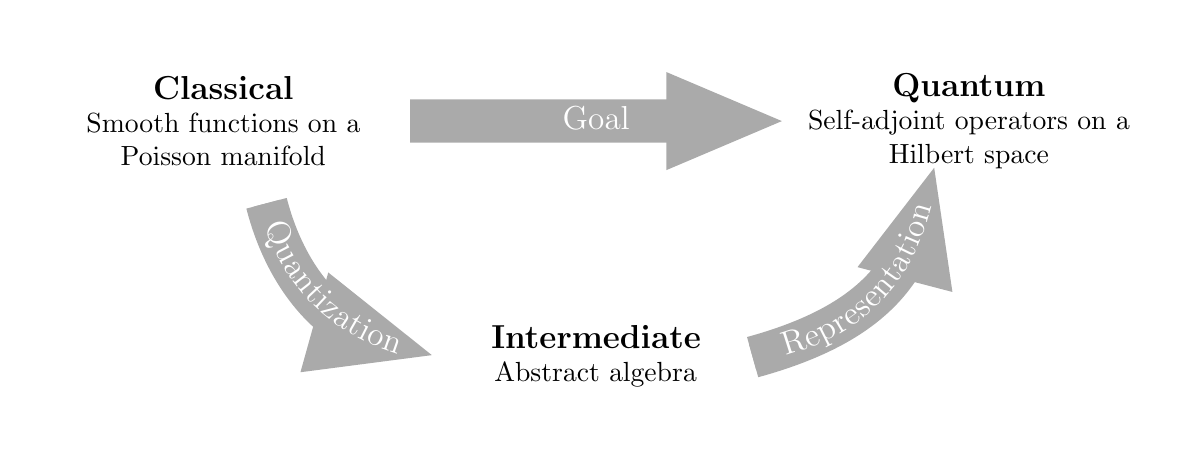
\begin{tikzpicture}
    	\tikzstyle{myarrowq} = 
    	[line width = 3.4mm,
    	draw = {rgb:black,1;white,2},
    	-triangle 45,
    	shorten >= -3mm,
    	postaction = {
    		draw, 
    		line width = 5.3mm, 
    		shorten >=4.5mm,
    		-},
    	postaction = {
    		decorate,
    		decoration = {
    			text along path, 
    			text = {|\large \color{white}| Quantization}, 
    			text align = {align = center},
    			raise = -0.7ex
    			}
    		},
    	]
    	\tikzstyle{myarrowg} = 
    	[line width = 3.2mm,
    	draw = {rgb:black,1;white,2},
    	-triangle 45,
    	postaction = {
    		draw, 
    		line width = 5.5mm, 
    		shorten >=6.5mm,
    		-},
    	postaction = {
    		decorate,
    		decoration = {
    			text along path, 
    			text = {|\large \color{white}| Goal }, 
    			text align = {align = center},
    			raise = -0.7ex
    			}
    		}
    	]
    	\tikzstyle{myarrowr} = 
    	[line width = 3.2mm,
    	draw = {rgb:black,1;white,2},
   		shorten >=-5mm,
   		shorten <=-4mm,
    	-triangle 45,
    	postaction = {
    		draw, 
    		line width = 5.3mm, 
    		shorten >=1.5mm,
    		-},
    	postaction = {
    		decorate,
    		decoration = {
    			text along path, 
    			text = {|\large \color{white}|Representations}, 
    			text align = {align = left},
    			raise = -0.6ex
    			}
    		}
    	]
    		    	
        \matrix (m)[
        matrix of nodes,
        row sep=3em,
        column sep=0pt,
		ampersand replacement=\&
        ]
        {
        	\parbox{4.5cm}
        	{
        	  \begin{center}
        		{\large
        			\textbf{Classical}
        		}
        		\\
        		{\normalsize
        			Smooth functions on
        			a Poisson manifold
        		}
        	  \end{center}
        	}
        	\&
        	\&
        	\parbox{4.5cm}
        	{
        	  \begin{center}
        		{\large
        			\textbf{Quantum}
        		}
        		\\
        		{\normalsize
        			Self-adjoint operators
        			on a Hilbert space
        		}
        	  \end{center}
        	}
        	\\
        	\&
        	\parbox{4.5cm}
        	{
        	  \begin{center}
        		{\large
        			\textbf{Intermediate}
        		}
        		\\
        		{\normalsize
        			Abstract algebra
        		}
        	  \end{center}
        	}
        	\&
        	\\
        };
        \draw
        [-stealth]
        (m-1-1) edge[myarrowg]					(m-1-3) 
        		edge[myarrowq, bend right=30]	(m-2-2)
        (m-2-2) edge[myarrowr, bend right=30]	(m-1-3)
		;
    \end{tikzpicture}
\end{center}


\subsubsection{Different approaches}
There exist various ideas about how to build up such a scheme. For example, in 
axiomatic quantum field theory one usually wants the quantum algebra to be a 
$C^*$-algebra (see for example \cite{haag:1993a} or 
\cite{baer.ginoux.pfaeffle:2007a}). The reason is that the bounded operators 
$\Bounded(\hilbert{H})$ naturally form such an algebra (and actually even more 
than that). Unfortunately, most of the operators in quantum mechanics are 
unbounded. This problem is cured by looking at the exponentiated operators
\begin{equation*}
	A
	\longmapsto
	\E^{i t A},
	\quad t \in \mathbb{R}.
\end{equation*}
This way, one gets a one parameter group for $t \in \mathbb{R}$ and unitary 
operators are clearly bounded. Moreover, there is a very nice correspondence 
between $C^*$-algebras and locally compact Hausdorff spaces, which is known as 
the Gelfand-Naimark theorem. Roughly stated, this means that there is an 
equivalence of categories between compact Hausdorff spaces and unital commutative 
$C^*$-algebras: every such space gives rise to a commutative algebra 
of complex-valued functions, which form a $C^*$-algebra. On the other hand, from 
every unital commutative $C^*$-algebra $\algebra{A}$ one can construct a 
compact Hausdorff space $X$ such that $\algebra{A} \cong \Stetig(X)$ . This 
correspondence can be extended to open and closed subsets of the space, to 
homeomorphism, locally compact spaces, their compactification, vector bundles and 
even more. There is a strong link between commutative algebra and topology or 
geometry. One possibility to think of a quantized system is to think of continuous 
or smooth functions on a noncommutative space, which then should correspond to a 
noncommutative $C^*$-algebra. This idea leads to noncommutative geometry, which 
is mostly due to Alain Connes. A very detailed, but not necessarily easy to read 
book is \cite{connes:1994a} by Connes, another and rather brief introduction is 
for example \cite{varilly:2006a}.


A different approach, called geometric quantization, tries to fulfil all 
of the three axioms (Q1) - (Q3) from the previous part. Unfortunately, this 
causes problems: already for a symplectic vector space, it is impossible to have a 
one-to-one correspondence of the Poisson bracket and the quantum mechanical 
commutator. This is known as the Groenewold-van Hove theorem, which was found 
around 1950 \cite{vanhove:1951a, groenewold:1946a}. More precisely spoken: no 
representation of the Lie algebra, which is generated by the $q^i$ and $p_j$ and 
which is defined by the classical commutation relations, can be extended 
irreducibly and faithfully to the commutator Lie algebra which comes from the 
associative unital algebra which is generated by the $q^i$ and $p_j$. Thus 
geometric quantization restricts to smaller observable algebras, which are not 
problematic. At its present state, this approach is however still far from being a 
general theory, but it provide a procedure for number of exemplary cases. Its 
ideas are mostly due to Souriau \cite{souriau:1970a}, Kostant and Segal.


There are also different approaches. Berezin proposed a quantization scheme for 
particular K\"ahler manifolds, \cite{berezin:1975a, berezin:1975b, berezin:1975c}. 
Still, new ideas keep coming up, but in the following, we want to concentrate on a 
particular type of quantization, which is called \emph{deformation quantization}.



\section{Deformation Quantization}
\label{sec:chap2_DQ}

\subsection{The Concept}
\label{subsec:chap2_Concept}

Deformation quantization tries to realize the three points (Q1) and (Q2) from the 
previous section, but weakens the third. If it is not possible to have such a 
correspondence exactly, we will at least want to have it 
\emph{asymptotically}. The motivating example is the Weyl quantization which we 
already talked about. There are actually two such formulas, that can be given: the 
first maps a function $f$ in the variables $q, p \in \mathbb{R}^n$ to a 
differential operator on $\mathbb{R}^n$, which is actually a formal power series 
in the parameter $\hbar$. For polynomial functions, this series is a sum (more 
precisely: a polynomial again) and well defined, for general functions this will 
really be a formal power series, hence a truly infinite sequence, which a priori 
has no analytical, but just an algebraic meaning. 
The second is given by an integral formula and holds for another class of 
functions (Schwartz functions), but one gets the first formula out of the second 
as an asymptotic expansion for $\hbar \longrightarrow 0$. With these 
quantizations, one can also define a product of two functions $f, g$, which will 
necessarily take those two functions to a formal power series in $\hbar$. Moyal 
showed that the commutator of this product can be understood as a series which 
approximates the quantum mechanical commutator \cite{moyal:1949a}. The reason why 
seemingly all of a sudden power series appear is the following: if one wants the 
correspondence principle to be asymptotically fulfilled, i.e.
\begin{equation*}
	[\mathcal{Q}(f), \mathcal{g}]
	=
	i \hbar \mathcal{Q}(\{ f, g \})
	+ \mathcal{O}(\hbar^2)
\end{equation*}
and the multiplication of these quantized functions to be associative 
(as needed for representations on the Hilbert space), one will necessarily get 
higher and higher orders in $\hbar$. This iteration can never be stopped without 
loosing associativity. Motivated by this observation, a group of mathematicians, 
the so called Dijon-school, started working out this idea of products as formal 
power series. They understood quantization as a \emph{deformation} of the 
commutative product by a formal parameter (mostly called $\hbar$, $\lambda$ or 
$\nu$, in this work we will call it $z$ from now on), which controls the 
noncommutativity of the theory. These deformed products should moreover fulfil 
some compatibility conditions with the classical theory. This was the 
hour of birth of deformation quantization. The main characters of this group 
were Flato, Lichnerowicz, Bayen, Fr{\o}nsdal and Sternheimer, who published 
their ideas in the late 70's \cite{bayen.et.al:1977a, bayen.et.al:1978a} and 
gave a first definition of a star product. These two articles became the starting 
point for what has now become a rich and fruitful theory. The deformed products 
are tits corner stone and one defines them in the following way.
\begin{definition}[Star Product]
	\label{Def:StarProduct}
	Let $(M, \{\cdot, \cdot\})$ be a Poisson manifold over a field 
	$\mathbb{K}$ ($\mathbb{K} = \mathbb{R}$ or $\mathbb{C}$).
	A star product on $M$ is a bilinear map
	\begin{equation*}
	    \star_z \colon 
    	\Cinfty(M) 
    	\times 
	    \Cinfty(M) 
	    \longrightarrow
	    \Cinfty(M) \llbracket z \rrbracket
	    , \
	    (f,g) 
	    \longmapsto 
	    f \star_z g 
	    =
	    \sum\limits_{n = 0}^\infty 
	    z^n C_n(f,g)
	\end{equation*}
	such that its $\mathbb{K}\llbracket z \rrbracket$-linear extension to 
	$\Cinfty(M) \llbracket z \rrbracket$ fulfils the following properties:
	\begin{definitionlist}
		\item
		$\star_z$ is associative.
		
		\item
		$C_0(f, g) = f \cdot g,\ \forall_{f,g \in \Cinfty(M)}$ (Classical limit).
		
		\item
		$C_1(f, g) - C_1(g, f)= z \{f, g\},\ \forall_{f,g \in \Cinfty(M)}$
		(Semi-classical limit).
		
		\item
		$1 \star_z f = f \star_z 1 = f,\ \forall_{f \in \Cinfty(M)}$.
	\end{definitionlist}
	If the $C_n$ are bidifferential operators, the star product is said to be 
	differential and if the order of differentiation of the $C_n$ does not 
	exceed $n$ in both arguments, a differential star product is said to be 
	natural. Moreover, we will say that a star product $\star_z$ is of Weyl-type,
	if $\cc{f \star_z g} = \cc{g} \star_z \cc{f}$ for all $f,g \in \Cinfty(M)$
	where $\cc{\phantom{a}}$ denotes the complex conjugation.
\end{definition}
They also defined a notion of equivalence of star products. The idea behind is 
that two equivalent star products should give rise to the same physics.
\begin{definition}[Equivalence of Star Products]
	Two star products $\star_z$ and $\widehat{\star}_z$ for a Poisson manifold 
	$(M, \{\cdot, \cdot\})$ are said to be equivalent, if there is a formal 
	power series
	\begin{equation*}
		T
		=
		\id +
		\sum\limits_{n=0}^{\infty}
		z^n T_n
	\end{equation*}
	of linear maps $T_n \colon \Cinfty(M) \longrightarrow \Cinfty(M)$, which 
	extends $\mathbb{K}\llbracket z \rrbracket$-linearly to 
	$\Cinfty(M) \llbracket z \rrbracket$, such that the following statements hold:
	\begin{equation*}
		f \star_z g
		=
		T^{-1}
		\left(
			T(f) \widehat{\star}_z T(g)
		\right)
		, \ 
		\forall_{f,g \in \Cinfty(M) \llbracket z \rrbracket}
		\quad \text{ and } \quad
		T(1) 
		= 
		1.
	\end{equation*}
	For differential or natural star products, we accordingly speak of 
	differential or 	natural equivalences.
\end{definition}
Note that these definitions are purely algebraic, since we do not ask for the
convergence of those power series. Hence the theory which was developed from 
this in the following years is also a mostly algebraic theory. Like for the Weyl 
product, there were also integral formulas around for other types of star products 
for which one can also make sense of convergence. But as already pointed out, one 
has to strongly restrict the algebra of functions, for example to the Schwartz 
space.



\subsection{A Mathematical Theory}
\label{subsec:chap2_MathTheory}
Deformation quantization is a good example for a mathematical theory, which is 
motivated by a physical idea. It is not really talking about a physical problem, 
since the world does not need to be quantized -- it already is. It is talking 
about a mathematical problem: how to recover the quantized (and very 
counter-intuitive) mathematics, which describe the world on very small scales out 
of the classical (and much more intuitive) mathematics, which describe the world 
on our scale? Deformation quantization tries to give an answer to that, but is 
unfortunately (at least at its present state) still far from doing so completely. 
Like many such theories, it started of from a more or less precise physical 
background and developed into something very different: a mostly algebraic, purely 
mathematical theory. That is also due to the fact that the questions, which had to 
be answered in the beginning, were very hard and of mathematical nature. It took a 
lot of time to find answers and meanwhile, the mathematicians working on them
were interested other aspects of the theory. We want to give a short overview of
those questions and their answers very briefly and summarize a bit the history of 
deformation quantization next. A more detailed summary can be found in section 6.1 
of \cite{waldmann:2007a}.


The prototype is, as already mentioned, a symplectic vector space, for which 
Weyl proposed a star product with a certain (symmetric) ordering (although the 
definition of a star product did not exist at his time). However, other 
orderings are possible: one can have a standard or an anti-standard ordering, 
where the $\hat p$'s are all ordered to the right or to the left, respectively, or 
something in  between. One of the first questions was, if one could also construct 
star products on symplectic manifolds and if these products will be standard or 
Weyl ordered, if they will be differential or natural and so on. Locally, the 
answer was yes, but it took some time and many small steps, until DeWilde and 
Lecomte could show that every cotangent bundle of a smooth manifold has star 
products \cite{dewilde.lecomte:1983a} and then extended this result to arbitrary 
smooth manifolds \cite{dewilde.lecomte:1983b}. Another proof was given 
independently from that by Omori, Maeda and Yoshioka 
\cite{omori.maeda.yoshioka:1991a} and then by Fedosov, who presented a simple 
and very geometric construction \cite{fedosov:1994a}, which always give rise to 
natural star products, as shown in \cite{bordemann.waldmann:1997a} 
or more generally in \cite{gutt.rawnsley:2003a}. Moreover, every star product on a 
symplectic manifold is equivalent to a Fedosov star product 
\cite{bertelson.cahen.gutt:1997a}. A lot of 
results were found for K\"ahler manifolds and also the already mentioned 
procedure, which is due to Berezin, gives rise to star products. There are 
moreover standard, anti-standard ordered and many other types of star products 
on every cotangent bundle. The next question was the one concerning the 
equivalence classes of star products in the symplectic case. One can show that 
locally, two star products on a symplectic manifold are always equivalent. Hence 
a classification result should depend on global phenomena. Indeed, this is the 
case and it can be shown that star products on a symplectic manifold are 
classified by its second deRham cohomology $\HdR^2(M)$. This result is due to 
Deligne \cite{deligne:1995a}, a different proof was given by Nest and Tsygan 
\cite{nest.tsygan:1995a}, another one by Bertelson, Cahen and Gutt 
\cite{bertelson.cahen.gutt:1997a}. More precisely: the choice of an equivalence 
class of closed, nondenerate 2-forms $\omega \in \Formen^2(M)$ determines a 
Fedosov star product and from every Fedosov 
star product one can calculate such an equivalence class. This already 
determines all star products on symplectic manifolds, since every star product 
on such a manifold is equivalent to a Fedosov star product. The case of Poisson 
manifolds took longer and was much harder to solve, since associativity turned 
out to be a complicated condition to fulfil. There were some examples of star 
products known for particular Poisson structure, like the Gutt star product 
\cite{gutt:1983a}, which was also found by Drinfel'd \cite{drinfeld:1983a} 
independently, but the general existence (and also the classification) result was 
proven by Kontsevich \cite{kontsevich:1997:pre, kontsevich:2003a} many years 
later. His classification result is known as the formality theorem and needs the 
notion of $L_{\infty}$-algebras, which are fairly involved objects. He gave an 
explicit construction, how star products can be built out of Poisson brackets on 
$\mathbb{R}^d$. This construction was extended by Cattaneo, Felder and Tomassini 
to Poisson manifolds \cite{cattaneo.felder.tomassini:2002b} and indepedently from 
that by Dolgushev \cite{dolgushev:2005a}. Another and easier formulation of the 
Kontsevich construction on $\mathbb{R}^d$ in terms of operads was later given by 
Tamarkin \cite{tamarkin:2003a}.



\subsection{From Formal to Strict}
\label{subsec:chap2_Formal2Strict}

So far, one could say that the big cornerstones of the theory are already there 
and that it is somehow ``finished''. For two reasons, this is not the case. 
First, a mathematical theory is never actually ``finished'', since there are 
always a lot of new things which can be found. There are still many different 
types of star products to classify, like invariant or equivariant star products 
in the case that one has Lie group or Lie algebra actions. A very recent result 
concerning the classification of equivariant star products on symplectic 
manifolds is, for example, due to Reichert and Waldmann 
\cite{reichert.waldmann:2015a:pre}. Second, the theory of deformation 
quantization still has a different aspect: all we talked about so far was purely 
algebraic and there is no notions of convergence of these formal power series. 
If some day, this theory shall have a real drawback on physics, it will be 
necessary to talk about the convergence properties of these star products, since 
in physics $\hbar$ is \emph{not} a formal parameter but a constant with a 
dimension and a fixed value and therefore the question of convergence matters. 
When we dace those problems and speak about continuous star products, we leave the 
field of \emph{formal} deformation quantization and come to \emph{strict} 
deformation quantization.


Although it is closer to physics, strict deformation quantization is still a 
mathematical theory. There are two different approaches to it: we 
already mentioned integral formulas, which allow to speak of continuous star 
products. The second approach uses the formal power series instead and wants to 
construct a topology on the polynomial algebra, such that the star product becomes 
continuous. Then one completes the tensor algebra over the vector space to a 
subalgebra of the smooth functions, on which the star product will still be 
continuous.


The first approach is mostly due to Rieffel, who developed these ideas in some of 
his papers \cite{rieffel:1989a, rieffel:1990c, rieffel:1993a}. He wants to 
realize a strict deformation quantization by actions of an abelian Lie group on a 
$C^*$-algebra of classical observables. Later Rieffel formulated a list of open 
questions, which strict deformation quantization should try to answer 
\cite{rieffel:1998a} in the next years. His approach was carried on by Bieliavsky 
and Gayral \cite{bieliavsky:2002a, bieliavsky.gayral:2015a}, who extended these 
concepts to much more general Lie groups and different manifolds. To get 
reasonably big observable algebras, they used oscillatory integrals and pushed 
this theory forward. A similar idea was realized by Natsume, Nest and 
Peter \cite{natsume.nest.peter:2003a}, who could show that under certain 
topological conditions, symplectic manifolds always admit strict deformations.


The second approach is due to Beiser and Waldmann 
\cite{beiser:2011a, beiser.waldmann:2014a, waldmann:2014a}. They restrict to the 
local situation, that means to Poisson structures on vector spaces. Then, they 
look at the polynomial functions on this vector spaces and try to find 
continuity estimates for them by constructing an explicit locally convex 
topology on the symmetric tensor algebra (which is isomorphic to the polynomial 
algebra). The aim is to make the topology as coarse as possible, to get then a 
large completion and hence a big quantized algebra of 
observables. There are two big advantages of this approach: the first one is 
that it can be applied to infinite dimensional vector spaces, what is necessary 
for quantum field theory, which deals with infinitely many degrees of freedom. 
The second is that we can really speak about all observables, also those 
which will correspond to unbounded operators, without having to exponentiate. In 
this sense, this idea is somehow more fundamental. The disadvantage is, however, 
that it is just a local theory at the moment. The idea is worked out just for 
one type of star products by now, which are star products of exponential type like 
the Weyl product. This means until now one can only control star products on 
symplectic vector spaces which come from a constant Poisson tensor 
\cite{waldmann:2014a}. This theory was carried on in the master thesis of Matthias 
Sch\"otz \cite{schoetz:2014a}, who rephrased it using semi-inner product, which 
are a somehow more physical notion, since one can interpret spaces with such a 
topology as projective limits of pre-Hilbert spaces. This also allows a slightly 
coarser topology and hence a larger completion of the symmetric tensor algebra.


In this work, we will follow the second approach and apply it to 
another type of star product, the Gutt star product, which comes from a linear 
Poisson tensor on a vector space. Of course, this is the next logical step after 
constant Poisson tensors. However, these are also the first \emph{non-symplectic}
Poisson structures, which will be strictly quantized this way. Thus this 
master thesis really contributes something new to the theory of strict 
deformation quantization: a second example, in which Waldmann's locally convex 
topology on the tensor algebra leads to a continuous star product, when 
considered as a power series and not as an integral. Note that this also has a 
certain effect on Lie theory: the result can be seen as a functorial 
construction for a locally convex topology on the universal enveloping algebra 
$\algebra{U}(\lie{g})$ of a (possibly infitely-dimensional) Lie algebra 
$\lie{g}$. Therefore they may have applications to, for example, the 
representation theory of $\algebra{U}(\lie{g})$.





% Chapter 3
%


%
% Chapter 3 of my master thesis:
% The first real chapter
%

\chapter{Algebraic Preliminaries}


\section{Linear Poisson structures in infinite dimensions}
\label{sec:chap3_LinearPoisson}

As we have seen before, there has already been done some work on how to 
strictly quantize Poisson structures on vector spaces. Star products of
exponential type on locally convex vector spaces were topologized by Stefan 
Waldmann in \cite{waldmann:2014a} and then investigated more closely by 
Matthias Schötz in \cite{schoetz:2014a}. Hence, as a the next step, we try
to attack linear Poisson structures on locally convex vector spaces. This 
will give a new big class of Poisson structures, which will be deformable in a 
strict way. Before we do so in the rest of this master thesis, we recall 
briefly some basics on linear Poisson structures.


We will always take a vector space $V$ and look at Poisson structures on the 
coordinates which are elements of the dual space $V^*$. In order to cover most 
of the physically interesting examples by our reflections, we will assume that 
$V$ is a locally convex vector space. Every finite-dimensional vector space is 
normable and complete and hence locally convex, so it fits in this framework. 
It is clear what $V^*$ should be and there is just one interesting topology on 
it. For infinite-dimensional spaces, the situation is more delicate:
we have to think about what coordinates should be and how a Poisson structure 
on them could look like. A priori, it is not clear which dual we should 
consider: the algebraic dual $V^*$ of all linear forms on $V$, or the 
topological dual $V'$ which contains just the continuous linear forms? Here, 
one could argue that only $V'$ is of real interest, since otherwise we would 
encounter the very strange effect of having discontinuous polynomials, and the 
aim of constructing a continuous star product on them seems somehow pointless. 
But even if we stick to $V'$, the question of the topology still remains: 
do we want to consider the weak or the strong topology there and why one of 
them should be more interesting. In any case, we have to choose a topology on 
this space. Once this is done, we have to think about a good notion of Poisson 
tensors in this context. However, we encounter quite a number of question,
which have no trivial answer. For this reason, it is worth looking at some 
equivalent formulations of $Pol(V^*)$ in the finite-dimensional case, since 
they may allow better generalizations.


Let $V$ be a finite dimensional vector space. Now, there is now question 
about the dual or its topology, since $V^* = V'$ is finite-dimensional, too, 
and we deal with polynomials on it. A linear Poisson structure on $V^*$ is 
something very familiar: it is equivalent to a Lie algebra structure on $V$.
\begin{proposition}
	\label{Alg:Prop:LinPoissonIsLieAlg}
	Let $V$ be a vector-space of dimension $n \in \mathbb{N}$ and $\pi \in 
	\Secinfty(\Anti^2(TV^*))$. Then the two following things are 
	equivalent:
	\begin{propositionlist}
		\item
		$\pi$ is a linear Poisson tensor.
		
		\item
		$V$ has a uniquely determined Lie algebra structure.
	\end{propositionlist}
\end{proposition}
\begin{proof}
	We choose a basis $e_1, \ldots, e_n \in V$ and denote its dual basis $e^1, 
	\ldots, e^n \in V^*$. Then we call the linear coordinates in these bases 
	$x_1, \ldots, x_n \in \Cinfty(V^*)$ and $\xi^1, \ldots, \xi^n \in 
	\Cinfty(V)$, such that for all $\xi \in V, x \in V^*$
	\begin{equation*}
		\xi
		=
		\xi^i(\xi) e_i
		\quad \text{ and } \quad
		x
		=
		x_i (x) e^i.
	\end{equation*}
	In these coordinates, the Poisson tensor reads
	\begin{equation*}
		\pi
		=
		\frac{1}{2}
		\pi_{ij}
		\frac{\partial}{\partial x_i}
		\wedge
		\frac{\partial}{\partial x_j},
	\end{equation*}
	where $\pi$ is linear in the coordinates and we have
	\begin{equation*}
		\pi_{ij}(x)
		=
		c_{ij}^k x_k.
	\end{equation*}
	This equivalent to a tensor
	\begin{equation*}
		c
		=
		\frac{1}{2}
		c_{ij}^k 
		e_k \tensor e^i \wedge e^j
	\end{equation*}
	which gives for $f,g \in \Cinfty(V^*)$
	\begin{equation}
		\label{Alg:KksInCoordinates}
		\{f, g\} (x)
		=
		\pi(df, dg)(x)
		=
		x_k c_{ij}^k 
		\frac{\partial f}{\partial x_i}
		\frac{\partial g}{\partial x_j},
	\end{equation}
	using the identification $T^*V^* \cong V^{**} \cong V$.
	But now, the statement is obvious, since antisymmetry of $\pi$ means
	antisymmetry of the $c_{ij}^k$ in the indices $i$ and $j$ and the Jacobi
	identity for the Poisson tensor gives
	\begin{equation}
		\label{Alg:JacobiInStructureConst}
		c_{ij}^\ell c_{\ell k}^m
		+
		c_{j k}^\ell c_{\ell i}^m
		+
		c_{ki}^\ell c_{\ell j}^m
		=
		0
	\end{equation}
	for all $i, j, k, m$, since it must be fulfilled for all smooth functions.
	Vicely versa, \eqref{Alg:JacobiInStructureConst} ensures the Jacobi 
	identity of $\pi$ in \eqref{Alg:KksInCoordinates}. Hence the map
	\begin{equation}
		\label{Alg:LieBracketOfKks}
		[ \cdot, \cdot ]
		\colon
		V
		\times
		V
		\longrightarrow
		V
		\quad
		(e_i, e_j)
		\longmapsto
		c_{ij}^k e_k
	\end{equation}
	defines a Lie bracket, since the $c_{ij}^k$ are antisymmetric and fulfil 
	the Jacobi identity and are therefore structures constants. Conversely, 
	the structure constants of a Lie algebra on $V$ define a Poisson tensor on 
	$V^*$ via \eqref{Alg:KksInCoordinates}.
\end{proof}


Since we know now, that $V$ is actually a Lie algebra, we will call it 
$\lie{g}$ from now on. Since they carry additional structure, these Poisson 
systems have a special name.
\begin{definition}[Kirillov-Kostant-Souriau bracket]
	\label{Def:KKS}
	Let $\lie{g}$ be a finite-dimensional Lie algebra. Then the Poisson 
	bracket $\{ \cdot , \cdot \}_{KKS}$, which is given by 
	Proposition~\ref{Alg:Prop:LinPoissonIsLieAlg} on $\lie{g}^*$ is called the 
	Kirillov-Kostant-Souriau bracket.
\end{definition}



The correspondence from Proposittion~\ref{Alg:Prop:LinPoissonIsLieAlg} is a 
first hint how we could extend our ideas to infinite dimensionsal systems. 
Unfortunately, we will not be able to find this nice 
correspondence of a Lie algebra structure on $\lie{g}$ and the linear 
polynomials on $\lie{g}'$, since the procedure we used involves the 
double-dual of $\lie{g}$. In general, this will be really bigger than 
$\lie{g}$ itself, and starting from some analogon of a linear Poisson 
structure on $\lie{g}'$, we will find a Lie algebra structure on $\lie{g}''$. 
Of course, we could just use the canonical embedding $\lie{g} \subseteq 
\lie{g}''$, but it could (and, in general, it will) happen, that the Lie 
bracket of $x,y \in \lie{g}$ will not be in $\lie{g}$ any more, but just in 
its double-dual. In most of the physical cases, we are actually not interested 
in the double-dual, but in the original vector space. Therefore, it seems to 
be a good choice to translate ''linear Poisson structure on $\lie{g}^*$'' as 
''$\lie{g}$ is a Lie algebra'' in infinite dimensions. Remark however that 
this is a choice and not a necessity, and other choices would have been 
possible.


The next task are the polynomials on $\lie{g}'$. As already mentioned, it is 
not easy to find a good generalization for them, since for a locally convex 
Lie algebra $\lie{g}$, even $\lie{g}'$ will be a rather huge vector space. 
Again, it is helpful to go back to the finite-dimensional case, where we have 
the following result:
\begin{proposition}
	\label{Alg:Prop:PolIsSym}
	Let $\lie{g}$ be a vector space of dimension $n \in \mathbb{N}$. Then 
	the algebras $\Sym^{\bullet}(\lie{g})$ and $\Pol^{\bullet}(\lie{g}^*)$ 
	are canonically isomorphic.
\end{proposition}
\begin{proof}
	since this is a very well-known result, we just want to sketch the proof 
	briefly: Take a basis $e_1, \ldots, e_n$ of $\lie{g}$ and its linear 
	coordinates $x_1, \ldots, x_n \in \Cinfty(\lie{g}^*)$ with $x_i(\xi) = 
	e_i(\xi)$ for $\xi \in \lie{g}^*$. On homogeneous symmetric tensors this 
	yields the map
	\begin{equation*}
		\mathcal{J}
		\colon
		\Sym^{\bullet}(\lie{g})
		\longrightarrow
		\Pol^{\bullet}(\lie{g}^*),
		\quad
		e_1^{\mu_1} \ldots e_n^{\mu_n}
		\longmapsto
		\xi_1^{\mu_1} \ldots \xi_n^{\mu_n}.
	\end{equation*}
	From the construction, we see that this is an isomorphism, but note, that 
	we have used the identification $\lie{g}^{**} \cong \lie{g}$ via
	\begin{equation*}
		e_i(\xi)
		=
		\langle \xi, e_i \rangle.
	\end{equation*}
\end{proof}
This gives a new idea for generalizing $\Pol(\lie{g}^*)$. One could argue that 
this isomorphism also uses the double dual which we wanted to avoid, since we 
could ''drop out'' of our original algebra and end up in $\Sym^{\bullet}
(\lie{g}^{**})$. Luckily, things are different now, and this is not possible. 
We can extend the Poisson bracket on $\lie{g}$ as a bi-derivation to 
$\Sym^{\bullet}(\lie{g})$ and get a closed Poisson algebra now. This way, we 
never even need to talk about $\Sym^{\bullet}(\lie{g}^{**})$. Of course, 
$\Sym^{\bullet}(\lie{g})$ only injects in $\Pol(\lie{g}')$ and we don't have 
an isomorphism any more, but we have good reason to think that this is enough: 
we get a closed and reasonably big subalgebra of of the polynomials. Moreover, 
the symmetric tensor algebra is defined on infinite-dimensional spaces 
exactly in the syme way as on finite-dimensional ones, there is no question 
about how to generalize, the construction is canonical.


Finally, we found a suitable way of speaking about object of interest: We 
replace linear Poisson structures on $\Pol^{\bullet}(\lie{g}^*)$ by 
$\Sym^{\bullet}(\lie{g})$. In finite dimension, this will not make a 
difference, but for the infinite-dimensional case, this is a choice and it is 
not mandatory to do it like this. Anyway, a decision had to be made and we 
have good reasons to believe that we are not completely misguided.



\section{The Gutt star product}
\label{sec:chap3_GuttStar}

Our final aim is to endow the symmetric algebra, and hence the polynomial 
algebra, with a new, noncommutative product. This is possible in a very 
natural way, due to the Poincar\'e-Birkhoff-Wit theorem. It links the 
symmetric tensor algebra $\Sym^{\bullet}(\lie{g})$ of a Lie algebra $\lie{g}$ 
to its universal enveloping algebra $\algebra{U}(\lie{g})$.


\subsection{The universal enveloping algebra}
\label{subsec:chap3_UniversalEnvelopingAlgebra}

If $\algebra{A}$ is an associative algebra, one can construct a Lie algebra 
out of it by using the commutator
\begin{equation*}
	[a,b]
	=
	a \cdot b - b \cdot a
	, \quad
	a,b \in \algebra{A}.
\end{equation*}
This construction is in fact functorial, since it doesn't only map associative 
algebras to Lie algebras, but also morphisms of the former to those of the 
latter. While getting a Lie algebra out of an associative algebra is easy, the 
reversed process is more complicated, but also possible. It is a well-known 
fact that every Lie algebra $\lie{g}$ can be embedded into an associative 
algebra, known as the universal enveloping algebra $\algebra{U}(\lie{g})$. It 
is uniquely determined (up to isomorphism) by the universal property: for 
every unital associative algebra $\algebra{A}$ and every homomorphism for Lie 
algebras $\phi\colon \lie{g} \longrightarrow \algebra{A}$ using the 
commutator on $\algebra{A}$, one gets a unital homomorphism of associative 
algebras $\Phi \colon \algebra{U}(\lie{g}) \longrightarrow \algebra{A}$ such 
that the following diagram is commutative:
\begin{center}
    \begin{tikzpicture}
        \matrix (m)[
        matrix of math nodes,
        row sep=2.5em,
        column sep=8em
        ]
        {
          \mathcal{U}(\lie{g}) & \\
           & \algebra{A} \\
          \lie{g} &  \\
        };
        \draw
        [-stealth]
        (m-1-1) 	edge node 
        			[above] 
        			{$\Phi$}
        					(m-2-2)
        	(m-3-1)	edge node
        			[below]
        			{$\phi$}
        					(m-2-2)
        					
        			edge node
        			[left]
        			{$\iota$}
        					(m-1-1)
        	;
    \end{tikzpicture}
\end{center}
The proof of existence and uniqueness of the universal enveloping algebra can 
be found in every standard textbook on Lie theory like 
\cite{hilgert.neeb:2012a} or \cite{varadarajan:1971a}, and we won't do it here 
in detail. Just recall that existence is proven by an explicit construction: 
one takes the tensor algebra $\Tensor^{\bullet}(\lie{g})$ and considers the 
two-sided ideal
\begin{equation*}
	\mathrm{I}
	=
	< \xi \tensor \eta - \eta \tensor \xi - [\xi, \eta] >
	, \quad
	\forall_{\xi, \eta \in \lie{g}}
\end{equation*}
inside of it. Then one gets the universal enveloping algebra by the quotient
\begin{equation}
	\label{Alg:UnivEnvAlg}
	\algebra{U}
	=
	\frac{\Tensor^{\bullet}(\lie{g})}{\mathrm{I}}.
\end{equation}
It follows from this construction, that $\algebra{U}(\lie{g})$ is a filtered 
algebra
\begin{equation*}
	\algebra{U}(\lie{g})
	=
	\bigcup_{k \in \mathbb{N}}
	\algebra{U}^k(\lie{g})
	, \quad
	\algebra{U}^k(\lie{g})
	= 
	\Big\lbrace
		x 
		= 
		\sum_i
		\xi_1^i \cdot \ldots \cdot \xi_n^i
	\ \Big| \ 
		\xi_j^i \in \lie{g}
		, \
		1 \leq j \leq n,
		i \in \mathbb{N}
	\Big\rbrace.
\end{equation*}
We just get a filtration, not a graded structure, however, since the ideal 
$\mathrm{I}$ is not homogeneous. Moreover, $\algebra{U}(\lie{g})$ is 
commutative (and graded) if and only if $\lie{g}$ was commutative. But 
$\algebra{U}(\lie{g})$ is much more than an associative algebra: it is also a 
Hopf algebra, since one can define a coassociative, cocommutative coproduct on 
it
\begin{equation*}
	\Delta \colon
	\algebra{U}(\lie{g})
	\longrightarrow
	\algebra{U}(\lie{g})
	\tensor
	\algebra{U}(\lie{g})
	, \quad
	\xi
	\longmapsto
	\xi \tensor \Unit
	+
	\Unit \tensor \xi
	, \quad
	\forall_{\xi \in \lie{g}}
\end{equation*} 
which extends to $\algebra{U}(\lie{g})$ via algebra homomorphism, as well as an antipode
\begin{equation*}
	S \colon
	\algebra{U}(\lie{g})
	\longrightarrow
	\algebra{U}(\lie{g})
	, \quad
	\xi
	\longmapsto
	- \xi
	, \quad
	\forall_{\xi \in \lie{g}}
\end{equation*}
which extends to $\algebra{U}(\lie{g})$ via algebra antihomomorphism.

\subsection{The Poincar\'e-Birkhoff-Witt theorem}
\label{subsec:chap3_PoincareBirkhoffWitt}

It is a well-known fact that one has a basis in $\algebra{U}(\lie{g})$. This 
result is due to the already mentioned theorem of Poincar\'e, Birkhoff and 
Witt:
\begin{theorem}[Poincar\'e-Birkhoff-Witt theorem]
	\label{Thm:Alg:PBW}
	Let $\lie{g}$ be a Lie algebra with a basis $\mathcal{B}_{\lie{g}} = \{ 
	\beta_i \}_{i \in I}$. Then the set
	\begin{equation*}
		\mathcal{B}_{\algebra{U}(\lie{g})}
		=
		\big\{
			\beta_{i_1}^{\mu_{i_1}}
			\cdot \ldots \cdot
			\beta_{i_n}^{\mu_{i_n}}
		\ \big| \
			n \in \mathbb{N}, \ 
			i_k \in I
			\text{ with } i_1 \earlier \ldots \earlier i_n 
			\text{ and } \beta_{i_k} \in \mathcal{B}_{\lie{g}}, \
			\mu_{i_1}, \ldots, \mu_{i_n} \in \mathbb{N}
		\big\}
	\end{equation*}
	defines a basis of $\algebra{U}(\lie{g})$.
\end{theorem}
there are different proofs for this statement. While a geometrical proof is 
very convenient in the finite-dimensional case, a combinatorial argument must 
be used in infinite dimensions. Most textbooks give the latter one, but 
restrict to finite-dimensional Lie algebras in order to avoid speaking of 
basis in infinite dimensions (except, of course, \cite{bourbaki:}). Once one 
has accepted working with the Lemma of Zorn, the proof will work the same way 
for any Lie algebra, since the idea relies on ordered index sets which can be 
defined in any dimension.
The PBW theorem allows us to set up an isomorphism between $\Sym^{\bullet}
(\lie{g})$ and $\algebra{U}(\lie{g})$ immediately, since a basis of the former 
can be given by almost the same expression
\begin{equation*}
	\mathcal{B}_{\Sym^{\bullet}(\lie{g})}
	=
	\big\{
		\beta_{i_1}^{\mu_{i_1}}
		\ldots
		\beta_{i_n}^{\mu_{i_n}}
	\ \big| \
		n \in \mathbb{N}, \ 
		i_k \in I, 1 \leq k \leq n,
		i_1 \earlier \ldots \earlier i_n 
		\text{ and } \beta_{i_k} \in \mathcal{B}_{\lie{g}}, \
		\mu_{i_1}, \ldots, \mu_{i_n} \in \mathbb{N}
	\big\}
\end{equation*}
where we just have replaced the noncommutative product in $\algebra{U}
(\lie{g})$ by the symmetric tensor product $\vee$ (which we will usually 
denote without a symbol, if possible) in $\Sym^{\bullet}(\lie{g})$. This 
allows us to write down an isomorphsim between the symmetric tensor algebra 
and the universal enveloping algebra, just by mapping the basis vectors to 
each other in a naive way. Of course, this can never be an isomorphism in the 
sense of algebras, but only of (filtered) vector spaces, because one of the 
algebras is commutative and the other isn't. Moreover, the symmetric algebra 
has a grading in the sense that
\begin{equation*}
	\Sym^{\bullet}(\lie{g})
	=
	\bigoplus\limits_{n = 0}^{\infty}
	\Sym^n(\lie{g})
	, \quad
	\Sym^n(\lie{g})
	=
	\underbrace{
		\lie{g} \vee \ldots \vee \lie{g}
	}_{
		n \text{ times}
	},
\end{equation*}
which induces a filtration by $\Sym^{(k)}(\lie{g}) = \sum_{j=0}^k 
\Sym^j(\lie{g})$. Our simple isomorphism will respect the filtration, but it 
isn't the only isomorphism which one can write down. In \cite{berezin:1971a}, 
Berezin proposed another isomorphism which is more helpful to use:
\begin{equation}
	\label{Alg:BerezinQuantization}
	\mathfrak{q}_n
	\colon
	\Sym^n(\lie{g})
	\longrightarrow
	\algebra{U}^n(\lie{g})
	, \quad
	\beta_{i_1} \ldots \beta_{i_n}
	\longmapsto
	\frac{1}{n!}
	\sum\limits_{\sigma \in S_n}
	\beta_{i_{\sigma(1)}} 
	\cdot \ldots \cdot
	\beta_{i_{\sigma(n)}}
	, \quad
	\mathfrak{q}
	=
	\sum\limits_{n = 0}^{\infty}
	\mathfrak{q}_n.
\end{equation}
We will refer to it as the quantization map, for reasons that will soon become 
clear. It also respects the filtration and transfers the symmetric product to 
another symmetric expression. In this sense, we can now switch between both 
algebras and use the setting, which is more convenient in the current 
situation: the graded structure of $\Sym^{\bullet}(\lie{g})$, or the Hopf 
algebra structure of $\algebra{U}(\lie{g})$.


\subsection{The Gutt star product}
Since we know, that the universal enveloping and the symmetric tensor algebra 
are isomorphic as vector spaces, we have a good tool at hand to endow the 
symmetric tensor algebra, and hence the polynomials, with a noncommutative 
product. This is exactly what Gutt did in \cite{gutt:1983a}. She constructed a 
star product on $\Pol^{\bullet}(\lie{g}^*)$ by pulling back the one from 
$\algebra{U}(\lie{g})$ while encoding the noncommutativity in a formal 
parameter $z \in \mathbb{C}$ in a convenient way. 
\begin{definition}[Gutt star product]
	\label{Def:GuttStar}
	Let $\lie{g}$ be a Lie algebra, $z \in \mathbb{C}$, and 
	$f, g \in \Sym^{\bullet}(\lie{g})$ of degree $k$ and $\ell$ respectively. 
	Then we define the Gutt star product:
	\begin{equation}
		\star_z
		\colon
		\Sym^{\bullet}(\lie{g})
		\times
		\Sym^{\bullet}(\lie{g})
		\longrightarrow
		\Sym^{\bullet}(\lie{g})
		, \quad
		(f,g)
		\longmapsto
		\sum\limits_{n = 0}^{e + \ell - 1}
		z^n
		\pi_{k + \ell - n}
		\left(
			\mathfrak{q}^{-1} \left(
				\mathfrak{q}(f) \cdot \mathfrak{q}(g)
			\right)
		\right),
	\end{equation}
	where the $\pi_n \colon \Sym^{\bullet}(\lie{g}) \longrightarrow 
	\Sym^n(\lie{g})$ are the projections on the homogeneous components of 
	degree $n$. 
\end{definition}
This is the original way in which Gutt defined her star product in 
\cite{gutt:1983a}, but there are two more ways to do it. Define
\begin{equation*}
	\mathrm{I}_z
	=
	< \xi \tensor \eta - \eta \tensor \xi - z [\xi, \eta] >
\end{equation*}
for $z \in \mathbb{C}$. Then we set 
\begin{equation}
	\label{Alg:DeformedUnivEnvAlg}
	\algebra{U}(\lie{g}_z)
	=
	\frac{\Tensor^{\bullet}(\lie{g})}{\mathrm{I}_z},
\end{equation}
and get the map
\begin{equation}
	\label{Alg:DeformedQuantization}
	\mathfrak{q}_{z,n}
	\colon
	\Sym^n(\lie{g})
	\longrightarrow
	\algebra{U}^n(\lie{g}_z)
	, \quad
	\beta_{i_1} \ldots \beta_{i_n}
	\longmapsto
	\frac{1}{n!}
	\sum\limits_{\sigma \in S_n}
	\beta_{i_{\sigma(1)}} 
	\cdot \ldots \cdot
	\beta_{i_{\sigma(n)}}
	, \quad
	\mathfrak{q}_z
	=
	\sum\limits_{n = 0}^{\infty}
	\mathfrak{q}_{z, n}.
\end{equation}
This way, we also get a star product:
\begin{equation}
	\label{Alg:DeformedStar}
	\widehat{\star}_z
	\colon
	\Sym^{\bullet}(\lie{g})
	\times
	\Sym^{\bullet}(\lie{g})
	\longrightarrow
	\Sym^{\bullet}(\lie{g})
	, \quad
	(f,g)
	\longmapsto
	\mathfrak{q}_z^{-1} 
	\left(
		\mathfrak{q}_z(f) \cdot \mathfrak{q}_z(g)
	\right).
\end{equation}
In \cite{drinfeld:1981a}, Drinfeld also constructed a star product using the 
Baker-Campbell-Hausdorff series: take $\xi, \eta \in \lie{g}$ and set
\begin{equation}
	\label{Alg:DrinfeldStar}
	\exp(\xi) \ast_z \exp(\eta)
	=
	\exp \left(
		\frac{1}{z}
		\bch{z \xi}{z \eta}
	\right),
\end{equation}
where the exponential series is understood a formal power series in $\xi$ and 
$\eta$. By differentiating, on gets the star product on all polynomials.


Of course, our aim is to show that these three maps are in fact identical and 
that they define a star product. Since this is a long way to go, we postpone 
the proof to the end of this chapter. It will be useful to learn something 
about the Baker-Campbell-Hausdorff series and the Bernoulli number first.



\section{The Baker-Campbell-Hausdorff series}
\label{sec:chap3_BCH}

Since we have a formula for $\star_z$ which involves the
Baker-Campbell-Hausdorff series, we want to give a short overview
about it and introduce some results, that will be helpful later on.
Note however, that there is not \emph{the} BCH formula, since one can always 
rearrange terms using antisymmetry, Jacobi and higher identities, but for 
$\xi, \eta \in \lie{g}$ for some Lie algebra $\lie{g}$, we can always write it 
as
\begin{equation}
	\label{Alg:NamesOfBCH}
	\bch{\xi}{\eta}
	=
	\sum\limits_{n = 1}^{\infty}
	\bchpart{n}{\xi}{\eta}
	=
	\sum\limits_{a,b = 0}^{\infty}
	\bchparts{a}{b}{\xi}{\eta},
\end{equation}
where $\bchpart{n}{\xi}{\eta}$ denotes all expressions having $n$ letters and 
$\bchparts{a}{b}{\xi}{\eta}$ denotes all expressions with $a$ $\xi$'s and $b$ 
$\eta$'s. Clearly we have
\begin{equation*}
	\bchpart{n}{\xi}{\eta}
	=
	\sum\limits_{b + b = n}
	\bchparts{a}{b}{\xi}{\eta}.
\end{equation*}
This only postpones the problem of non-uniqueness to the partial expressions, 
but it will be helpful, since we don't have to choose a special form for 
writing BCH every time.



\subsection{Some general and historical remarks}
Let a noncommutative algebra $\algebra{A}$ be given. For $\xi, \eta \in 
\algebra{A}$ we look at the identity
\begin{equation*}
	\exp(\chi)
	=
	\exp(\xi)
	\exp(\eta).
\end{equation*}
Then, algebraically speaking, the BCH series is the formal power series for 
$\chi$ as a commutator expression in $\xi$ and $\eta$. We can take the formal 
power series for the exponentials
\begin{equation*}
	\exp(\xi)\exp(\eta) 
	= 
	\sum\limits_{n,m=0}^{\infty} 
	\frac{\xi^n \eta^m}{n! m!}
\end{equation*}
and use the formal power series for the logarithm
\begin{equation*}
	\log(\chi) 
	= 
	\sum\limits_{k = 1}^{\infty} 
	\frac{ (-1)^{k-1} }{ k } (\chi - 1)^k.
\end{equation*}
This yields
\begin{equation}
	\label{Alg:BCHinRaw}
	\chi
	= 
	\log \left( \exp(\xi) \exp(\eta) \right) 
	= 
	\sum\limits_{k = 1}^{\infty} 
	\frac{ (-1)^{k - 1} }{k} 
	\sum\limits_{ \substack{ 
		i \in \{1, \ldots, k\} \\ 
		n_i, m_i \geq 0 \\ n_i + m_i \geq 1
	}}
	\frac{
		\xi^{n_1} \eta^{m_1} 
		\ldots 
		\xi^{n_k} \eta^{m_k}
	}
	{n_1! m_1! \ldots n_k! m_k!}.
\end{equation}
It is obviously far from trivial, if and how this can be expressed using 
commutators, and the first one to find a general way for this was Dynkin in 
the 1950's.


Now let $\lie{g}$ be a finite-dimensional Lie algebra with a corresponding Lie 
group $G$. From the geometric point of view, the BCH formula is the 
infinitesimal counterpart of the multiplication law in $G$. One can express it 
as a series of Lie brackets, which converges just in a small neighbourhood 
around the unit element $e \in G$. Since the exponential function  $\exp 
\colon \lie{g} \longrightarrow G$ is locally diffeomorphic there, one gets for 
$\xi, \eta \in \lie{g}$
\begin{align*}
	\bch{\xi}{\eta}
	& =
	\log \left( \exp(X) \exp(Y) \right)
	\\
	& =
	\xi + \eta
	+ \frac{1}{2} [\xi, \eta]
	+ \frac{1}{12} ( [\xi, [\xi, \eta]] + [\eta, [\eta, \xi]] )
	+ \ldots
\end{align*}
The formula was recovered by Campbell \cite{campb1, campb2}, Baker 
\cite{baker} and Hausdorff \cite{hausd} independently, founding on a work by 
Schur \cite{schur}. A lot of work has been done on it since, and one can find 
a nice summary about it in the introductory part of \cite{casmur}.


\subsection{Forms of the BCH}
As already mentioned, there are different forms of stating the BCH formula and 
depending on the problem one wants to solve, not each one is well suited. One 
can classify them roughly into four groups.
\begin{enumerate}
	\item
	There are recursive formulas, which calculate each term from the previous 
	one. The first expression due to Baker, Campbell and Hausdorff were of 
	this kind. Though the idea is old, this approach is still much used and 
	allows powerful applications: Casas and Murua found an efficient 
	algorithms \cite{casas.murua:yeara} for calculating the BCH series up to 
	high orders, based on a recursive formula given by Varadarajan in his 
	textbook \cite{varadarajan:yeara}.
	
	\item
	Most textbooks prove an integral form of the series, like 
	\cite{hall:yeara} and \cite{hilgert.neeb:2012a}. since we will use it, 
	too, we want to introduce it here briefly. Take the meromorphic function
	\begin{equation}
		\label{Alg:DefinitionLogBernoullis}
		g \colon 
		\mathbb{C}
		\longrightarrow
		\mathbb{C},
		\quad
		z 
		\longmapsto
		\frac{ z \log(z) }{z - 1}
	\end{equation}
	and denote for $\xi \in \lie{g}$ by
	\begin{equation*}
		\ad_{\xi}
		\colon
		\lie{g}
		\longrightarrow
		\lie{g},
		\quad
		\eta
		\longmapsto
		[\xi, \eta]
	\end{equation*}
	the usual ad-operator. Then one has for $\xi, \eta \in \lie{g}$
	\begin{equation}
		\label{Alg:BCHinIntegral}
		\bch{\xi}{\eta}
		=
		\xi + 
		\int\limits_0^1
		g \left( 
			\exp \left(
				\ad_{\xi}
			\right)
			\exp \left(
				t \ad_{\eta}
			\right)
		\right)
		(\eta) 
		dt.
	\end{equation}
	
	\item
	As already mentioned, Dynkin found a closed form for \eqref{Alg:BCHinRaw},
	which is the only one of this kind known so far. One can its proof for 
	example in \cite{jacobson:yeara}. It reads
	\begin{equation}
		\label{Alg:BCHinDynkin}
		\bch{\xi}{\eta}
		=
		\sum\limits_{k = 1}^{\infty} 
		\frac{ (-1)^{k - 1} }{k}
		\sum\limits_{\substack{
			i \in \{1, \ldots, k\} \\
			n_i, m_i \geq 0 \\ 
			n_i + m_i \geq 1
		}}
		\frac{1}{ \sum_{i = 1}^k(n_i + m_i) }
		\frac{ \left[
			\xi^{n_1} \eta^{m_1} \ldots \xi^{n_k} \eta^{m_k}
		\right]}
		{ n_1! m_1! \ldots n_k! m_k! },
	\end{equation}
	where the expression $[ \ldots ]$ denotes Lie brackets nested to the left:
	\begin{equation*}
		[\xi \eta \eta \xi]
		=.
		[[[\xi, \eta], \eta], \xi]
	\end{equation*}
	Unfortunately, the combinatorics get extremely complicated for higher 
	degrees, since it contains a lot of redundancies.
	
	\item
	Goldberg gave a form of the series which is based on words in two letters:
	\begin{equation}
		\bch{\xi}{\eta}
		=
		\sum\limits_{n = 1}^{\infty}
		\sum\limits_{|w| = n}
		g_w w.
	\end{equation}
	The $g_w$ are coefficients, which can be calculated using the recursively
	defined Goldberg polynomials (see \cite{goldberg:1956a}). It was put into 
	commutator form by Thompson in \cite{thompson:1982a}:
	\begin{equation}
		\label{Alg:BCHinGoldbergThompson}
		\bch{\xi}{\eta}
		=
		\sum\limits_{n = 1}^{\infty}
		\sum\limits_{|w| = n}
		\frac{g_w}{n} [w].
	\end{equation}
	Again, the $[w]$ are Lie brackets nested to the left. Of course, this 
	formula will also have redundancies, but its combinatorial aspect is much 
	easier than the one of \eqref{Alg:BCHinDynkin}. Since there are estimates 
	for the coefficients $g_w$, we will use this form for our Main Theorem.
\end{enumerate}


\subsection{The Goldberg-Thompson formula and some results}

\subsubsection{Goldberg's theorems}
We now introduce the results of Goldberg: he noted a word in the letters $\xi$ 
and $\eta$ as
\begin{equation*}
	w_{\xi}(s_1, s_2, \ldots, s_m)
	=
	\xi^{s_1} \eta^{s_2} \ldots (\xi \vee \eta)^{s_m},
\end{equation*}
with $m \in \mathbb{N}$ and the last letter will be $\xi$ if $m$ is odd and 
$\eta$ if $m$ is even. The index $\xi$ of $w_{\xi}$ means, that the word 
starts with a $\xi$. Now we can assign to each word $w_{\xi \vee \eta}(s_1, 
\ldots, s_m)$ a coefficient $c_{\xi \vee \eta}(s_1, \ldots, s_m)$. This is 
done by the following formula:
\begin{equation}
	\label{Alg:GoldbergCoeff1}
	c_{\xi}(s_1, \ldots, s_m) 
	= 
	\int\limits_0^1 
	t^{m'} (t - 1)^{m''} 
	G_{s_1}(t) \ldots G_{s_m}(t) dt,
\end{equation}
where we have $m' = \lfloor \frac{m}{2} \rfloor$, $m'' = \lfloor \frac{m-1}{2} 
\rfloor$ with $\lfloor \cdot \rfloor$ denoting the entire part of a real 
number and we have $n = \sum_{i = 1}^m s_i$. For $c_{\eta}$ we have
\begin{equation}
	\label{Alg:GoldbergCoeff2}
	c_{\eta}\left( s_1, \ldots, s_m \right)
	= 
	\begin{cases}
		c_{\xi}\left( s_1, \ldots, s_m \right)
		& 
		\text{ if } m \text{ is odd} 
		\\
		(-1)^{n-1} c_{\xi} \left( s_1, \ldots, s_m \right)
		& 
		\text{ if } m \text{ is even.}
	\end{cases}
\end{equation}
The $G_s$ are the recursively defined Goldberg polynomials
\begin{equation}
	\label{Alg:GoldbergPolynomials}
	G_s(t) 
	= 
	\frac{1}{s} 
	\frac{d}{dt} 
	t(t-1) G_{s-1}(t),
\end{equation}
for $s > 1$ and $G_1(t) = 1$. From \eqref{Alg:GoldbergCoeff2} we get 
immediately
\begin{equation*}
	c_{\xi}\left( s_1, \ldots, s_m \right)
	= 
	c_{\eta}\left( s_1, \ldots, s_m \right) 
	= 
	0 
	\quad 
	\text{ if $m$ is odd and $n$ is even.}
\end{equation*}
Of course, Goldberg found interesting identities which are fulfilled by the 
coefficients. A very remarkable one is that for all permutations $\sigma \in 
S_m$ one has
\begin{equation*}
	c_{\xi}\left( s_1, \ldots, s_m \right)
	=
	c_{\xi}\left( s_{\sigma(1)}, \ldots, s_{\sigma(m)} \right),
\end{equation*}
since \eqref{Alg:GoldbergCoeff1} obviously doesn't see the ordering of the 
$s_i$ and $m'$, $m''$ and $n$ are not affected by reordering. For words with 
$m = 2$, an easier formula can be found:
\begin{equation*}
	c_{\xi}(s_1, s_2) 
	= 
	\frac{ (-1)^{s_1} }{s_1! s_2!} 
	\sum\limits_{n = 1}^{s_2} 
	\binom{s_2}{n} B_{s_1 + s_2 - n},
\end{equation*}
where the $B_s$ denote the Bernoulli numbers, which will be explained more 
precisely in the next paragraph. First, we note that the only case which 
matters to us is of course $s_1 = 1$, since for $s_1, s_2 > 1$ we will find 
something like $[[\xi, \xi], \ldots ] = 0$. For simplicity, let's set 
$s_2 = 1$ and to permute $s_1 \leftrightarrow s_2$:
\begin{equation}
	\label{Alg:GoldbergCoeffBernoulli}
	c_{\xi}(1, n-1)
	=
	\frac{ (-1)^{n-1} }{s!}
	B_s.
\end{equation}


\subsubsection{Bernoulli numbers}
We have seen the Bernoulli numbers $B_n$ showing up and we will encounter them 
very often in the following. Hence it is useful to learn a few important 
things about them. They are defined by the series expansion of
\begin{equation}
	\label{Alg:DefBernoulli}
	g \colon
	\mathbb{C}
	\longrightarrow
	\mathbb{C}
	, \quad
	z \longmapsto
	\frac{z}{\E^z - 1}
	=
	\sum\limits_{n=0}^{\infty}
	\frac{B_n}{n!}z^n.
\end{equation}
Clearly, $g$ has poles at $z = 2 k \pi i$, $k \in \mathbb{Z}\backslash \{0\}$.
Moreover, one can easily show that all odd Bernoulli numbers are zero, except 
for $B_1 = - \frac{1}{2}$ and since in some applications one needs $B_1$ to be 
positive, there is a different convention for naming them: one often 
encounters $B_n^* = (-1)^n B_n$ (which only differs for $n = 1$). The nonzero 
Bernoulli number alternate in sign and for there absolute value, one can show 
the asymptotic behaviour (see \cite{luschny.oeis})
\begin{equation*}
	B_{2n} 
	\sim 
	(-1)^{n-1} 
	4\sqrt{\pi n} 
	\left( \frac{n}{\pi e} \right)^{2n}.
\end{equation*}
This is not surprising, since we now that the generating function $g$ had 
poles at $\pm 2\pi i$. The Bernoulli numbers can also be calculated by the 
recursion formula
\begin{equation}
	B_n
	=
	- \frac{1}{n + 1}
	\sum\limits_{k = 0}^{n- 1}
	\binom{n + 1}{k}
	B_k,
\end{equation}
which is well-known in the literature. Since we will deal a lot with them, we 
want to give the first numbers of this series here.
\begin{center}
	\begin{tabular}
	{c||c|c|c|c|c|c|c|c|c|c|c|c|c|c|c|c|c}
		$n$ & $0$ & $1$ & 
		$2$ & $3$ & $4$ & 
		$5$ & $6$ & $7$ & 
		$8$ & $9$ & $10$ & 
		$11$ & $12$ & $13$ & 
		$14$ & $15$ & $16$
		\\
		\hline 
		$B_n$ & $1$ & $-\frac{1}{2}$ & 
		$\frac{1}{6}$ & $0$ & $-\frac{1}{30}$ & 
		$0$ & $\frac{1}{42}$ & $0$ & 
		$-\frac{1}{30}$ & $0$ & $\frac{5}{66}$ & 
		$0$ & $\frac{691}{2730}$ & $0$ & 
		$\frac{7}{6}$ & $0$ & $\frac{3617}{510}$
	\end{tabular} 
\end{center}


\subsubsection{BCH up to first order}

\begin{proposition}
	Let $\lie{g}$ be a Lie algebra and the Bernoulli numbers as defined 
	before. Then we have for $\xi, \eta \in \lie{g}$
	\begin{align}
		\label{Alg:BCHFirstOrderXi}
		\bch{\xi}{\eta}
		& =
		\sum\limits_{n = 0}^{\infty}
		\frac{B_n^*}{n!}
		\left( \ad_{\xi} \right)^n (\eta)
		+ \mathcal{O} \left( \eta^2 \right)
		\\
		\label{Alg:BCHFirstOrderEta}
		& =
		\sum\limits_{n = 0}^{\infty}
		\frac{B_n}{n!}
		\left( \ad_{\xi} \right)^n (\eta)
		+ \mathcal{O} \left( \xi^2 \right)
	\end{align}
\end{proposition}
\begin{proof}
	This is something we can perfectly calculate using the Goldberg 
	coefficients. Remind that we will put words to Lie brackets, and for 
	computing the coefficients we will need the words $\eta \xi^n$ \emph{and} 
	$\xi \eta \xi^{n-1}$ because of antisymmetry. Now let $n \in \mathbb{N}$. 
	We have
	\begin{equation*}
		c{\eta}(1,n) 
		= 
		(-1)^n c_{\xi}(1,n) 
		= 
		(-1)^n 
		\frac{(-1)^n}{n!} 
		B_n 
		= 
		\frac{B_n}{n!}.
	\end{equation*}
	By $n-fold$ skew-symmetry and \eqref{Alg:BCHinGoldbergThompson}, we get 
	the contribution
	\begin{equation*}
		\frac{(-1)^n}{(n+1)!} 
		B_n \left( \ad_{\xi} \right)^n (\eta)
		=
		\frac{1}{(n+1)!} 
		B_n^* \left( \ad_{\xi} \right)^n (\eta)		
	\end{equation*}
	Now we need $c_{\xi}(1, 1, n-1)$: let $n > 1$, then
	\begin{align*}
		c_{\xi}(1, 1, n - 1) 
		& = 
		\int\limits_0^1 
		t(t-1) G_{n-1}(t) 
		dt 
		\\
		& = 
		- \int\limits_0^1 
		t \frac{d}{dt} 
		\left( t(t-1) G_{n-1}(t) \right) 
		dt 
		\\
		& =
		- \int\limits_0^1 
		n t G_n(t) 
		dt 
		\\
		& = 
		-n 
		c_{\xi}(1,n) 
		\\
		& = 
		-n 
		\frac{(-1)^n}{n!} 
		B_n 
		\\
		& =  
		(-1)^{n + 1} 
		\frac{1}{(n-1)!} B_n
	\end{align*}
	So by using $n-1$ times the skew-symmetry of the Lie bracket, we get
	\begin{equation*}
		\frac{1}{n + 1} 
		\cdot (-1)^{n + 1} 
		\frac{1}{ (n - 1)! }
		B_n 
		[\ldots [\xi, \eta], \xi] \ldots ], \xi] 
		= 
		\frac{n}{(n+1)!} 
		B_n 
		\left( \ad_{\xi} \right)^n (\eta)
	\end{equation*}
	For $n > 1$, we add up those two and use the fact that $B_n = B_n^*$ and 
	find the result we want. For $n = 1$, there is just the first contribution 
	and $c_{\xi}(1,1) = - B_1$, which gives
	\begin{equation*}
		B_1^* \ad_{\xi}(\eta)
	\end{equation*}
	in total. For $n = 0$ , we get $c_{\xi}(1) = c_{\eta}(1) = 1$ and finally 
	get \eqref{Alg:BCHFirstOrderXi}. For \eqref{Alg:BCHFirstOrderEta}, note 
	that we need $c_{\xi}(1, n)$ and $c_{\eta}(1, 1, n-1)$. We have 
	$c_{\xi}(1,n) = (-1)^n c_{\eta}(1,n)$ and 
	$c_{\eta}(1, 1, n-1) = (-1)^n c_{\xi}(1,1,n-1$.
	this gives a global $(-1)^n$ and makes hence $B_n$ out of $B_n^*$.
\end{proof}
\begin{remark}
	Note that we could also have used the integral formula 
	\eqref{Alg:BCHinIntegral} to prove this. We have two exponential series, 
	but the second one can be cut after the constant term, since we are 
	looking for contributions which are linear in $\eta$. The function in the 
	integral is 	nothing but $(g \circ \log)(z)$. Since we insert 
	$\exp(\ad_{\xi})$, we get
	\begin{equation*}
		\bch{\xi}{\eta}
		=
		\xi + 
		\int_0^1
		g \left( \ad_{\xi} \right)
		(\eta)
		dt
		+ \mathcal{O} \left( \eta^2 \right)
		=
		\xi +
		\sum\limits_{n = 1}^{\infty}
		\frac{B_n^*}{n!}
		\left( \ad_{\xi} \right)^n (\eta)
		+ \mathcal{O} \left( \eta^2 \right)
	\end{equation*}
	since there is no dependence on $t$ any more.
\end{remark}



\section{The Equality of the Star Products}
\label{sec:chap3_StarProductProof}

The first step is associativity, since it will simplify the proof later.
\begin{proposition}
	\label{Alg:Lemma:Associtivity}
	The three maps $\star_z$, $\widehat{\star}_z$ and $\ast_z$ define
	associative multiplications.
\end{proposition}
\begin{proof}
  \mbox{}
  \begin{enumerate}
	\item 
	For $\widehat{\star}_z$, associativity is clear from the very 
	construction, since the multiplication in $\algebra{U}(\lie{g}_z)$
	is associative. Bilinearity is also immediate.
	
	\item
	For $\star_z$, we have to move around sums and shift projections.
	Recall that $\pi_n(f \star_z g) = 0$, if $n > \deg(f) + \deg(g)$.
	Take homogeneous tensors $f, g, h \in \Sym^{\bullet}(\lie{g})$
	of degree $k, \ell, m \in \mathbb{N}$ respectively. The we have
	\begin{align*}
		\left(
			f \star_z g
		\right)
		\star_z
		h
		& =
		\sum\limits_{j=0}^{k + \ell -1}
		\sum\limits_{i = 0}^{k + \ell + m -j - 1}
		z^i
		\left( 
			\pi_{k + \ell + m - j - i} 
			\circ 
			\mathfrak{q}^{-1}
		\right)
		\left(
			\mathfrak{q}
			\left(
				z^j
				\left(
					\pi_{k + \ell - j} 
					\circ 
					\mathfrak{q}^{-1}
				\right)
				\left(
					\mathfrak{q} (a)
					\mathfrak{q} (b)
				\right)
			\right)
			\mathfrak{q}(h)
		\right)
		\\
		& =
		\sum\limits_{j=0}^{k + \ell -1}
		\sum\limits_{i = 0}^{k + \ell + m - 1}
		z^{i-j}
		\left( 
			\pi_{k + \ell + m - i} 
			\circ 
			\mathfrak{q}^{-1}
		\right)
		\left(
			\mathfrak{q}
			\left(
				z^j
				\left(
					\pi_{k + \ell - j} 
					\circ 
					\mathfrak{q}^{-1}
				\right)
				\left(
					\mathfrak{q} (a)
					\mathfrak{q} (b)
				\right)
			\right)
			\mathfrak{q}(h)
		\right)
		\\
		& =
		\sum\limits_{i = 0}^{k + \ell + m - 1}
		z^i
		\left( 
			\pi_{k + \ell + m - i} 
			\circ 
			\mathfrak{q}^{-1}
		\right)
		\left(
			\mathfrak{q}
			\left(
				\sum\limits_{j=0}^{k + \ell -1}
				z^{-j}
				z^j
				\left(
					\pi_{k + \ell - j} 
					\circ 
					\mathfrak{q}^{-1}
				\right)
				\left(
					\mathfrak{q} (a)
					\mathfrak{q} (b)
				\right)
			\right)
			\mathfrak{q}(h)
		\right)
		\\
		& =
		\sum\limits_{i = 0}^{k + \ell + m - 1}
		z^i
		\left( 
			\pi_{k + \ell + m - i} 
			\circ 
			\mathfrak{q}^{-1}
		\right)
		\left(
			\mathfrak{q} a)
			\mathfrak{q}(b)
			\mathfrak{q}(h)
		\right),
	\end{align*}
	and we just need to reverse this procedure on the right hand side
	in order to get the wanted result. All we did was using the linearity 
	of the involved maps. Bilinearity is also clear for $\star_z$, since
	all the maps involved are (bi-)linear.
		
	\item
	Also for $\ast_z$, associativity is not complicated, since one can 
	write the star product, using the formal power series of the 
	exponential and the logarithm. Since in this setting, we have
	\begin{equation*}
		\exp(\log(z))
		=
		z
		, \quad
		\forall_{z \in \lie{g}},
	\end{equation*}
	one has
	\begin{align*}
		\left( 
			\exp(\xi) \ast_z \exp(\eta) 
		\right) 
		\ast_z \exp(\chi)
		&=
		\exp
		\left(
			\frac{1}{z}
			\bch{
				\left(
					\frac{1}{z}
					\bch{z \xi}{z \eta}
				\right)
			}
			{z \chi}
		\right)
		\\
		&=
		\exp
		\left(
			\frac{1}{z}
			\bch{z \xi}
			{
				\left(
					\frac{1}{z}
					\bch{z \eta}{z \chi}
				\right)
			}
		\right)
		\\
		&=
		\exp(\xi)
		\ast_z
		\left( 
			\exp(\eta) \ast_z \exp(\chi) 
		\right), 
	\end{align*}
	since
	\begin{align*}
	\bch{
		\left(
			\frac{1}{z}
			\bch{z \xi}{z \eta}
		\right)
	}
	{z \chi}
	& =
	\log\left(
		\exp\left(
			\log\left(
				\frac{1}{z}
				\exp\left(
					z \xi
				\right)
				\exp\left(
					z \eta
				\right)
			\right)
		\right)
		\exp\left(
			z \chi
		\right)
	\right)
	\\
	& =
	\log\left(
		\frac{1}{z}
		\exp\left(
			z \xi
		\right)
		\exp\left(
			z \eta
		\right)
		\exp\left(
			z \chi
		\right)
	\right)
	\\
	& =
	\log\left(
		\exp\left(
			z \xi
		\right)
		\log\left(
			\left(
				\frac{1}{z}
				\exp\left(
					z \eta
				\right)
				\exp\left(
					z \chi
				\right)
			\right)
		\right)
	\right)
	\\
	& =
	\bch{z \xi}
	{
		\left(
			\frac{1}{z}
			\bch{z \eta}{z \chi}
		\right)
	}.
	\end{align*}
	Bilinearity follows from differentiating the formula and is 
	a simple computation.
  \end{enumerate}	 
\end{proof}
Note that for a star product, the maps must fulfil the classical and the 
semi-classical limit. This will be done in Corollary 
\ref{Formulas:Cor:LimitCases}. It is left to show, that the star product are 
in fact equal. It is enough to show that they coincide for terms of the form 
$\xi^k \star \eta$ with $\xi, \eta \in \lie{g}$ and $k \in \mathbb{N}$, since 
we get them on homogeneous polynomials of the form $\xi_1 \ldots \xi_k \star 
\eta$ by polarization and for two polynomials like $\xi_1 \ldots \xi_k \star 
\eta_1 \ldots \eta_{\ell}$ by iteration, which is possible due to 
associativity. The next lemma will be a first big step:
\begin{lemma}
	Let $\lie{g}$ be a Lie algebra, then we have
	\begin{equation}
		\label{Alg:GuttStarFormula}
		\xi^k \widehat{\star}_z \eta
		=
	 	\sum\limits_{n=0}^k 
	 	z^n \binom{k}{n} B_n^*
	 	\xi^{k-n} 
	 	\left( \ad_{\xi} \right)^n (\eta),
	\end{equation}
	where the $B_n^*$ are the Bernoulli numbers defined as above.
\end{lemma}
\begin{proof}
	This proof is divided into the two following lemmata:
	\begin{lemma}
		\label{Alg:Lemma:BadSublemma1}
		Let $\xi, \eta \in \mathfrak{g}$ and $k\in \mathbbm{N}$. Then we have
		\begin{equation*}
			{q}_z \left(\sum\limits_{n=0}^k z^n
			\binom{k}{n} B_n^* \xi^{k-n}
			\left(\ad_{\xi}\right)^n(\eta)\right)
			=
			\sum\limits_{s=0}^k\mathcal{K}(k,s)
			\xi^{k-s} \cdot \eta \cdot \xi^s
		\end{equation*}
		with
		\begin{equation*}
			 \mathcal{K}(k,s)
			 =
			 \frac{1}{k + 1} \sum\limits_{n=0}^k
			 \binom{k+1}{n} B_n^*
			 \sum\limits_{j=0}^n
			 (-1)^j \binom{n}{j}
			 \sum\limits_{\ell=0}^{k-n} \delta_{s, \ell+j}
		\end{equation*}
	\end{lemma}
	\begin{subproof}
		Since the map $\mathfrak{q}_z$ is linear, we can pull out the
		constants and get
		\begin{equation*}
			\mathfrak{q}_z \left( \sum\limits_{n=0}^k
			z^n \binom{k}{n} B_n^* \xi^{k-n} 
			\left(\ad_{\xi}\right)^k(\eta)\right)
			=
			\sum\limits_{n=0}^k
			\binom{k}{n} B_n^*
			\mathfrak{q}_z\left(z^n \xi^{k-n}
			\left(\ad_{\xi}\right)^k(\eta)\right)
		\end{equation*}
		Now we need the two equalities
		\begin{align*}
			\mathfrak{q}_z\left( \xi^k \eta \right)
			& = 
			\frac{1}{k+1}\sum\limits_{j=0}^k 
			\xi^{k-l} \cdot \eta \cdot \xi^k
		\intertext{and}
			\mathfrak{q}_z\left(
			\left(z^n \ad_{\xi}\right)^k (\eta) \right)
			& = 
			\sum\limits_{j=0}^k
			(-1)^j \binom{k}{j}
			\xi^{k-j} \cdot \eta \cdot \xi^j
		\end{align*}
		which can easily be shown by induction and plug them in:
		\begin{align*}
			\sum\limits_{n=0}^k
			\binom{k}{n} B_n^* \mathfrak{q}_z(\ldots)
			& = 
			\sum\limits_{n=0}^k
			\binom{k}{n} \frac{B_n^*}{k-n+1}
			\sum\limits_{\ell=0}^{k-n}
			\xi^{k-n-\ell} \cdot \left(
			\sum\limits_{j=0}^n
			(-1)^j \binom{n}{j} \xi^{n-j} \cdot \eta \cdot \xi^j
			\right) \cdot \xi^{\ell}
			\\
			& =
			\sum\limits_{n=0}^k
			\binom{k}{n} \frac{B_n^*}{k-n+1}
			\sum\limits_{\ell=0}^{k-n}
			\sum\limits_{j=0}^n
			(-1)^j \binom{n}{j} 
			\xi^{k-\ell-j} \cdot \eta \cdot \xi^{\ell+j} 
			\\	
			& = 
			\frac{1}{k + 1} \sum\limits_{n=0}^k
			\binom{k+1}{n} B_n^*
			\sum\limits_{j=0}^n (-1)^j \binom{n}{j}
			\sum\limits_{\ell=0}^{k-n}
			\xi^{k-\ell-j} \cdot \eta \cdot \xi^{\ell+j}
		\end{align*}
		We just need to collect those terms for which we have $\ell + j = s$
		for all	$s = 0, \ldots, k$. If we do this with a Kronecker-delta, we 
		will get exactly the $\mathcal{K}(k, s)$.
	\end{subproof}
	For the second lemma, we need some statement on Bernoulli numbers and 
	binomial coefficients:
	Let $k,m,n \in \mathbbm{N}$. Then we have the following identities for 
	Bernoulli numbers and binomial coefficients:
	\begin{align}
		\label{Alg:Lemmastuff:1_B0}
		\sum\limits_{j=0}^k \binom{k+1}{n} B_j
		& = 0 \\
		\label{Alg:Lemmastuff:1_B1}
		\sum\limits_{j=0}^k
		\binom{k+1}{n} B_j^* 
		& = k+1 \\
		\label{Alg:Lemmastuff:1_Carl}
		(-1)^k \sum\limits_{j=0}^k
		\binom{k}{j} B_{m+j} 
		& = 
		(-1)^m \sum\limits_{i=0}^m 
		\binom{m}{i} B_{k+i} \\
		\label{Alg:Lemmastuff:1_Bin1} 
		\sum\limits_{j=0}^m
		(-1)^j \binom{n}{j} 
		& = 
		(-1)^m \binom{n-1}{m} \\
		\label{Alg:Lemmastuff:1_Bin2}
		\binom{n}{m}\binom{m}{k}
		& =
		\binom{n}{k}\binom{n-k}{m-k}.
	\end{align}
	The identity \eqref{Alg:Lemmastuff:1_B1} is the standard recursion for 
	the $B_n^*$ (see e.g. \cite{aik}), \eqref{Alg:Lemmastuff:1_Bin1} and 
	\eqref{Alg:Lemmastuff:1_Bin2} can be found in good textbooks on 
	combinatorics such as \cite{aig_enum}. Equation 
	\eqref{Alg:Lemmastuff:1_Carl} is a theorem due to Carlitz, proven in 
	\cite{carl}. With them, we can show the next lemma which will finish this 
	subproof.
	\begin{lemma}
		\label{Alg:Lemma:BadSublemma2}
		Let $\mathcal{K}(k,s)$ be defined as in Lemma 
		\ref{Alg:Lemma:Badsublemma1}, then we have for all $k\in \mathbbm{N}$
		\begin{equation*}
			\mathcal{K}(k, s)
			=
			\begin{cases}
				1 & s=0 \\
				0 & \text{else}.		
			\end{cases}
		\end{equation*}
	\end{lemma}
	\begin{subproof}
		\mbox{}
		\begin{enumerate}[(i)]
		  \item $s=0$:
			The Kronecker-delta will always be zero unless $l=j=0$. So we get
			\begin{equation*}
				\mathcal{K}(k,0)
				=
				\frac{1}{k+1} \sum\limits_{n=0}^k
				\binom{k+1}{n} B_n^*
				=
				\frac{k+1}{k+1}
				=
				1
			\end{equation*}
			where we have used (\ref{1_B1}).

			\item $s=1$:
			To get a contribution, we must have $(j, \ell) = (1,0)$ or
			 $(0,1)$. Except for $n=0$ and $n=k$, both cases are possible. We 
			 split them off:
			\begin{align*}
				\mathcal{K}(k,1)
				& = 
				\underbrace{\frac{1}{k+1}}_{n=0}
				- \underbrace{k B_k^*}_{n=k}
				+ \frac{1}{k+1}
				\sum\limits_{n=1}^{k-1}
				\binom{k+1}{n}B_n^*
				\left(1 + (-1) \binom{n}{1} \right)\\
				& = 
				\frac{1}{k+1}
				+ \frac{1}{k+1} \sum\limits_{n=1}^{k-1}
				\binom{k+1}{n}B_n^* 
				- \frac{1}{k+1}	\sum\limits_{n=1}^{k-1}
				\binom{k+1}{n}n B_n^* 
				- k B_k^* \\
				& = 
				\underbrace{\frac{1}{k+1}
				\sum\limits_{n=0}^{k-1}}_{ = 1 - B_k^*} 
				- \frac{1}{k+1} \sum\limits_{n=0}^k
				\binom{k+1}{n}n B_n^*\\
				& =
				1 - B_k^* 
				- \underbrace{\frac{k+1}{k+1}
				\sum\limits_{n=0}^k
				\binom{k+1}{n} B_n^*}_{ = k+1}
				+ \sum\limits_{n=0}^k 
				\underbrace{\frac{k+1-n}{k+1}
				\binom{k+1}{n}}_{\binom{k}{n}} B_n^*\\
				& = 
				1 - B_k^* - k - 1 
				+ \sum\limits_{n=0}^{k-1}
				\binom{k}{n} B_n^* - B_k^*\\
				& =
				- k + 
				\sum\limits_{n}^{k-1} 
				\binom{k}{n} B_n^*\\
				& = 
				0
			\end{align*}
	
		  \item $s \mapsto s+1$:
			It is sufficient to prove 
			$\mathcal{K}(k,s+1) - \mathcal{K}(k,s) = 0$.
			In order to do that, we look for a better (i.e. well-suited, not
			necessarily nicely looking) form of $\mathcal{K}(k,s)$.
			\begin{align*}
				\mathcal{K}(k,s)
				& = 
				\frac{1}{k + 1}	\sum\limits_{n=0}^k
				\binom{k+1}{n} B_n^* \sum\limits_{j=0}^n
				(-1)^j \binom{n}{j} \sum\limits_{\ell=0}^{k-n}
				\delta_{s, \ell+j}\\
				& = 
				\frac{1}{k + 1} \sum\limits_{n=0}^s
				\binom{k+1}{n} B_n^* \sum\limits_{j=0}^n
				(-1)^j \binom{n}{j} \sum\limits_{\ell=0}^{k-n}
				\delta_{s, \ell+j} \\
				& \quad + \frac{1}{k + 1} \sum\limits_{n=s+1}^k
				\binom{k+1}{n} B_n^* \sum\limits_{j=0}^s
				(-1)^j \binom{n}{j} \sum\limits_{\ell=0}^{k-n}
				\delta_{s, \ell+j} \\
				& = \frac{1}{k + 1} \sum\limits_{n=0}^s
				\binom{k+1}{n} B_n^* 
				\sum\limits_{j=\max\{0, s+n-k\}}^n
				(-1)^j \binom{n}{j} \\
				& \quad + \frac{1}{k + 1}
				\sum\limits_{n=s+1}^k
				\binom{k+1}{n} B_n^*
				\sum\limits_{j=\max\{0, s+n-k\}}^s
				(-1)^j \binom{n}{j}
			\end{align*}
			As long as $\max\{0, s+n-k\} = 0$, the second sum in the first 
			summand will be zero as it is just the binomial expansion of 
			$(1-1)^n$. We may not forget that for $n=0$ we cannot plug this 
			in. Hence we get a special case and a shorter first sum. In the 
			sums over $j$ we use again the binomial expansion of $(1-1)^n$ and 
			get 
			\begin{align*}
				\mathcal{K}(k,s)
				& = 
				\frac{1}{k+1} \left[ 
				1 + \sum\limits_{k+1-s}^s 
				\binom{k+1}{n} B_n^* \left(
				- \sum\limits_{j=0}^{s+n-k-1} 
				(-1)^j \binom{n}{j}\right) \right. \\
				& \quad + \left. 
				\sum\limits_{n=s+1}^k 
				\binom{k+1}{n} B_n^* \left( 
				- \sum\limits_{j=0}^{s+n-k-1} 
				(-1)^j\binom{n}{j} - 
				\sum\limits_{j=s+1}^n 
				(-1)^j \binom{n}{j} \right) \right]
			\end{align*}
			Now it is helpful to use (\ref{1_Bin1}) and 
			$\binom{k}{n-k} = \binom{k}{n}$. 
			We also get some $-1$-terms which we can put together with the 
			$B_n^*$:
			\begin{align*}
				\mathcal{K}(k,s)
				& = 
				\frac{1}{k+1} \left[
				1+ \sum\limits_{n=k+1-s}^s
				\binom{k+1}{n} B_n (-1)^{k-s}
				\binom{n-1}{k-s} \right. \\
				& \quad + \left.
				\sum\limits_{n=s+1}^k
				\binom{k+1}{n}B_n \left(
				(-1)^{k-s}\binom{n-1}{k-s} + (-1)^{n+s}\binom{n-1}{s}
				\right) \right]
			\end{align*}
			We finally found the "better" form. We hence must compute
			$\mathcal{K}(k,s+1) - \mathcal{K}(k,s)$.
			Since we want to show that it is $0$, we can multiply it with
			$k+1$ in order to get rid of the factor in front:
			\begin{align*}
				& \quad
				(k+1) \left( \mathcal{K}(k,s+1) - \mathcal{K}(k,s) \right)\\
				& =
				\sum\limits_{n=k-s}^{s+1}
				\binom{k+1}{n} B_n (-1)^{k-s-1}
				\binom{n-1}{k-s-1} - \sum\limits_{n=k+1-s}^s
				\binom{k+1}{n} B_n (-1)^{k-s} \binom{n-1}{k-s} \\
				& \quad
				+ \sum\limits_{n=s+2}^k
				\binom{k+1}{n} B_n \left(
				(-1)^{k-s-1}\binom{n-1}{k-s-1}
				+ (-1)^{n+s+1}\binom{n-1}{s+1}
				\right) \\
				& \quad
				- \sum\limits_{n=s+1}^k
				\binom{k+1}{n} B_n \left(
				(-1)^{k-s}\binom{n-1}{k-s} + (-1)^{n+s}\binom{n-1}{s}
				\right) \\
				& =
				-\sum\limits_{n=k-s}^k
				\binom{k+1}{n} B_n (-1)^{k-s}
				\binom{n-1}{k-s-1} -\sum\limits_{n=k-s+1}^k
				\binom{k+1}{n}B_n (-1)^{k-s} \binom{n-1}{k-s} \\
				& \quad -
				\sum\limits_{n=s+2}^k
				\binom{k+1}{n}B_n (-1)^{n+s}
				\binom{n-1}{s+1} - \sum\limits_{n=s+1}^k
				\binom{k+1}{n}B_n (-1)^{n+s} \binom{n-1}{s} \\
				& =
				-\sum\limits_{n=k-s}^k
				\binom{k+1}{n}B_n (-1)^{k-s} \left(
				\binom{n-1}{k-s-1} + \binom{n-1}{k-s}
				\right) \\
				& \quad -
				\sum\limits_{n=s+1}^k
				\binom{k+1}{n} B_n (-1)^{n+s}
				\left( \binom{n-1}{s+1} + \binom{n-1}{s} \right)
			\end{align*}
			We have just rearranged the sums, added some $0$-terms and put 
			them together to get it nicer. Now we will use the recursion 
			formula for the binomial coefficients
			\begin{equation*}
				\binom{n-1}{k-1} + \binom{n-1}{k}
				=
				\binom{n}{k}
			\end{equation*}
			and our binomial multiplication equality (\ref{1_Bin2}):
			\begin{align*}
				& =
				- \sum\limits_{n=k-s}^k
				\binom{k+1}{n} B_n (-1)^{k-s} \binom{n}{k-s}
				- \sum\limits_{n=s+1}^k
				\binom{k+1}{n} B_n (-1)^{n+s} \binom{n}{s+1} \\
				& = 
				- \sum\limits_{n=k-s}^k 
				\binom{k+1}{s+1} \binom{s+1}{n+s-k} B_n (-1)^{k-s}
				- \sum\limits_{n=s+1}^k
				\binom{k+1}{s+1} \binom{k-s}{n-s-1} B_n (-1)^{n+s}
			\end{align*}
			Since we want to show that this is $0$, we can divide by
			$\binom{k+1}{s+1}$, because this will not be zero as long as 
			$s\leq k$. After doing so, can use the fact that $n>1$ in the 
			second sum of this induction (since $s\geq 1$) and hence only even 
			$n$ will come up, as for odd $n$ the Bernoulli numbers are zero. 
			For this reason we get $(-1)^n = 1$. Then we rewrite these sums by 
			shifting the indices and add two zeros:
			\begin{align*}
				& \quad
				- \sum\limits_{n=k-s}^k
				\binom{s+1}{n+s-k} B_n (-1)^{k-s}
				+ \sum\limits_{n=s+1}^k
				\binom{k-s}{n-s-1} B_n (-1)^{s+1} \\
				& =
				(-1)^{s+1} \sum\limits_{\ell=0}^{k-s-1}
				\binom{k-s}{\ell} B_{\ell+s+1}
				- (-1)^{k-s}\sum\limits_{\ell=0}^s 
				\binom{s+1}{\ell} B_{\ell + k - s} \\
				& =
				(-1)^{s+1} \sum\limits_{\ell=0}^{k-s}
				\binom{k-s}{\ell} B_{\ell+s+1}
				- (-1)^{k-s} \sum\limits_{\ell=0}^{s+1}
				\binom{s+1}{\ell} B_{\ell + k - s}\\
				& \quad
				- (-1)^{s+1} \binom{k-s}{k-s} B_{k+1} 
				+ (-1)^{k-s} \binom{s+1}{s+1} B_{k+1}
			\end{align*}
			The first two terms are exactly the Carlitz-identity 
			(\ref{1_Carl}), they vanish for this reason. So we are left with 
			the last two terms. We get
			\begin{equation*}
				- (-1)^{s+1} B_{k+1} + (-1)^{k-s} B_{k+1}
				=
				(-1)^s B_{k+1} \left(1 + (-1)^k\right) = 0
			\end{equation*}
			since the bracket will be zero if $k$ is odd and $B_{k+1}=0$ if 
			$k$ is even.
		\end{enumerate}
	\end{subproof}
\end{proof}
In Lemma \ref{Formulas:Lemma:LinearMonomial1}, we will see that also	$\ast_z$ 
fulfils this identity. Hence $\ast_z = \widehat{\star}_z$. We only need to 
show $\widehat{\star}_z = \star_z$. For $z = 1$, the two 	maps are clearly 
identical and therefore we find
\begin{equation*}
	\xi^k \star_r \eta
	=
	\sum\limits_{n=0}^k
	\binom{k}{n} B_n^* \xi^{k-n}
	\left( \ad_{\xi} \right)^k(\eta).
\end{equation*}
But knowing this and inserting it into the definition of $\star_z$, we get 
$\widehat{\star}_z = \star_z$. So with the proof in chapter 4, we have finally 
proven the following theorem:
\begin{theorem}
	\label{Alg:Thm:ThreeStarsAreOne}
	The three maps $\star_z$, $\widehat{\star}_z$ and $\ast_z$ 
	coincide on $\Sym^{\bullet}(\lie{g})$ and define star products.
\end{theorem}






% Chapter 4
%


%
% Chapter 4 of my master thesis:
% The formulas For the Gutt star product
%

\chapter{Formulas for the Gutt star product}

We have seen some results on the Baker-Campbell-Hausdorff series and an 
identity for the Gutt star product. The latter one, stated in Theorem 
\ref{Alg:Thm:ThreeStarsAreOne}, will be a very useful tool in the following, 
since we want to get explicit formulas for $\star_z$. There is still a part of 
the proof missing, but this will be caught up at the beginning of the first 
section of this chapter. From there, we will come to a first easy formula for 
$\star_z$. Afterwards, we will use the same procedure to find two more 
formulas for it: the first is a rather involved one for the $n$-fold star 
product of vectors. It will not be helpful for algebraic computations, 
but very useful for estimates. The second one is a more explicit formula for 
the product of two monomials.

From those formulas, we will be able to draw some easy, but nice 
conclusion in the second section and we will prove the classical and the 
semi-classical limit. Then, we will show how to calculate the Gutt star 
product explicitly by computing two easy examples.




\section{Formulas for the Gutt Star Product}
\label{sec:chap4_Formulas}


%
% An Iterative Approach from Linear Terms
%

\subsection{A Monomial with a Linear Term}

The easiest case for which we will develop a formula is surely the 
following one: For a given Lie algebra $\lie{g}$ and $\xi, \eta \in 
\lie{g}$ we would like to compute
\begin{equation*}
    \xi^k \star_z \eta
    =
    \sum\limits_{n=0}^k
    z^n C_n(\xi^k, \eta)
\end{equation*}
We have already done this for $\star_z$ and $\widehat{\star}_z$, now we 
want to do the same for $\ast_z$. This will finish the proof of the equality of 
the star products from Theorem~\ref{Alg:Thm:ThreeStarsAreOne}. We will use that
\begin{equation}\label{Formulas:MonomialDerivative}
    \xi^k
    =
    \frac{\partial^k}{\partial t^k}
    \At{t = 0} \exp(t \xi).
\end{equation}
Now we have all the ingredients to prove the following lemma:
\begin{lemma}
    \label{Formulas:Lemma:LinearMonomial1}
    Let $\lie{g}$ be a Lie algebra and $\xi, \eta \in \lie{g}$. We
    have the following identity for $\ast_z$:
    \begin{equation}
        \label{Formulas:LinearMonomial1}
        \xi^k \ast_z \eta
        =
        \sum\limits_{j=0}^k
        \binom{k}{j} z^j B_j^*
        \xi^{k-j}(\ad_{\xi})^j (\eta).
    \end{equation}
\end{lemma}
\begin{proof}
    We start from the simplified form for the Baker-Campbell-Hausdorff 
    series from Equation \eqref{Alg:BCHFirstOrderXi} in 
    Proposition~\ref{Alg:Prop:BCHFristOrder}:
    \begin{equation*}
		\bch{\xi}{\eta}
		=
		\xi 
		+ 
		\sum\limits_{n = 0}^{\infty}
		\frac{B_n^*}{n!}
		\left( \ad_{\xi} \right)^n (\eta)
		+
		\mathcal{O}(\eta^2).
    \end{equation*}
    If we insert this into the definition of the Drinfel'd star product 
    and use Equation~\eqref{Formulas:MonomialDerivative} we get
    \begin{align*}
        \xi^k \ast_z \eta
        & =
        \frac{\partial^k}{\partial t^k}
        \frac{\partial}{\partial s}
        \At{t=0, s=0}
        \exp \left(
            \frac{1}{z} \bch{z t \xi}{z s \eta}
        \right)
        \\
        & =
        \frac{\partial^k}{\partial t^k}
        \frac{\partial}{\partial s}
        \At{t=0, s=0}
        \exp \left(
            t \xi + \sum\limits_{j=0}^{\infty}
            z^j \frac{B_j^*}{j!}
            \left( \ad_{t \xi} \right)^j
            (s \eta)
            + \mathcal{O}(\eta^2)
        \right).
    \end{align*}
    We see that only terms which have exactly $k$ of the
    $\xi$'s in them and which are linear in $\eta$ will
    contribute. This means we can cut off the sum at $j = k$ and omit 
    higher orders in $\eta$. We now use the exponential series,
    cut it at $k$ for the same reason and get
    \begin{align*}
        \xi^k \ast_z \eta
        & =
        \frac{\partial^k}{\partial t^k}
        \frac{\partial}{\partial s}
        \At{t=0, s=0}
        \sum\limits_{n=0}^{k}
        \frac{1}{n!}
        \left(
            t \xi
            +
            \sum\limits_{j=0}^{k}
            (zt)^j \frac{B_j^*}{j!}
            \left(\ad_{\xi}\right)^j
            (s \eta)
        \right)^n
        \\
        & =
        \frac{\partial^k}{\partial t^k}
        \frac{\partial}{\partial s}
        \At{t=0, s=0}
        \sum\limits_{n=0}^{k}
        \frac{1}{n!}
        \sum\limits_{m = 0}^n
        \binom{n}{m}
        (t \xi)^{n - m}
        \left(
            \sum\limits_{j=0}^{k}
            (zt)^j \frac{B_j^*}{j!}
            \left(\ad_{\xi}\right)^j
            (s \eta)
        \right)^m
        \\
        & =
        \frac{\partial^k}{\partial t^k}
        \frac{\partial}{\partial s}
        \At{t=0, s=0}
        \left(
            \sum\limits_{n=0}^{k}
            \frac{1}{n!}
            (t \xi)^n
            +
            \sum\limits_{n=0}^{k}
            \sum\limits_{j=0}^k
            \frac{1}{(n - 1)!} t^{n + j - 1}
            z^j \frac{B_j^*}{j!}
            \xi^{n - 1}
            \left( \ad_{\xi} \right)^j
            (s \eta)
        \right).
    \end{align*}
    In the last step we set $m = 1$ since the other term have either too
    many or not enough $\eta$'s and will vanish because of the differentiation 
    with respect to $s$. We can finally differentiate to get the formula
    \begin{align*}
        \xi^k \ast_z \eta
        & =
        \sum\limits_{n=0}^k
        \sum\limits_{j=0}^k
        \delta_{k, n + j - 1}
        \frac{k!}{j! (n - 1)!}
        z^j B_j^*
        \xi^{n - 1}
        \left(\ad_{\xi}\right)^j
        (\eta)
        \\
        & =
        \sum\limits_{j=0}^k
        \binom{k}{j}
        z^j B_j^*
        \xi^{k - j}
        \left( \ad_{\xi} \right)^j
        (\eta),
    \end{align*}
    which is the wanted result.
\end{proof}
\begin{remark}
    We have proven the equality of the  star products $\widehat{\star}_z$
    $\ast_z$ by deriving an easy formula for both of them. From now on, we 
    will get all other formulas from $\ast_z$, since this is the 
    one which is easier to compute.
\end{remark}
Now it is actually easy to get the formula for monomials of the form $\xi_1 \ldots \xi_k$ with $\eta \in \lie{g}$:
\begin{proposition}
	\label{Formulas:Prop:LinearMonomial2}
    Let $\lie{g}$ be a Lie algebra and $\xi_1, \ldots, \xi_k, \eta \in 
    \lie{g}$. We have
    \begin{align}
    		\label{Formulas:LinearMonomial2}
	    	\xi_1 \cdots \xi_k \star_z \eta
    		& =
    		\sum\limits_{j=0}^k
    		\frac{1}{k!} \binom{k}{j}
    		z^j B_j^*
    		\sum\limits_{\sigma \in S_k}
    		[\xi_{\sigma(1)}, 
    			[ \ldots [\xi_{\sigma(j)}, \eta] \ldots ]
    		]
    		\xi_{\sigma(j+1)} \cdots \xi_{\sigma(k)} \text{ and}
    		\\
		\label{Formulas:LinearMonomial2T}
	    	\eta \star_z \xi_1 \cdots \xi_k
    		& =
    		\sum\limits_{j=0}^k
    		\frac{1}{k!} \binom{k}{j}
    		z^j B_j
    		\sum\limits_{\sigma \in S_k}
    		[\xi_{\sigma(1)}, 
    			[ \ldots [\xi_{\sigma(j)}, \eta] \ldots ]
    		]
    		\xi_{\sigma(j+1)} \cdots \xi_{\sigma(k)}.
    \end{align}
\end{proposition}
\begin{proof}
	We get the result by just polarizing the formula from Lemma 
	\ref{Formulas:Lemma:LinearMonomial1}. Let $\xi_1, \ldots, \xi_k \in 
	\lie{g}$, then we introduce the parameters $t_i$ for $i = 
	1, \ldots, k$ and set
	\begin{equation*}
		\Xi
		=		
		\Xi(t_1, \ldots, t_k)
		=
		\sum\limits_{i=1}^k t_i \xi^i.
	\end{equation*}
	Then we see that
	\begin{equation*}
		\xi_1 \cdots \xi_k
		=
		\frac{1}{k!}
		\frac{\partial^k}{\partial t_1 \cdots \partial t_k}
		\At{t_1, \cdots, t_k = 0}
		\Xi^k
	\end{equation*}
	since for every $i = 1, \ldots, k$ we have
	\begin{equation}\label{Formulas:LittleHelp1}
		\frac{\partial}{\partial t_i}
		\At{t_i = 0} \Xi
		=
		\xi_i.
	\end{equation}
	By writing out the $\Xi$'s and using multilinearity, we find
	\begin{align*}
		\xi_1 \cdots \xi_k \star_z \eta
		& =
		\frac{1}{k!}
		\frac{\partial^k}{\partial t_1 \cdots \partial t_k}
		\At{t_1, \cdots, t_k = 0}
        \sum\limits_{j=0}^k
        \binom{k}{j} z^j B_j^*
        \Xi^{k-j}(\ad_{\Xi})^j (\eta)
        \\
        & =
		\frac{1}{k!}
        \sum\limits_{j=0}^k
        \binom{k}{j} z^j B_j^*
		\sum\limits_{
			\{i_1, \ldots, i_k\}
			\in
			\{1, \ldots, k\}^k
		}
		\frac{\partial^k}{\partial t_1 \cdots \partial t_k}
		\At{t_1, \cdots, t_k = 0}
        t_{i_1} \cdots t_{i_k}
        \\
        & \qquad
        \cdot
        \xi_{i_1} \cdots \xi_{i_{k-j}}
        \ad_{\xi_{i_{k-j+1}}} 
        \circ \cdots \circ  
        \ad_{\xi_{i_k}}
        (\eta)
        \\
        & =
    		\sum\limits_{j=0}^k
    		\frac{1}{k!} \binom{k}{j}
    		z^j B_j^*
    		\sum\limits_{\sigma \in S_k}
    		[\xi_{\sigma(1)}, 
    			[ \ldots [\xi_{\sigma(j)}, \eta] \ldots ]
    		]
    		\xi_{\sigma(j+1)} \cdots \xi_{\sigma(k)}.
	\end{align*}
	In the last step, all expression which did not contain each $\xi_i$ 
	exactly once disappeared due to the differentiation. The proof of 
	Equation~\ref{Formulas:LinearMonomial2T} works analogously.
\end{proof}
\begin{remark}
	\label{Formulas:Rem:EasierFormulaAlreadyKnown}
	This formula is actually not a new result: Gutt already gave it in her 
	paper \cite[Prop. 1]{gutt:1983a} and referred to Dixmier 
	\cite[part 2.8.12 (c)]{dixmier:1977a}, who already gave it in his 
	textbook. It can also be found in the diploma thesis of Neumaier 
	\cite[Rem. 5.2.8]{neumaier:1998a} and a work due to Kathotia 
	\cite[Eq. 2.23]{kathotia:1998a:pre}. Probably the first one to mention it 
	was Berezin in \cite[Eq. 30]{berezin:1967a}.
\end{remark}



% A first general Formula
%
\subsection{An Iterated Formula for the General Case}

Proposition \ref{Formulas:Prop:LinearMonomial2} allows theoretically 
to get a formula for the case of $\xi_1, \ldots, \xi_k \in \lie{g}$
\begin{equation*}
	\xi_1 \star_z \ldots \star_z \xi_k
	=
	\sum\limits_{j=0}^k
	C_{z,j} \left(
		\xi_1, \ldots, \xi_k
	\right)
\end{equation*}
which we will need to prove the functoriality of our later construction.
This could also be used to give an alternative proof for our main theorem.
Unluckily, this approach has a problem: iterating this formula, we get 
strangely nested Lie brackets, which would be very difficult to bring 
into a nice form with Jacobi identity. So this is not a 
good way to find a handy formula for the usual star product of two 
monomials. Nevertheless, we want to pursue it for a moment, since we 
will get an equality which will be, although rather involved looking, 
very useful in the following: for analytic observations, it will be 
enough to put (even rough) estimates on it and the exact nature of the 
combinatorics in the formula will not be important. Hence we rewrite 
Equation \eqref{Formulas:LinearMonomial2} in order to cook up such a 
formula.

Let's take $\xi_1, \ldots, \xi_k, \eta \in \lie{g}$, then we have
\begin{equation*}
	\xi_1 \cdots \xi_k \star_z \eta
	=
	\sum\limits_{n = 0}^k 
	C_n \left( \xi_1 \ldots \xi_k, \eta \right)
\end{equation*}
with the $C_n$ being as bilinear operators which are given explicitly 
on monomials by
\begin{align}
	\label{Formulas:MultipleStarDef1}
	C_n^k
	\colon
	\Sym^k(\lie{g})
	\times
	\lie{g}
	& 
	\longrightarrow
	\Sym^{k - n + 1}(\lie{g})
	\\
	\label{Formulas:MultipleStarDef2}
	(\xi_1 \cdots \xi_k, \eta)
	&
	\longmapsto
	\frac{1}{k!}
	\sum\limits_{\sigma \in S_k}
	\binom{k}{j} B_j^* z^j
	\xi_{\sigma(1)} \cdots \xi_{\sigma(k-j)}
	[\xi_{\sigma(k-j+1)}, [ \ldots, [\xi_{\sigma(k)}, \eta]]] 
\end{align}
with
\begin{equation*}
	C_n 
	= 
	\sum\limits_{k = 0}^{\infty}
	C_n^k.
\end{equation*}
This gives us a good way of writing the $n$-fold star product of vectors:
\begin{proposition}
	\label{Formulas:Prop:MultipleStars}
	Let $\lie{g}$, $2 \leq k \in \mathbb{N}$  and $\xi_1, \ldots, \xi_k 
	\in \lie{g}$. Then we have
	\begin{equation}
		\label{Formulas:MultipleStars}
		\xi_1 \star_z \ldots \star_z \xi_k		
		=
		\sum\limits_{\substack{
			1 \leq j \leq k-1 \\
			i_j \in \{0, \ldots, j\}
		}}
		z^{i_1 + \ldots + i_{k-1}}
		C_{i_{k-1}}
		\left(
			\ldots C_{i_2}
			\left(
				C_{i_1}
				\left( \xi_1, \xi_2 \right)
				, \xi_3	
			\right) 
			\ldots, \xi_{k}
		\right).
	\end{equation}
\end{proposition}
\begin{proof}
	This is an easy prof by induction over $k$. For $k = 2$ the statement is 
	clearly true. For the step $k \rightarrow k + 1$ we get
	\begin{align*}
		\xi_1 \star_z \ldots \star_z \xi_{k+1}
		& =
		\Bigg(
			\sum\limits_{\substack{
				1 \leq j \leq k-1 \\
				i_j \in \{0, \ldots, j\}
			}}
			z^{i_1 + \cdots + i_{k-1}}
			C_{i_{k-1}}
			\left(
				\ldots C_{i_2}
				\left(
					C_{i_1} 
					\left( \xi_1, \xi_2 \right)
					, \xi_3	
				\right) 
				\ldots, \xi_{k}
			\right)
		\Bigg)
		\star_z \xi_{k+1}
		\\
		& = 
		\sum\limits_{i_k = 0}^k
		z^{i_k}
		C_{i_k}
		\Bigg(
			\sum\limits_{\substack{
				1 \leq j \leq k-1 \\
				i_j \in \{0, \ldots, j\} \\
			}}
			z^{i_1 + \cdots + i_{k-1}}
			C_{i_{k-1}}
			\left(
				\ldots C_{i_2}
				\left(
					C_{i_1} 
					\left( \xi_1, \xi_2 \right)
					, \xi_3	
				\right) 
				\ldots, \xi_{k}
			\right)
			, \xi_{k+1}
		\Bigg)
		\\
		& = 
		\sum\limits_{\substack{
			1 \leq j \leq k \\
			i_j \in \{0, \ldots, j\} \\
		}}
		z^{i_1 + \cdots + i_k}
		\left(
			C_{i_{k-1}}
			\left(
				\ldots C_{i_2}
				\left(
					C_{i_1} 
					\left( \xi_1, \xi_2 \right)
					, \xi_3	
				\right) 
				\ldots, \xi_{k}
			\right)
			, \xi_{k+1}
		\right)
	\end{align*}
\end{proof}
\begin{remark}
	\mbox{}
	\begin{remarklist}
		\item
		Of course, Proposition~\ref{Formulas:Prop:MultipleStars}  is an easy 
		consequence from Proposition \ref{Formulas:Prop:LinearMonomial2}.
		It's value, however, is that we know how the $C_n$'s look like and 
		what the summation range in \eqref{Formulas:MultipleStars} is. This 
		will allow us to put estimates on things like iterated star products.
		
		\item
		As already mentioned, we would get an identity for the star product of 
		two monomials via
		\begin{equation}
			\label{Formulas:2MonomialsWeird}
			\xi_1 \cdots \xi_k \star_z \eta_1 \cdots \eta_{\ell}
			=
			\frac{1}{k! \ell!}
			\sum\limits_{\sigma \in S_k}
			\sum\limits_{\tau \in S_{\ell}}
			\xi_{\sigma(1)} \star_z \cdots \star_z \xi_{\sigma(k)}
			\star_z
			\eta_{\tau(1)} \star_z \cdots \star_z \eta_{\tau(\ell)}.
		\end{equation}
		This can be proven from the definition of the map $\mathfrak{q}_z$.
		Unfortunately, this would give a very clumsy formula to deal with.
	\end{remarklist}
\end{remark}



% A Formula for two Monomials
%

\subsection{A Formula for two Monomials}

If we want to get an identity for the star product of two monomials, we have 
to go back to Equation \eqref{Alg:DrinfeldStar}. This will not give a simple 
looking formula either, but we will at least be able to do some 
computations with concrete examples. As a first step, we must introduce 
a bit of notation:
\begin{definition}[G-Index]
	\label{Def:GuttIndex}
	Let $k, \ell, n \in \mathbb{N}$ and $r = k + \ell - n$. 
	Then we call an $r$-tuple $J$
	\begin{equation*}
		J = (J_1, \ldots, J_r) 
		= 
		((a_1, b_1), \ldots, (a_r, b_r)) 
	\end{equation*}
  	a G-index if it fulfils the following properties:
	\begin{enumerate}[(i)]
		\item
		$J_i \in \{0, 1, \ldots, k\} \times \{0, 1, \ldots, \ell\}$
		
  		\item 
		$|J_i| 
		= 
		a_i + b_i \geq 1 
		\quad \forall_{i = 1, \ldots, r}$
		
		\item 
		$\sum\limits_{i=1}^{r} a_i = k$ 
		and 
		$\sum\limits_{i=1}^{r} b_i = \ell$
		
		\item
		The tuple is ordered in the following sense:
		$i>j \Rightarrow |J_i| \geq |J_j| \quad \forall_{i,j = 1, 
		\ldots, r}$ and $|a_i| \geq |a_j|$ if $|J_i| = |J_j|$
		
		\item 
		If $a_i = 0$ [or $b_i = 0$] for some $i$, 
		then $b_i = 1$ [or $a_i = 1$].
	\end{enumerate}
	We call the set of all such $G$-indices	$\mathcal{G}_r(k,\ell)$.
\end{definition}
\begin{definition}[G-Factorial]
	\label{Def:GuttFactorial}
	Let $J = ((a_1, b_1), \ldots, (a_r, b_r)) \in \mathcal{G}_r(k,
	\ell)$ be a G-Index. We set for a given tuple $(a,b) \in \{0, 1, 
	\ldots, k\} \times \{0, 1, \ldots, \ell\}$
	\begin{equation*}
		\#_J (a,b)
		= 
		\textrm{ number of times that $(a,b)$ appears in } J.
	\end{equation*}
	Then we define the G-factorial of $J \in \{0, 1, \ldots, k\} \times 
	\{0, 1, \ldots, \ell\}$ as
	\begin{equation*}
		J!
		= 
		\prod\limits_{
			(a,b) \in 
			\{0, 1, \ldots, k\} 
			\times 
			\{0, 1, \ldots, \ell\}
		}
		\left( \#_J (a,b) \right)!
	\end{equation*}
\end{definition}
Each pair $(a,b)$ will later correspond to $\bchparts{a}{b}{\xi}{\eta}$.
Now we can state a good formula for the Gutt star product:
\begin{lemma}
	\label{Formulas:Lemma:2MonomialsFormula1}
	Let $\lie{g}$ be a Lie algebra, $\xi, \eta \in \lie{g}$ and $k, 
	\ell \in \mathbb{N}$. Then we have the following identity for the 
	Gutt star product:
	\begin{equation*}
    	\xi^k \star_z \eta^{\ell}
    	=
	    \sum\limits_{n=0}^{k + \ell -1}
    	z^n
    	C_n \left( \xi^k, \eta^{\ell} \right),
	\end{equation*}
	where the $C_n$ are given by
	\begin{align}
		\label{Formulas:2MonomialsExplicit}
        C_n \left( \xi^k, \eta^{\ell} \right)
        & =
        \frac{k! \ell!}{(k + \ell - n)!}
        \sum\limits_{\substack{a_1, b_1, \ldots, a_r, b_r \geq 0 \\
            a_i + b_i \geq 1 \\
            a_1 + \cdots + a_r = k \\
            b_1 + \cdots + b_r = \ell
        }}
        \bchparts{a_i}{b_i}{\xi}{\eta}
        \cdots
        \bchparts{a_r}{b_r}{\xi}{\eta}
        \\
        \label{Formulas:2MonomialsFormula1}
        & =
        \sum\limits_{J \in \mathcal{G}_{k + \ell - n}(k, \ell)}
        \frac{k! \ell!}{J!}
        \prod\limits_{i = 1}^{k + \ell - n}        
        \bchparts{a_i}{b_i}{\xi}{\eta}
	\end{align}
	and the product is taken in the symmetric tensor algebra.
\end{lemma}
\begin{proof}
	We want to calculate what the $C_n$ look like. Let's denote $r = k 
	+ \ell - n$ for brevity. Then we have
	\begin{equation*}
		C_n \left( \xi^k, \eta^{\ell} \right)
		\in \Sym^r(\lie{g}).
	\end{equation*}
	Of course, the only part of the series
	\begin{equation*}
		\exp\left(
			\frac{1}{z} \bch{z \xi}{z \eta}
		\right)
		=
		\sum\limits_{n = 0}^{k + \ell}
		\left(
			\frac{1}{z} \bch{z \xi}{z \eta}
		\right)^n
		+ \mathcal{O}(\xi^{k + 1}, \eta^{\ell + 1})
	\end{equation*} 
	which lies in $\Sym^r(\lie{g})$ is the summand for 
	$n = r $. We introduce the formal parameters $t$ and $s$.
	Since we differentiate with respect to them, we can omit 
	terms of higher orders in $\xi$ and $\eta$ than $k$ 
	and $\ell$ respectively.
    \begin{align*}
        z^n C_n \left( \xi^k, \eta^{\ell} \right)
        & =
        \frac{\partial^k}{\partial t^k}
        \frac{\partial^{\ell}}{\partial s^{\ell}}
        \At{t,s = 0}
        \frac{1}{z^r}
        \frac{\bch{z t \xi}{z s \eta}^r    }{r!}
        \\
        & =
        \frac{1}{z^r}
        \frac{1}{r!}
        \frac{\partial^k}{\partial t^k}
        \frac{\partial^{\ell}}{\partial s^{\ell}}
        \At{t,s = 0}
        \left(
            \sum\limits_{j = 1}^{k + \ell}
            \bchpart{j}{z t \xi}{z s \eta}
        \right)^r
        \\
        & =
        \frac{1}{z^r}
        \frac{1}{r!}
        \frac{\partial^k}{\partial t^k}
        \frac{\partial^{\ell}}{\partial s^{\ell}}
        \At{t,s = 0}
        \sum\limits_{\substack{
        	j_1, \ldots, j_r \geq 1 \\
            j_1 + \ldots + j_r = k + \ell
        }}
        \bchpart{j_1}{z t \xi}{z s \eta} 
        \cdots
        \bchpart{j_r}{z t \xi}{z s \eta}
        \\
        & =
        z^n
        \frac{k! \ell!}{r!}
        \sum\limits_{\substack{a_1, b_1, \ldots, a_r, b_r \geq 0 \\
            a_i + b_i \geq 1 \\
            a_1 + \cdots + a_r = k \\
            b_1 + \cdots + b_r = \ell
        }}
        \bchparts{a_i}{b_i}{\xi}{\eta}
        \cdots
        \bchparts{a_r}{b_r}{\xi}{\eta}
    \end{align*}
    We sum over all possible arrangements of the $(a_i, b_i)$. In order 
    to find n easier summation range, we put the ordering from Definition 
    \ref{Def:GuttIndex} on these multi-indices and avoid therefore double 
    counting. We loose the freedom of arranging the $(a_i, b_i)$ and 
    need to count the number of multi-indices $((a_1, b_1), \ldots, 
    (a_r, b_r))$ which belong to the same G-index $J$. This number will 
    be $\frac{r!}{J!}$, since we can not interchange the $(a_i, b_i)$ any 
    more (therefore $r!$), unless they are equal (therefore $J!^{-1}$). 
    Since the ranges of the $(a_i, b_i)$ in Equation 
    \eqref{Formulas:2MonomialsExplicit} and of  the elements in 
    $\mathcal{G}_r(k, \ell)$ are the same, we can change the summation there 
    to $J \in \mathcal{G}_r(k, \ell)$ and need to multiply by $\frac{r!}{J!}$. 
    This gives
    \begin{equation*}
    	z^n C_n \left( \xi^k, \eta^{\ell} \right)
    	=
    	z^n \frac{k! \ell!}{J!}
    	\sum\limits_{J \in \mathcal{G}_r(k, \ell)}
    	\bchparts{a_i}{b_i}{\xi}{\eta}
        \cdots
        \bchparts{a_r}{b_r}{\xi}{\eta}
    \end{equation*}
    which is equivalent to Equation \eqref{Formulas:2MonomialsFormula1}.
\end{proof}
Now we need to generalize this to factorizing tensors. To do so, we 
need a last definition:
\begin{definition}
	\label{Def:BCHTilde}
	Let $a,b \in \mathbb{N}$ and $\xi_1, \ldots, \xi_a, \eta_1, \ldots, 
	\eta_b \in \lie{g}$. Then we define by
	\begin{equation*}
		\widetilde{\mathrm{BCH}}_{a,b}
		\colon
		\lie{g}^{a + b}
		\longrightarrow
		\lie{g}
	\end{equation*}
	the map which we get when we replace in$\bchparts{a}{b}{\xi}{\eta}$ 
	the $i$-th $\xi$ by $\xi_i$ and the $j$-th $\eta$ by $\eta_j$
	for $i = 1, \ldots, a$ and $j = 1, \ldots, b$.
\end{definition}
\begin{proposition}
	\label{Formulas:Prop:2MonomialsFormula2}
	Let $\lie{g}$ be a Lie algebra, $k, \ell \in \mathbb{N}$ and $\xi_1, 
	\ldots, \xi_k, \eta_1, \ldots, \eta_{\ell} \in \lie{g}$. Then we 
	have the following identity for the Gutt star product:
	\begin{equation*}
    		\xi_1 \ldots \xi_k \star_z \eta_1 \ldots \eta_{\ell}
    		=
		\sum\limits_{n=0}^{k + \ell -1}
    		z^n C_n
    		\left( 
    			\xi_1 \cdots \xi_k, \eta_1 \cdots \eta_{\ell}
    		\right),
	\end{equation*}
	where the $C_n$ are given by
	\begin{align}
		\nonumber
        C_n
        \left( 
    			\xi_1 \cdots \xi_k, \eta_1 \cdots \eta_{\ell}
    		\right)
        & =
        \sum\limits_{J \in \mathcal{G}_{k + \ell - n}(k, \ell)}
        \frac{1}{J!}
        \sum\limits_{\sigma \in S_k}
        \sum\limits_{\tau \in S_{\ell}}
        \prod_{i=1}^{l + \ell - n}
        \widetilde{\mathrm{BCH}}_{a_i, b_i}
        \big( \xi_{\sigma(a_1 + \cdots + a_{i - 1} + 1)}, 
            \ldots, 
        \\
        \label{Formulas:2MonomialsFormula2}
        & \qquad            
            \ldots, \xi_{\sigma(a_1 + \cdots + a_i)} \big)
        \big( \eta_{\tau(b_1 + \cdots + b_{i - 1} + 1)}, 
            \ldots, \eta_{\tau(b_1 + \cdots + b_i)} \big).
        \\
        \nonumber
        & =
        \frac{1}{(k + \ell - n)!}
        \sum\limits_{\sigma \in S_k, \tau \in S_{\ell}}
        \sum\limits_{\substack{a_1, b_1, \ldots, a_r, b_r \geq 0 \\
            a_i + b_i \geq 1 \\
            a_1 + \cdots + a_r = k \\
            b_1 + \cdots + b_r = \ell
          }
        }
        \\
        \nonumber
        & \qquad
        \bchtilde{a_i}{b_i}
        {\xi_{\sigma(1)}, \ldots, \xi_{\sigma(a_1)}}
        {\eta_{\tau(1)}, \ldots, \eta_{\tau(b_1)}}
        \cdots
        \\
        \label{Formulas:2MonomialsFormula22}
        & \qquad
        \bchtilde{a_r}{b_r}
        {\xi_{\sigma(k - a_r + 1)}, \ldots, \xi_{\sigma(k)}}
        {\eta_{\tau(\ell - b_r + 1)}, \ldots, \eta_{\tau(\ell)}}.
	\end{align}
\end{proposition}
\begin{proof}
	The proof relies on polarization again and is completely analogous 
	to the one of Proposition \ref{Formulas:Prop:LinearMonomial2}. We set
	\begin{equation*}
		\Xi
		=
		\sum\limits_{i=1}^k t_i \xi^i
		\quad \text{ and } \quad
		\Eta
		=
		\sum\limits_{i=1}^{\ell} t_j \eta^j
		.
	\end{equation*}
	Then it is easy to see that we will get rid of the factorials in Equation 
	\eqref{Formulas:2MonomialsFormula1} since
	\begin{equation*}
		\xi_1 \cdots \xi_k \star_z \eta_1 \cdots \eta_{\ell}
		=
		\frac{1}{k! \ell!}
		\frac{\partial^{k + \ell}}
		{\partial_{t_1} \cdots \partial_{s_{\ell}}}
		\At{t_1, \ldots, s_{\ell} = 0}
		\Xi^k \star_z \Eta^{\ell}.
	\end{equation*}
	Instead of the factorials, we get symmetrizations over the 
	$\xi_i$ and the $\eta_j$ as we did in Proposition 
	\ref{Formulas:Prop:LinearMonomial2}, which gives the wanted result.
\end{proof}
\begin{remark}
	This formula was in some sense already found by Corti{\~n}as in 
	\cite{cortinas:2002a}. However, his formula is somewhat less transparent, 
	since he uses an explicit form of the Baker-Campbell-Hausdorff series, 
	namely the one due to Dynkin \eqref{Alg:BCHinDynkinForm}. As already 
	mentioned, this formula is very complicated from a combinatorial point of 
	view and hence also less adapted to put continuity estimates on it, as we 
	will have to do. This is why we derived another formula for it.
\end{remark}


\section{Consequences and examples}
\label{sec:chap4_Consequences}

\subsubsection*{Some consequences}
Proposition \ref{Formulas:Prop:2MonomialsFormula2} allows us to get some 
algebraic results. For example, we would like to see that the Gutt star 
product fulfils the classical and the semi-classical limit from Definition 
\ref{Def:StarProduct}. We can prove this using Proposition 
\ref{Formulas:Prop:LinearMonomial2}. This will finish the proof of 
Theorem~\ref{Alg:Thm:ThreeStarsAreOne}.
\begin{corollary}
	\label{Formulas:Cor:LimitCases}
	Let $\lie{g}$ be a Lie algebra and $\Sym^{\bullet}(\lie{g})$ edowed with 
	the Gutt star product
	\begin{equation*}
		x \star_z y
		= 
		\sum\limits_{n = 0}^{\infty}
		z^n C_n(x,y).
	\end{equation*}	
	\begin{corollarylist}
		\item
		On factorizing tensors $\xi_1 \ldots \xi_k$ and $\eta_1 \ldots 
		\eta_{\ell}$, $C_0$ and $C_1$ give
		\begin{align}
			\label{Formulas:ClassicalLimit}
			C_0 \left(
				\xi_1 \cdots \xi_k, \eta_1 \cdots \eta_{\ell}
			\right)
			& = 
			\xi_1 \cdots \xi_k \eta_1 \cdots \eta_{\ell}
			\\
			\label{Formulas:SemiClassicalLimit}
			C_1 \left(
				\xi_1 \cdots \xi_k, \eta_1 \cdots \eta_{\ell}
			\right)
				& =
			\frac{1}{2}	
			\sum\limits_{i = 1}^k
			\sum\limits_{j = 1}^{\ell}
			\xi_1 \cdots \widehat{\xi_i} \cdots \xi_k
			\eta_1 \cdots \widehat{\eta_j} \cdots \eta_{\ell}
			[\xi_i \eta_j],
		\end{align}
		where the hat denotes elements which are left out.
		
		\item
		For $\lie{g}$ finite-dimensional and the canonical isomorphism 
		$\mathcal{J} \colon \Sym^{\bullet}(\lie{g}) \longrightarrow 
		\Pol^{\bullet}(\lie{g}^*)$ from Proposition~\ref{Alg:Prop:PolIsSym},
		we have for $f,g \in \Pol^{\bullet}(\lie{g}^*)$
		\begin{equation*}
			C_1 \left(
				\mathcal{J}^{-1} (f),
				\mathcal{J}^{-1} (g)
			\right)
			-
			C_1 \left(
				\mathcal{J}^{-1} (f),
				\mathcal{J}^{-1} (g)
			\right)
			= 
			\mathcal{J}^{-1} \left( 
				\{ f, g \}_{KKS}
			\right)
		\end{equation*}
		where $\{ \cdot, \cdot \}_{KKS}$ is the Kirillov-Kostant-Souriau 
		bracket.
		
		\item
		The map $\star_z$ fulfils the classical and the semi-classical limit 
		and is therefore a star product.
	\end{corollarylist}
\end{corollary}
\begin{proof}
	We take $\xi_1 \cdots \xi_k, \eta_1 \cdots \eta_{\ell} \in \Sym^{\bullet}
	(\lie{g})$ and consider the 	G-indices in $\mathcal{G}_{k + \ell}(k, \ell)$ 
	first. This is easy, since there is just one element inside:
	\begin{equation*}
		\mathcal{G}_{k + \ell}(k, \ell)
		=
		\Big\{
			( 
				\underbrace{(0,1), \ldots, (0,1)}_{
				\ell \text{ times}
				}
				,
				\underbrace{(1,0), \ldots, (1,0)}_{
				k \text{ times}
				}
			)
		\Big\}.
	\end{equation*}
	So we find
	\begin{align*}
		C_0 
		\left(
			\xi_1 \cdots \xi_k, \eta_1 \cdots \eta_{\ell}
		\right)
		& =
		\sum\limits_{\sigma \in S_k}
		\sum\limits_{\tau \in S_{\ell}}
		\frac{1}{J!}
		\bchparts{0}{1}{\varnothing}{\xi_{\sigma(1)}}
		\cdots
		\bchparts{0}{1}{\varnothing}{\xi_{\sigma(k)}}
		\\
		& \quad \cdot
		\bchparts{1}{0}{\eta_{\tau(1)}}{\varnothing}
		\cdots
		\bchparts{1}{0}{\eta_{\tau(\ell)}}{\varnothing}
		\\
		& =
		\sum\limits_{\sigma \in S_k}
		\sum\limits_{\tau \in S_{\ell}}
		\frac{1}{k! \ell!}
		\xi_{\sigma(1)} \cdots \xi_{\sigma(k)}
		\eta_{\tau(1)} \cdots \eta_{\tau(\ell)}
		\\
		& =
		\xi_1 \cdots \xi_k
		\eta_1 \cdots \eta_{\ell}
	\end{align*}
	where we used $J! = k! \ell!$  according to 
	Definition~\ref{Def:GuttFactorial}. We do the same for $C_1$. Also 
	here, we have just one element in $\mathcal{G}_{k + \ell - 1}(k, \ell)$:
		\begin{equation*}
		\mathcal{G}_{k + \ell}(k, \ell)
		=
		\Big\{
			( 
				\underbrace{(0,1), \ldots, (0,1)}_{
				\ell-1 \text{ times}
				}
				,
				\underbrace{(1,0), \ldots, (1,0)}_{
				k-1 \text{ times}
				}
				,
				(1,1)
			)
		\Big\}.
	\end{equation*}
	Using
	\begin{equation*}
		\bchparts{1}{1}{\xi}{\eta}
		=
		\frac{1}{2} [\xi, \eta]
	\end{equation*}
	and $J! = (k - 1)! (\ell - 1)!$, we find
	\begin{align*}
		C_1 
		\left(
			\xi_1 \cdots \xi_k, \eta_1 \cdots \eta_{\ell}
		\right)
		& =
		\frac{1}{2}
		\sum\limits_{\sigma \in S_k}
		\sum\limits_{\tau \in S_{\ell}}
		\frac{1}{(k-1)! (\ell-1)!}
		\xi_{\sigma(1)} \cdots \xi_{\sigma(k-1)}
		\eta_{\tau(1)} \cdots \eta_{\tau(\ell-1)}
		[\xi_{\sigma(k)}, \eta_{\tau(\ell)}]
		\\
		& =
		\frac{1}{2}
		\sum\limits_{i = 0}^k
		\sum\limits_{j = 0}^{\ell}
		\xi_1 \cdots \widehat{\xi_i} \cdots \xi_k
		\eta_1 \cdots \widehat{\eta_j} \cdots \eta_{\ell}
		[\xi_i, \eta_j].
	\end{align*}
	This finishes part one. From this, the anti-symmetry of the Lie bracket 
	yields
	\begin{equation*}
		C_1 
		\left(
			\xi_1 \cdots \xi_k, \eta_1 \cdots \eta_{\ell}
		\right)
		-
		C_1 
		\left(
			\eta_1 \cdots \eta_{\ell}, \xi_1 \cdots \xi_k
		\right)
		=
		\sum\limits_{i = 0}^k
		\sum\limits_{j = 0}^{\ell}
		\xi_1 \cdots \widehat{\xi_i} \cdots \xi_k
		\eta_1 \cdots \widehat{\eta_j} \cdots \eta_{\ell}
		[\xi_i, \eta_j].
	\end{equation*}
	We now need to compute the KKS brackets on polynomials. Because of the 
	linearity in both arguments, it is sufficient to check it on monomials of 
	coordinates. Let $e_1, \ldots, e_n$ be a basis of $\lie{g}$ with linear 
	coordinates 	$x_1, \ldots, x_n$ on $\lie{g}^*$. Now take $\mu_1, \ldots, 
	\mu_n, \nu_1, \ldots \nu_n \in \mathbb{N}$ and consider the monomials 
	$f = x_1^{\mu_1} \cdots x_n^{\mu_n}$ and $g = x_1^{\nu_1} \cdots 
	x_n^{\nu_n}$. We use the notation from 
	Proposition~\ref{Alg:Prop:LinPoissonIsLieAlg} and find for $x \in 
	\lie{g}^*$
	\begin{align*}
		\{ f, g \}_{KKS}(x)
		& =
		x_k c_{ij}^k
		\frac{\partial f}{\partial x_i}
		\frac{\partial g}{\partial x_j}
		\\
		& =
		\mu_i \nu_j c_{ij}^k
		x_k 
		x_1^{\mu_1} \cdots x_i^{\mu_i - 1} \cdots x_n^{\mu_n}
		x_1^{\nu_1} \cdots x_j^{\nu_j - 1} \cdots x_n^{\nu_n}.
	\end{align*}
	Applying $\mathcal{J}^{-1}$ to it gives
	\begin{equation}
		\label{Formulas:SemiClassicalIntermediate}
		\mathcal{J}^{-1}
		\left(
			\{ f, g \}_{KKS}
		\right)
		=
		\sum\limits_{i=0}^n
		\sum\limits_{j=0}^n
		\mu_i \nu_j
		e_1^{\mu_1} \cdots e_i^{\mu_i - 1} \cdots e_n^{\mu_n}
		e_1^{\nu_1} \cdots e_j^{\nu_j - 1} \cdots e_n^{\nu_n}
		[e_i, e_j].
	\end{equation}
	On the other hand, we have
	\begin{equation*}
		\mathcal{J}^{-1}(f)
		=
		e_1^{\mu_1} \cdots e_n^{\mu_n}
		\quad \text{ and } \quad
		\mathcal{J}^{-1}(g)
		=
		e_1^{\nu_1} \cdots e_n^{\nu_n}.
	\end{equation*}
	Together with \eqref{Formulas:SemiClassicalLimit} this gives
	\eqref{Formulas:SemiClassicalIntermediate} and proves part two.
	Due to the bilinearity of the $C_n$, the third part follows.
\end{proof}
It is clear, that the formulas from 
Proposition~\ref{Formulas:Prop:2MonomialsFormula2} and 
Proposition~\ref{Formulas:Prop:LinearMonomial2} should coincide. However, 
we want to check it, to have the evidence that everything works as we wanted.
\begin{corollary}
	\label{Formulas:Cor:FormulasCoincide}
	Given $\xi_1, \ldots, \xi_k, \eta \in \lie{g}$, the results of the 
	Equations \eqref{Formulas:2MonomialsFormula2} and 
	\eqref{Formulas:LinearMonomial2} are compatible.
\end{corollary}
\begin{proof}
	We have to compute sets of G-indices for $\xi_1, \ldots, \xi_k, 
	\eta_{\ell} \in \lie{g}$. Again, they only have one element:
	\begin{equation*}
		\mathcal{G}_{k + 1 - n}(k, 1)
		=
		\Big\{
			( 
				\underbrace{(1,0), \ldots, (1,0)}_{
				k - n \text{ times}
				}
				,
				(n,1)
			)
		\Big\}.
	\end{equation*}
	So we have with $J! = (k - n)!$ and $\bchparts{n}{1}{\xi}{\eta} = 
	\frac{B_n^*}{n!} \left( \ad_{\xi} \right)^n (\eta)$
	\begin{align*}
		z^n C_n
		\left(
			\xi_1 \ldots \xi_k, \eta_{\ell}
		\right)
		& =
		z^n
		\sum\limits_{\sigma \in S_k}
		\frac{1}{(k - n)!}
		\frac{B_n^*}{n!}
		\xi_{\sigma(1)} \ldots \xi_{\sigma(k-n)}
		[\xi_{\sigma(k-n+1)}, [
			\ldots, [\xi_{\sigma(k), \eta} ] \ldots 
		]]
		\\
		& =
		z^n
		\frac{1}{k!}
		\sum\limits_{\sigma \in S_k}
		\binom{k}{n} B_n^*
		\xi_{\sigma(1)} \ldots \xi_{\sigma(k-n)}
		[\xi_{\sigma(k-n+1)}, [
			\ldots, [\xi_{\sigma(k), \eta} ] \ldots 
		]]		
	\end{align*}
	Summing up over all $n$ gives Equation~\eqref{Formulas:LinearMonomial2}.
\end{proof}



\subsubsection*{Two examples}
Equation \eqref{Formulas:2MonomialsFormula2} is useful if one wants to do 
real computations with the star product, but it is maybe not intuitive to 
apply. This is why we will give two examples here. The easiest one which is 
not covered by the simpler formula~\eqref{Formulas:LinearMonomial2} will be 
the star product of two quadratic terms. The second one should be the a bit 
more complex case of a cubic term with a quadratic term.

\subsubsection*{Two quadratic terms}
Let $\xi_1, \xi_2, \eta_1, \eta_2 \in \mathfrak{g}$. We want to compute
\begin{equation*}
	\xi_1 \xi_2 \star_z \eta_1 \eta_2
	=
	C_0(\xi_1 \xi_2, \eta_1 \eta_2) 
	+ 
	z C_1(\xi_1 \xi_2, \eta_1 \eta_2) 
	+ 
	z^2 C_2(\xi_1 \xi_2, \eta_1 \eta_2) 
	+ 
	z^3 C_3(\xi_1 \xi_2, \eta_1 \eta_2).
\end{equation*}
The very first thing we have to do is computing the set of G-indices. Then we 
calculate the G-factorial and finally go through the permutations.
\begin{itemize}
	\item[$C_0$:]
	We already did this in Corollary \ref{Formulas:Cor:LimitCases}, and know 
	that the zeroth order in $z$ is just the symmetric product. Therefore we 
	have
	\begin{equation*}
		C_0(\xi_1 \xi_2, \eta_1 \eta_2)
		=
		\xi_1 \xi_2 \eta_1 \eta_2
	\end{equation*}
	
	\item[$C_1$:]
	We also did this one in Corollary \ref{Formulas:Cor:LimitCases}: There is 
	just one G-index and we finally get
	\begin{equation*}
		C_1(\xi_1 \xi_2, \eta_1 \eta_2)
		=
		\frac{1}{2} \left(
			\xi_2 \eta_2 [\xi_1, \eta_1] +
			\xi_2 \eta_1 [\xi_1, \eta_2] +
			\xi_1 \eta_2 [\xi_2, \eta_1] +
			\xi_1 \eta_1 [\xi_2, \eta_2]
		\right).
	\end{equation*}
	
	\item[$C_2$:]
	This is the first time, something interesting happens. We have three 
	G-indices:
	\begin{equation*}
		\mathcal{G}_2(2,2) 
		=
		\left\{ J_1, J_2, J_3 \right\}
		= 
		\big\{ 
			\big((0,1), (2,1)\big), 
			\big((1,0), (1,2)\big), 
			\big((1,1), (1,1)\big) 
		\big\}.
	\end{equation*}
	The G-factorials give $J_1! = J_2! = 1$ and $J^3! = 2$, since the index 
	$(1,1)$ appears twice in $J_3$. We take $\bchparts{a}{b}{\xi}{\eta}$ 
	from Equation \eqref{Alg:BCHSeriesLong} for $(a,b) \in \{(1,2), (2,1)\}$:
	\begin{equation*}
		\bchparts{1}{2}{\xi}{\eta}
		=
		\frac{1}{12}[[\xi, \eta], \eta]
		\quad \text{ and } \quad
		\bchparts{2}{1}{\xi}{\eta}
		=
		\frac{1}{12}[[\eta, \xi], \xi].
	\end{equation*}
	So we have to insert the $\xi_i$ and the $\eta_j$ into $\frac{1}{12} 
	\xi [[\xi, \eta], \eta]$ and $\frac{1}{12} \eta [[\eta, \xi], \xi]$ 
	respectively and then we go on with the last one, which is
	\begin{equation*}
		\frac{1}{2}
		\bchparts{1}{1}{\xi}{\eta}
		\bchparts{1}{1}{\xi}{\eta}
		=
		\frac{1}{8}
		[\xi, \eta][\xi, \eta].
	\end{equation*}
	We hence get
	\begin{align*}
		C_2(\xi_1, \xi_2, \eta_1, \eta_2) 
		& = 
		\frac{1}{12}
		\big( 
			\eta_1 [[\eta_2, \xi_1],\xi_2] + 
			\eta_1 [[\eta_2, \xi_2],\xi_1] + 
			\eta_2 [[\eta_1, \xi_1],\xi_2] + 
			\eta_2 [[\eta_1, \xi_2],\xi_1] +
		\\
		& \quad
			\xi_1 [[\xi_2, \eta_1],\eta_2] + 
			\xi_1 [[\xi_2, \eta_2],\eta_1] + 
			\xi_2 [[\xi_1, \eta_1],\eta_2] + 
			\xi_2 [[\xi_1, \eta_2],\eta_1] 
 		\big) +
 		\\
 		& \quad
		\frac{1}{4} 
		\big( 
			[\xi_1,\eta_1][\xi_2,\eta_2] + 
			[\xi_1,\eta_2][\xi_2,\eta_1] 
		\big)
	\end{align*}
	
	\item[$C_3$:]
	Here, we only have one G-index:
	\begin{equation*}
		\mathcal{G}_1(2,2) 
		=
		\big\{ 
			\big( (2,2) \big) 
		\big\}
	\end{equation*}
	The G-factorial is $1$. We take again Equation \eqref{Alg:BCHSeriesLong} 
	and see
	\begin{equation*}
		\bchparts{2}{2}{\xi}{\eta}
		=
		\frac{1}{24}
		[[[\eta, \xi], \xi], \eta].
	\end{equation*}
	This gives
	\begin{align*}
		C_3(\xi_1, \xi_2, \eta_1, \eta_2) 
		& = 
		\frac{1}{24}
		\big( 
			[[[\eta_1,\xi_1],\xi_2],\eta_2] + 
			[[[\eta_1,\xi_2],\xi_1],\eta_2] +
			[[[\eta_2,\xi_1],\xi_2],\eta_1] + 
			[[[\eta_2,\xi_2],\xi_1],\eta_1] 
		\big)
	\end{align*}
\end{itemize}
We just have to put all the four terms together and have the star product.


\subsubsection*{A cubic and a quadratic term}
Let $\xi_1, \xi_2, \xi_3, \eta_1, \eta_2 \in \mathfrak{g}$. We compute
\begin{equation*}
	\xi_1 \xi_2 \xi_3 \star_G \eta_1 \eta_2
	= 
	\sum\limits_{n = 0}^4
	z^n C_n(\xi_1 \xi_2 \xi_3, \eta_1 \eta_2)
\end{equation*}
\begin{itemize}
	\item[$C_0$:]
	The first part is again just the symmetric product:
	\begin{equation*}
		C_0(\xi_1 \xi_2 \xi_3, \eta_1 \eta_2)
		=
		\xi_1 \xi_2 \xi_3 \eta_1 \eta_2.
	\end{equation*}
	
	\item[$C_1$:]
	Here we have again the term from Corollary \ref{Formulas:Cor:LimitCases}:
	\begin{align*}
		C_1(\xi_1 \xi_2 \xi_3, \eta_1 \eta_2)
		& =
		\frac{1}{2} 
		\big( 
			\xi_2 \xi_3 \eta_2 [\xi_1, \eta_1] + 
			\xi_2 \xi_3 \eta_1 [\xi_1, \eta_2] + 
			\xi_1 \xi_3 \eta_2 [\xi_2, \eta_1] +
		\\
		& \quad 
			\xi_1 \xi_3 \eta_1 [\xi_2, \eta_2] + 
			\xi_1 \xi_2 \eta_2 [\xi_3, \eta_1] + 
			\xi_1 \xi_2 \eta_1 [\xi_3, \eta_2] 
 		\big)
	\end{align*}

	\item[$C_2$:]
	Here the calculation is very similar to the one of $C_2$ in the example 
	before. We have three G-indices:
	\begin{equation*}
		\mathcal{G}_3(3,2) 
		=
		\left\{
			J_1, J_2, J_3
		\right\}
		= 
		\big\{ 
			\big( (0,1), (1,0), (2,1) \big), 
			\big( (1,0), (1,0), (1,2) \big), 
			\big( (1,0), (1,1), (1,1) \big) 
		\big\}.
	\end{equation*}
	The G-factorials are now $J_1! = 1$ and $J_2! = J_3! = 2$. Again, we take 
	the BCH terms from Equation \eqref{Alg:BCHSeriesLong} and see, that we 
	must insert the $\xi_i$ and the $\eta_j$ into
	\begin{equation*}
		\frac{1}{12} \xi \eta [[\eta, \xi], \xi] +
		\frac{1}{24} \xi \xi [[\xi, \eta], \eta] +
		\frac{1}{8} \xi [\xi, \eta] [\xi, \eta].
	\end{equation*}
	Now we go through all the possible permutations and get
	\begin{align*}
		C_2(\xi_1 \xi_2 \xi_3, \eta_1 \eta_2) 
		& = 
		\frac{1}{12} 
		\big( 
			\xi_1 \xi_2 [[\xi_3, \eta_1], \eta_2] + 
			\xi_1 \xi_2 [[\xi_3, \eta_2], \eta_1] + 
			\xi_1 \xi_3 [[\xi_2, \eta_1], \eta_2] +
		\\
		& \quad 
			\xi_1 \xi_3 [[\xi_2, \eta_2], \eta_1] + 
			\xi_2 \xi_3 [[\xi_1, \eta_1], \eta_2] + 
			\xi_2 \xi_3 [[\xi_1, \eta_2], \eta_1] 
		\big) +
		\\ 
		& \quad
		\frac{1}{12} 
		\big( 
			\xi_1 \eta_1 [[\eta_2, \xi_2], \xi_3] + 
			\xi_1 \eta_2 [[\eta_1, \xi_2], \xi_3] + 
			\xi_1 \eta_1 [[\eta_2, \xi_3], \xi_2] +
		\\
		& \quad
			\xi_1 \eta_2 [[\eta_1, \xi_3], \xi_2] + 
			\xi_2 \eta_1 [[\eta_2, \xi_1], \xi_3] + 
			\xi_2 \eta_2 [[\eta_1, \xi_1], \xi_3] +
		\\
		& \quad
			\xi_2 \eta_1 [[\eta_2, \xi_3], \xi_1] + 
			\xi_2 \eta_2 [[\eta_1, \xi_3], \xi_1] + 
			\xi_3 \eta_1 [[\eta_2, \xi_2], \xi_1] +
		\\
		& \quad
			\xi_3 \eta_2 [[\eta_1, \xi_2], \xi_1] + 
			\xi_3 \eta_1 [[\eta_2, \xi_1], \xi_2] + 
			\xi_3 \eta_2 [[\eta_1, \xi_1], \xi_2] 
		\big) +
		\\
		& \quad
		\frac{1}{4} 
		\big( 
			\xi_1 [\xi_2, \eta_1] [\xi_3, \eta_2] + 
			\xi_1 [\xi_3, \eta_1] [\xi_2, \eta_2] + 
			\xi_2 [\xi_1, \eta_1] [\xi_3, \eta_2] + 
		\\
		& \quad
			\xi_2 [\xi_3, \eta_1] [\xi_1, \eta_2] + 
			\xi_3 [\xi_1, \eta_1] [\xi_2, \eta_2] + 
			\xi_3 [\xi_2, \eta_1] [\xi_1, \eta_2] 
 		\big).
	\end{align*}

	\item[$C_3$:]
	We first calculate the G-indices:
	\begin{equation*}
		\mathcal{G}_2(3,2) 
		= 
		\left\{
			J_1, J_2, J_3
		\right\}
		=
		\left\{ 
			\big( (0,1), (3,1) \big), 
			\big( (1,0), (2,2) \big), 
			\big( (1,1), (2,1) \big) 
		\right\}.
	\end{equation*}
	We can omit $J_1$, since $\bchparts{3}{1}{\xi}{\eta} = 0$. The 
	G-factorials for the other two indices are $1$. The BCH terms have been 
	computed before. So we have to fill in the expression
	\begin{equation*}
		\frac{1}{24} \xi [[[\eta, \xi], \xi], \eta] +
		\frac{1}{2 \cdot 12} [\xi, \eta] [[\eta, \xi], \xi].
	\end{equation*}
	Going through the permutations we get
	\begin{align*}
		C_3(\xi_1 \xi_2 \xi_3, \eta_1 \eta_2)
		& =
		\frac{1}{24}
		\big( 
			\xi_1[[[\eta_1, \xi_2], \xi_3], \eta_2] + 
			\xi_1[[[\eta_2, \xi_2], \xi_3], \eta_1] + 
			\xi_1[[[\eta_1, \xi_3], \xi_2], \eta_2] +
		\\
		& \quad
			\xi_1[[[\eta_2, \xi_3], \xi_2], \eta_1] + 
			\xi_2[[[\eta_1, \xi_1], \xi_3], \eta_2] + 
			\xi_2[[[\eta_2, \xi_1], \xi_3], \eta_1] +
		\\
		& \quad
			\xi_2[[[\eta_1, \xi_3], \xi_1], \eta_2] + 
			\xi_2[[[\eta_2, \xi_3], \xi_1], \eta_1] + 
			\xi_3[[[\eta_1, \xi_2], \xi_1], \eta_2] +
		\\
		& \quad
			\xi_3[[[\eta_2, \xi_2], \xi_1], \eta_1] + 
			\xi_3[[[\eta_1, \xi_1], \xi_2], \eta_2] + 
			\xi_3[[[\eta_2, \xi_1], \xi_2], \eta_1]
		\big) +
		\\
		& \quad
		\frac{1}{24}
		\big( 
			[\xi_1, \eta_1][[\eta_2, \xi_2], \xi_3] + 
			[\xi_1, \eta_2][[\eta_1, \xi_2], \xi_3] + 
			[\xi_1, \eta_1][[\eta_2, \xi_3], \xi_2] +
		\\
		& \quad
			[\xi_1, \eta_2][[\eta_1, \xi_3], \xi_2] + 
			[\xi_2, \eta_1][[\eta_2, \xi_1], \xi_3] + 
			[\xi_2, \eta_2][[\eta_1, \xi_1], \xi_3] +
		\\
		& \quad
			[\xi_2, \eta_1][[\eta_2, \xi_3], \xi_1] + 
			[\xi_2, \eta_2][[\eta_1, \xi_3], \xi_1] + 
			[\xi_3, \eta_1][[\eta_2, \xi_2], \xi_1] +
		\\
		& \quad
			[\xi_3, \eta_2][[\eta_1, \xi_2], \xi_1] + 
			[\xi_3, \eta_1][[\eta_2, \xi_1], \xi_2] + 
			[\xi_3, \eta_2][[\eta_1, \xi_1], \xi_2] 
		\big).
	\end{align*}

	\item[$C_4$:]
	Now there is only $C_4$ left. We have one G-index:
	\begin{equation*}
		\mathcal{G}_1(3,2) 
		= 
		\left\{ \big( (3,2) \big) \right\},
	\end{equation*}
	but there are more terms which belong to it. We have to go through
	\begin{equation*}
		\bchparts{3}{2}{\xi}{\eta}
		=
		\frac{1}{120} [[[[\xi, \eta], \xi], \eta], \xi] +
		\frac{1}{360} [[[[\eta, \xi], \xi], \xi], \eta].
	\end{equation*}
	So we permute and get
	\begin{align*}
		C_4(\xi_1 \xi_2 \xi_3, \eta_1 \eta_2)
		& =
		\frac{1}{120} 
		\big( 
			[[[[\xi_1, \eta_1], \xi_2], \eta_2], \xi_3] + 
			[[[[\xi_1, \eta_2], \xi_2], \eta_1], \xi_3] + 
			[[[[\xi_1, \eta_1], \xi_3], \eta_2], \xi_2] +
		\\
		& \quad
			[[[[\xi_1, \eta_2], \xi_3], \eta_1], \xi_2] + 
			[[[[\xi_2, \eta_1], \xi_1], \eta_2], \xi_3] + 
			[[[[\xi_2, \eta_2], \xi_1], \eta_1], \xi_3] +
		\\
		& \quad
			[[[[\xi_2, \eta_1], \xi_3], \eta_2], \xi_1] + 
			[[[[\xi_2, \eta_2], \xi_3], \eta_1], \xi_1] + 
			[[[[\xi_3, \eta_1], \xi_2], \eta_2], \xi_1] +
		\\
		& \quad
			[[[[\xi_3, \eta_2], \xi_2], \eta_1], \xi_1] + 
			[[[[\xi_3, \eta_1], \xi_1], \eta_2], \xi_2] + 
			[[[[\xi_3, \eta_2], \xi_1], \eta_1], \xi_2] 
		\big) +
		\\
		& \quad
		\frac{1}{360} 
		\big( 
			[[[[\eta_1, \xi_1], \xi_2], \xi_3], \eta_2] + 
			[[[[\eta_2, \xi_1], \xi_2], \xi_3], \eta_1] + 
			[[[[\eta_1, \xi_1], \xi_3], \xi_2], \eta_2] +
		\\
		& \quad
			[[[[\eta_2, \xi_1], \xi_3], \xi_2], \eta_1] + 
			[[[[\eta_1, \xi_2], \xi_1], \xi_3], \eta_2] + 
			[[[[\eta_2, \xi_2], \xi_1], \xi_3], \eta_1] +
		\\
		& \quad
			[[[[\eta_1, \xi_2], \xi_3], \xi_1], \eta_2] + 
			[[[[\eta_2, \xi_2], \xi_3], \xi_1], \eta_1] + 
			[[[[\eta_1, \xi_3], \xi_2], \xi_1], \eta_2] +
		\\
		& \quad
			[[[[\eta_2, \xi_3], \xi_2], \xi_1], \eta_1] + 
			[[[[\eta_1, \xi_3], \xi_1], \xi_2], \eta_2] + 
			[[[[\eta_2, \xi_3], \xi_1], \xi_2], \eta_1] 
		\big).
	\end{align*}
\end{itemize}
Now we only have to add up all those terms and we have finally computed the 
star product.





% Chapter 5
%


%
% Chapter 5 of my master thesis:
% The analysis part begins
%

\chapter{A locally convex topology for the Gutt star product}

We have finished the algebraic part of this work, except for some little 
lemmas concerning the Hopf theoretic chapter. Our next goal is setting up a 
locally convex topology on the symmetric tensor algebra, in which the Gutt 
star product will converge. At the beginning of this chapter, we will 
first give a motivation why the setting of locally convex algebras is 
convenient and necessary. In the second part, we will briefly recall the most 
important things on locally convex algebras and introduce the topology which 
we will work with. In the third section, the core of this chapter, the 
continuity of the star product and the dependence on the formal parameter are 
proven. Part four treats the case when the formal parameter $z = 1$ and hence 
talks about a locally convex topology on the universal enveloping algebra of a 
Lie algebra. We will also show, that our topology is ''optimal'' in a specific 
sense.



\section{Why locally convex?}
\label{sec:chap5_Prelim}

The first question one could ask is why we want the observable algebra 
to be a \textit{locally convex} one. There are a lot of different choices 
and most of them would even make things simpler: we could think of 
locally multiplicatively convex algebras, Banach algebras, $C^*$- or even 
von Neumann algebras. All of them have much more structure than just 
locally convex algebras. We would have an entire holomorphic calculus 
within our algebra if we assumed it to be locally m-convex, or even a 
continuous one if we wanted it to be $C^*$.


The reason is that, in general, all these nice features are simply not there. 
Quantum mechanics tells us that the algebra made up by the space and momentum 
operators $\hat{q}$ and $\hat{p}$ can not be locally m-convex.
\begin{proposition}
	\label{Prop:LCAna:QMnotLMC}
	Let $\mathcal{A}$ be a unital associative algebra which contains the 
	quantum mechanical observables $\hat{q}$ and $\hat{p}$ and in which 
	the canonical commutation relation
	\begin{equation*}
		[\hat{q}, \hat{p}]
		=
		i \hbar \Unit
	\end{equation*}
	is fulfilled. Then the only submultiplicative semi-norm on it is 
	$p = 0$.
\end{proposition}
\begin{proof}
	First, we need to show a little lemma:
	\begin{lemma}
		\label{Lemma:LCAna:NotLMCHelp}
		In the given algebra, we have for $n \in \mathbb{N}$
		\begin{equation}
			\label{LCAna:NotLMCHelp}
			\left( \ad_{\hat{q}} \right)^n (\hat{p}^n)
			=
			(i \hbar)^n n! \Unit.
		\end{equation}
	\end{lemma}
	\begin{subproof}
		To show it, we use the fact that for $a \in \mathcal{A}$ the 
		operator $\ad_a$ is a derivation, which is always true for a Lie 
		algebra which comes from an associative algebra with the 
		commutator, since for $a, b, c \in \mathcal{A}$ we have
		\begin{equation*}
			[a, bc]
			=
			a b c - b c a
			=
			a b c - b a c + b a c - b c a
			=
			[a, b] c + b [a, c].
		\end{equation*}
		For $n = 1$, Equation \eqref{LCAna:NotLMCHelp} is 
		certainly true. So let's look at the step $n \rightarrow n+1$.
		We make use of the derivation property and have
		\begin{align*}
			\left( \ad_{\hat{q}} \right)^{n+1}
			\left( \hat{p}^{n+1} \right)
			& =
			\left( \ad_{\hat{q}} \right)^{n}
			\left(
				i \hbar \hat{p}^n
				+
				\hat{p} 
				\ad_{\hat{q}} \left( \hat{p}^n \right)
			\right)
			\\
			& =
			(i \hbar)^{n + 1} n!
			+
			\left( \ad_{\hat{q}} \right)^{n}
			\left(
				\hat{p}
				\ad_{\hat{q}} \left( \hat{p}^n \right)
			\right)
			\\
			& =
			(i \hbar)^{n + 1} n!
			+
			\left( \ad_{\hat{q}} \right)^{n-1}
			\left(
				[\hat{q}, \hat{p}]
				\ad_{\hat{q}} \left( \hat{p}^n \right)
				+
				\hat{p}
				\left( \ad_{\hat{q}} \right)^2
				\left( \hat{p}^n \right)
			\right)
			\\
			& =
			(i \hbar)^{n + 1} n!
			+
			i \hbar
			\left( \ad_{\hat{q}} \right)^{n}
			\left( \hat{p}^n \right)
			+
			\left( \ad_{\hat{q}} \right)^{n-1}
			\left(
				\hat{p}
				\left( \ad_{\hat{q}} \right)^2
				\left( \hat{p}^n \right)
			\right)
			\\
			& =
			2 (i \hbar)^{n+1} n!
			+
			\left( \ad_{\hat{q}} \right)^{n-1}
			\left(
				\hat{p}
				\left( \ad_{\hat{q}} \right)^2
				\left( \hat{p}^n \right)
			\right)
			\\
			& \ot{($*$)}{=} 
			\quad \vdots
			\\
			& =
			n (i \hbar)^{n+1} n!
			+
			\ad_{\hat{q}}
			\left(
				\hat{p}
				\left( \ad_{\hat{q}} \right)^n
				\left( \hat{p}^n \right)
			\right)
			\\
			& =
			n (i \hbar)^{n+1} n!
			+
			i \hbar (i \hbar)^n n!
			\\
			& =
			(i \hbar)^{n + 1} (n + 1)!.
		\end{align*}
		At ($*$), we actually used another statement which is to be 
		proven by induction over $k$ and says
		\begin{equation*}
			\left( \ad_{\hat{q}} \right)^{n + 1}
			\left( \hat{p}^{n + 1} \right)
			=
			k (i \hbar)^{n + 1} n!
			+
			\left( \ad_{\hat{q}} \right)^{n + 1 - k}
			\left(
				\hat{p}
				\left( \ad_{\hat{q}} \right)^k
				\left( \hat{p}^n \right)
			\right).
		\end{equation*}
		Since this proof is analogous to the first lines of the 
		computation before, we omit it here and the lemma is proven.
	\end{subproof}	
	Now we can go on with the actual proof. Let $\norm{\cdot}$ be a 
	submultiplicative semi-norm. Then we see from Equation 
	\eqref{LCAna:NotLMCHelp} that
	\begin{equation*}
		\norm{
			\left( \ad_{\hat{q}} \right)^n
			(\hat{p}^n)
		}
		=
		|\hbar|^n n! \norm{ \Unit }.
	\end{equation*}
	On the other hand, we have
	\begin{align*}
		\norm{
			\left( \ad_{\hat{q}} \right)^n
			(\hat{p}^n)
		}
		& =
		\norm{
			\hat{q}
			\left( \ad_{\hat{q}} \right)^{n-1}
			(\hat{p}^n)
			-
			\left( \ad_{\hat{q}} \right)^{n-1}
			(\hat{p}^n)
			\hat{q}
		}
		\\
		& \leq
		2 \norm{\hat{q}}
		\norm{
			\left( \ad_{\hat{q}} \right)^{n-1}
			(\hat{p}^n)
		}
		\\
		& \leq
		\quad \vdots
		\\
		& \leq
		2^n \norm{\hat{q}}^n
		\norm{ \hat{p}^n }
		\\
		& \leq
		2^n 
		\norm{\hat{q}}^n
		\norm{\hat{p}}^n
	\end{align*}
	So in the end we get
	\begin{equation*}
		|\hbar|^n n! \norm{ \Unit }
		\leq
		c^n
	\end{equation*}
	for some $c \in \mathbb{R}$. This cannot be fulfilled for all 
	$n \in \mathbb{N}$ unless $\norm{ \Unit } = 0$. But then, by
	submultiplicativity, the semi-norm itself must be equal to $0$.
\end{proof}
\begin{remark}
	The so called Weyl algebra, which fulfils the properties of the 
	foregoing proposition, can be constructed from a Poisson algebra with 
	constant Poisson tensor. On one hand, it is a fair to ask the question, 
	why this restriction of not being locally m-convex should also be put on 
	linear Poisson systems. On the other hand, there is no reason to 
	expect that things become easier when we make the Poisson system more 
	complex. Moreover, the Weyl algebra is actually nothing but a 
	quotient of the universal enveloping algebra of the so called 
	Heisenberg algebra, which is a particular Lie algebra. There is 
	no reason why the original algebra should have a ''better'' analytical 
	structure than its quotient, since the ideal, which is divided out by 
	this procedure, is a closed one.
\end{remark}
There's a second good reason why we should avoid our topology to be locally 
m-convex. The topology we set up on $\Sym^{\bullet}(\lie{g})$ for a Lie 
algebra $\lie{g}$ will also give a topology on $\mathcal{U}(\lie{g})$.
In Proposition \ref{Prop:LCAna:NoBetterTopology} ,we will show that, under 
weak (but for our purpose necessary) additional assumptions, there can be no 
topology on $\mathcal{U}(\lie{g})$ which allows an entire holomorphic 
calculus. This underlines the results from Proposition 
\ref{Prop:LCAna:QMnotLMC}, since locally m-convex algebras always have such a 
calculus.


In this sense, we have good reasons to think that 
$\Sym^{\bullet}(\lie{g})$ will not allow a better setting than the
one of a locally convex algebra if we want the Gutt star product to 
be continuous. Before we attack this task, we have to recall some
technology from locally convex analysis.



\section{Locally convex algebras}
\label{sec:chap5_LCAlg}

\subsection{Locally convex spaces and algebras}

Every locally convex algebra is of course also a locally convex space which 
is, of course, a topological vector space. To make clear what we talk about, 
we first give a definition which is taken from \cite{Rudin:Blue}.
\begin{definition}[Topological vector space]
	\label{Def:TVSpace}
	Let $V$ be a vector space endowed with a topology $\tau$. Then we call 
	$(V, \tau)$ (or just $V$, if there is no confusion possible) 
	a topological vector space, if the two following things  hold:
	\begin{definitionlist}
		\item
		for every point in $x \in V$ the set $\{x\} $ is a closed and
		
		\item
		the vector space operations (addition, scalar multiplication) are 
		continuous.
	\end{definitionlist}
\end{definition}
Not all books require axiom $(i)$ for a topological vector space. It is, 
however, useful, since it assures that the topology in a topological vector 
space is Hausdorff -- a feature which we will always want to have. The proof 
for this is not difficult, but since we don't want to go too much into detail 
here, we refer to \cite{Rudin:Blue} again, where it can be found as Theorem 
1.12.


The most important class of topological vector spaces are, at least, but not 
only, from a physical point of view, locally convex ones. Almost all 
interesting physical examples belong to this class: Finite-dimensional spaces, 
inner product (or pre-Hilbert) spaces, Banach spaces, Fr\'echet spaces, 
nuclear spaces and many more. There are at least two equivalent 
definitions of what is a locally convex space. While the first is more 
geometrical, the second is better suited for our analytic purpose.
\begin{theorem}
	\label{Thm:LCAna:LCSpace}
	For a topological vector space $V$, the following things are equivalent.
	\begin{theoremlist}
		\item
		$V$ has a local base $\algebra{B}$ of the topology whose members are 
		convex.
		
		\item
		The topology on $V$ is generated by a separating family of semi-norms 
		$\mathcal{P}$.
	\end{theoremlist}
\end{theorem}
\begin{proof}
	This theorem is a very well-known result and can be found in standard 
	literature, such as \cite{Rudin:Blue} again, where it is divided into 
	two 	Theorems (namely 1.36 and 1.37).
\end{proof}
\begin{definition}[Locally convex space]
	\label{Def:LCSpace}
	A locally convex space is a topological vector space in which one (and 
	thus all) of the properties from Theorem \ref{Thm:LCAna:LCSpace} are 
	fulfilled.
\end{definition}
The first property explains the term ''locally convex''. 
For our intention, the second property is more helpful, 
since in this setting proving continuity just means putting estimates on 
semi-norms. For this purpose, one often extends the set of semi-norms 
$\mathcal{P}$ to the set of all continuous semi-norms $\algebra{P}$ which 
contains all semi-norms that are compatible with the topology (e.g. sums, 
multiples and maxima of (finitely many) semi-norms from $\mathcal{P}$).
From here, we can start looking at locally convex algebras.


\begin{definition}[Locally convex algebra]
	\label{Def:LCAlgebra}
	A locally convex algebra is a locally convex vector space with an 
	additional algebra structure which is continuous.
\end{definition}
More precisely, let $\mathcal{A}$ be a locally convex algebra and 
$\algebra{P}$ the set of all continuous semi-norms, then for all $p \in 
\algebra{P}$ there exists a $q \in \algebra{P}$ such that for all $x, y \in 
\mathcal{A}$ one has
\begin{equation}
	\label{LCAna:ProductContinuity}
	p(a b)
	\leq
	q(a) q(b).
\end{equation}
Remind that we didn't require our algebras to be associative. The product in 
this equation could also be a Lie bracket. If we talk about associative 
algebras, we will always say it explicitly.



\subsection{A special class of locally convex algebras}

For our study of the Gutt star product, the usual continuity estimate 
\eqref{LCAna:ProductContinuity} will not be enough, since 
there will be an arbitrarily high number of nested brackets to control. 
We will need an estimate which does not depend on the number of Lie 
brackets involved. Since Lie algebras are just one type of algebras, 
we can define the property we need also for other locally convex algebras. 
\begin{definition}[Asymptotic estimate algebra]
	\label{Def:AE}
	Let $\mathcal{A}$ be a locally convex algebra (not necessarily 
	associative) with the set of all continuous semi-norms $\algebra{P}$. 
	For a given $p \in \algebra{P}$ we call $q \in \algebra{P}$ an 
	asymptotic estimate for $p$, if there exists an $m \in \mathbb{N}$ 
	such that for all $n \geq m$ we have
	\begin{equation}
		\label{LCAna:AE}
		p(x_1 \cdot \ldots \cdot x_n)
		\leq
		q(x_1) \ldots q(x_n)
		\quad
		\forall_{x_1, \ldots, x_n \in \algebra{A}}.
	\end{equation}
	For non-associative algebras, we want this estimate to be fulfilled 
	for all ways of setting brackets on the left hand side.
	We call a locally convex algebra an AE algebra, if every $p \in 
	\algebra{P}$ has an asymptotic estimate.
\end{definition}
\begin{remark}
	\label{Rem:LCAna:AE1}
	Without further restrictions, we can set $m = 1$ in the upper definition, 
	since this just means taking the maximum over a finite number of 
	continuous semi-norms. If $q$ satisfies the upper definition for some $m 
	\in \mathbb{N}$ and for all $i = 2, \ldots, m-1$ we have
	\begin{equation*}
		p(x_1 \cdot \ldots \cdot x_i)
		\leq
		q^{(i)}(x_1) \ldots q^{(i)}(x_i)
	\end{equation*}
	for all $x_1, \ldots, x_i \in \mathcal{A}$, then we just set
	\begin{equation*}
		q'
		=
		\max\{ 
			p, q^{(2)}, \ldots, q^{(m-1)}, q
		\}.
	\end{equation*}
	Clearly, $q'$ will again be a continuous semi-norm and an asymptotic 
	estimate for $p$.
\end{remark}
\begin{remark}[The notion ''asymptotic estimate'']
	\label{Rem:LCAna:AE2}
	\mbox{}
	\begin{remarklist}
		\item
		The term asymptotic estimate has, to the best of our knowledge, 
		first been used by Boseck, Czichowski and Rudolph in 
		\cite{BCR:AsympEsti:1981}. They defined asymptotic estimates in 
		the same way we did, but their idea of an AE algebra was different 
		from ours: for them, in an AE algebra every continuous semi-norm 
		admits a series of asymptotic estimates. This series must fulfil two 
		additional properties, which actually make the algebra locally 
		m-convex. Clearly, our definition is weaker,	since it does not imply, 
		a priori, the existence of an topologically 
		equivalent set of submultiplicative semi-norms.
		
		\item
		In \cite{GN:CIARegGroup:2012}, Gl\"ockner and Neeb used a property to 
		which they referred as $(*)$ for associative algebras. It was then 
		used in 	\cite{} by ... and ..., who called it the $GN$-property. It 
		is easy to see that it is equivalent to our AE condition. 
	\end{remarklist}
\end{remark}

There are, of course, a lot of examples of AE (Lie) algebras. 
All finite dimensional and Banach (Lie) algebras fulfil 
\eqref{LCAna:AE}, just as locally m-convex (Lie) algebras do. 
The same is true for nilpotent locally convex Lie algebras, 
since here again one just has to take the maximum of a finite 
number of semi-norms, analogously to the procedure in Remark 
\ref{Rem:LCAna:AE1}.

		
It is far from clear what is exactly implied by the AE property. 
Are there examples for associative algebras which are AE but not locally 
m-convex, for example? Are there Lie algebras which are truly AE and not 
locally m-convex or nilpotent? We don't have an answer to this questions,
but we can make some simple observations, which allow us to give an answer
for special cases.
\begin{proposition}[Entire calculus]
	Let $\mathcal{A}$ be an associative AE algebra. Then it has an
	entire holomorphic calculus.
\end{proposition}
\begin{proof}
	The proof is the same as for locally m-convex algebras: let 
	$f \colon \mathbb{C} \longrightarrow \mathbb{C}$ be an entire 
	function with $f(z) = \sum_n a_n z^n$ and $p$
	a continuous semi-norm with an asymptotic estimate $q$.
	Then one has $\forall_{x \in \mathcal{A}}$
	\begin{equation*}
		p(f(x))
		=
		p \left(
			\sum\limits_{n=0}^{\infty}
			a_n x^n
		\right)
		\leq
		\sum\limits_{n=0}^{\infty}
		|a_n| 
		p \left( x^n \right)
		\leq
		\sum\limits_{n=0}^{\infty}
		|a_n| q(x)^n
		<
		\infty.
	\end{equation*}
\end{proof}
\begin{remark}[Entire Calculus, AE and LMC algebras]
	The fact that AE algebras have an entire calculus makes them very similar 
	to locally m-convex ones.
	Now there is something we can say about associative algebras which have an 
	entire calculus: if such an algebra is additionally commutative and 
	Fr\'echet, then must be even locally m-convex. This statement was proved 
	in \cite{MRZ:EntireCalculus:1962} by Mitiagin, Rolewicz and 
	Zelazko. Oudadess and El kinani extended this result to commutative, 
	associative algebras, in which the Baire category theorem holds.
	For non-commutative algebras, the situation is different. There are 
	associative ''Baire algebras'' having an entire calculus, which are not 
	locally m-convex. Zelazko gave an example for such an algebra in 
	\cite{Zelazko:EntButNotLMC:1998}. Unfortunately, his example is also not 
	AE. It seems to be is an interesting (and non-trivial) question, 
	if a non locally m-convex but AE algebra exists at all and if yes, 
	how an example could look like.
\end{remark}



\subsection{The projective tensor product}

We want to set up a topology on $\Sym^{\bullet}(\lie{g})$. Therefore, 
we will first construct a topology on the tensor algebra $\Tensor^{\bullet}
(\lie{g})$. As all the following constructions in this section don't use any 
algebra structure, we will do them on a locally convex vector space $V$ where 
$\algebra{P}$ is the set of continuous semi-norms. Then we can use the 
projective tensor product $\tensor[\pi]$ in order to get a locally convex 
topology on each tensor power $V^{\tensor[\pi] n}$. The precise construction 
can be found in standard textbooks on locally convex analysis like 
\cite{Jarchow:LCSpaces} or in the lecture notes \cite{Waldmann:LectureAlgDyn}. 
Recall that for $p_1, \ldots, p_n \in \algebra{P}$ we have a continuous 
semi-norm on $V^{\tensor[\pi] n}$ via
\begin{equation*}
	(p_1 \tensor[\pi] \ldots \tensor[\pi] p_n)(x)
	=
	\inf
	\left\{
	\left.
		\sum_i
		p_1 \left( x_i^{(1)} \right)
		\ldots
		p_n \left( x_i^{(n)} \right)
	\right|
		x
		=
		\sum_i
		x_i^{(1)}
		\tensor \ldots \tensor
		x_i^{(n)}
	\right\}.
\end{equation*}
On factorizing tensors, we moreover have the property
\begin{equation}
	\label{LCAna:FactorTensor}
	(p_1 \tensor[\pi] \ldots \tensor[\pi] p_n)
	(x_1 \tensor[\pi] \ldots \tensor[\pi] x_n)
	=
	p_1(x_1) \ldots p_n(x_n)
\end{equation}
which will be extremely useful in the following and which can be proven by
the Hahn-Banach theorem. We also have 
\begin{equation*}
	(p_1 \tensor \ldots \tensor p_n) 
	\tensor 
	(q_1 \tensor \ldots \tensor q_m) 
	= 
	p_1 \tensor \ldots \tensor p_n \tensor q_1 \tensor \ldots \tensor q_m.
\end{equation*}
For a given $p \in \algebra{P}$ we will denote $p^n = p^{\tensor[\pi] n}$ and 
$p^0$ is just the absolute value on the field $\mathbb{K}$. The $\pi$-topology 
on $V^{\tensor[\pi] n}$ is set up by all the projective tensor products of 
continuous semi-norms, or, equivalently, by all the $p^n$ for $p \in 
\algebra{P}$.

The projective tensor product has a very nice feature: if we want to show a 
(continuity) estimate on the tensor algebra, it is enough to do it on 
factorizing tensors. We will use this very often and just refer to it as the 
''infimum argument''.
\begin{lemma}[Infimum argument for the projective tensor product]
	\label{Lemma:LCAna:InfimumArgument}
	Let $V_1, \ldots, V_n, W$ be locally convex vector spaces and 
	\begin{equation*}
		\phi \colon
		V_1 \times \ldots \times V_n
		\longrightarrow
		W
	\end{equation*}
	a $n$-linear map, from which we get the linear map 
	$\Phi \colon V_1 \tensor[\pi] \ldots \tensor[\pi] V_n \longrightarrow W$.
	Then $\Phi$ is continuous if and only if this is true for $\phi$ and if 
	for $p, q \in \algebra{P}$ the estimate
	\begin{equation*}
		p \left(
			\Phi (x_1 \tensor \ldots \tensor x_n)
		\right)
		\leq
		q(v_1) \ldots q(v_n)
	\end{equation*}
	is fulfilled for all $x_i \in V_i, i=1, \ldots, n$, then we have
	\begin{equation*}
		p \left(
			\Phi (x)
		\right)
		\leq
		q(x)
	\end{equation*}
	for all $x \in V_1 \tensor \ldots \tensor V_n$.
\end{lemma}
\begin{proof}
	If $\Phi$ is continuous, the continuity of $\phi$ is clear. 
	The other implication is more interesting.
	Continuity for $\phi$ means, that for every continuous semi-norm $q$ on 
	$W$ we have continuous semi-norms $p_i$ on $V_i$ with $i = 1, \ldots, n$ 
	such that for all $x^{(i)} \in V_i$ the estimate
	\begin{equation}
		\label{LCAna:ContiFactorTensors}
		q \left(
			\phi\left( x^{(1)}, \ldots, x^{(n)} \right)
		\right)
		\leq
		p_1 \left( x^{(1)} \right) 
		\ldots 
		p_n \left( x^{(n)} \right)
	\end{equation}
	holds. Let $x \in V_1 \tensor[\pi] \ldots \tensor[\pi] V_n$, then it 
	has a representation in terms of factorizing tensors like
	\begin{equation*}
		x
		=
		\sum_j
		x_j^{(1)} 
		\tensor[\pi] \ldots \tensor[\pi] 
		x_j^{(n)}.
	\end{equation*}
	We thus have
	\begin{align*}
		q( \Phi(x) )
		& =
		q \left(
			\sum_j
			\Phi \left(
				x_j^{(1)} 
				\tensor[\pi] \ldots \tensor[\pi] 
				x_j^{(n)}
			\right)
		\right)
		\\
		& \leq
		\sum_j
		q \left(
			\phi \left(
				x_j^{(1)} 
				, \ldots ,
				x_j^{(n)}
			\right)
		\right)
		\\
		& \leq
		\sum_j
		p_1 \left( x_j^{(1)} \right) 
		\ldots 
		p_n \left( x_j^{(n)} \right).
	\end{align*}
	Now we take the infimum over all possibilities of writing $x$ as a sum of 
	factorizing tensors on both sides. While nothing will happen on the left 
	hand side, on the right hand side we will find $\left( p_1 \tensor[\pi] 
	\ldots \tensor[\pi] p_n \right)(x)$. This gives exactly the estimate we 
	wanted.
\end{proof}


Most of the time, we will deal with the symmetric tensor algebra. Therefore, 
we want to recall some basic facts about $\Sym^n(V)$, when it inherits the 
$\pi$-topology from the $V^{\tensor[\pi] n}$. We will call it 
$\Sym_{\pi}^n(V)$ when we endow it with this topology.
\begin{lemma}
	\label{Lemma:LCAna:ProjTensSymm}
	Let $V$ be a locally convex vector space, $p$ a continuous semi-norm 
	and $n,m \in \mathbb{N}$.
	\begin{lemmalist}
		\item
		The symmetrization map
		\begin{equation*}
			\Symmetrizer_n
			\colon
			V^{\tensor_{\pi} n}
			\longrightarrow
			V^{\tensor_{\pi} n}
			, \quad
			(x_1 \tensor \ldots \tensor x_n)
			\longmapsto
			\frac{1}{n!}
			\sum\limits_{\sigma \in S_n}
			x_{\sigma(1)}
			\tensor \ldots \tensor
			x_{\sigma(n)}
		\end{equation*}
		is continuous and we have for all $x \in V^{\tensor_{\pi} n}$ 
		the estimate
		\begin{equation}
			\label{LCAna:SymmProdCont}
			p^n(\Symmetrizer_n(x))
			\leq
			p^n(x).
		\end{equation}
		
		\item
		Each symmetric tensor power $\Sym_{\pi}^n(V) \subseteq 
		V^{\tensor_{\pi} n}$ is a closed subspace.
		
		\item
		For $x \in \Sym_{\pi}^n(V)$ and $y \in \Sym_{\pi}^m(V)$ we have
		\begin{equation*}
			p^{n + m}(xy)
			\leq
			p^n(x) p^m(y).
		\end{equation*}
	\end{lemmalist}
\end{lemma}
\begin{proof}
	The first part is very easy to see and uses most of the tools which are 
	typical for the projective tensor product. We have the estimate for 
	factorizing tensors $x_1 \tensor \ldots \tensor x_n$
	\begin{align*}
		p^n \left(
			\Symmetrizer \left(
				x_1 \tensor \ldots \tensor x_n
			\right)
		\right)
		& =
		p^n \left(
			\frac{1}{n!}
			\sum	\limits_{\sigma \in S_n}
			x_{\sigma(1)} 
			\tensor \ldots \tensor 
			x_{\sigma(n)}
		\right)
		\\
		& \leq
		\frac{1}{n!}
		\sum\limits_{\sigma \in S_n}
		p^n \left(
			x_{\sigma(1)} 
			\tensor \ldots \tensor 
			x_{\sigma(n)}
		\right)
		\\
		& =
		\frac{1}{n!}
		\sum\limits_{\sigma \in S_n}
		p \left( x_{\sigma(1)} \right)
		\ldots
		p \left( x_{\sigma(n)} \right)
		\\
		& =
		p \left( x_1 \right)
		\ldots
		p \left( x_n \right)
		\\
		& =
		p^n \left(
			x_1 \tensor \ldots \tensor x_n
		\right).
	\end{align*}
	Then we use the infimum argument from Lemma 
	\ref{Lemma:LCAna:InfimumArgument} and we are done.
	The second part is also easy since the kernel of a continuous map is
	always a closed subspace of the initial space and we have
	\begin{equation*}
		\Sym_{\pi}^n 
		= 
		\ker (\id - \Symmetrizer_n).
	\end{equation*}
	The third part is a consequence from the first and also immediate.
\end{proof}
One could maybe think that the inequality in the first part of this lemma is 
just an artefact which is due to the infimum argument and should actually be 
an equality, if one looked to it more closely. It is very interesting to see, 
that this is \textit{not} the case, since it may happen that this 
inequality is strict. The following example illustrates this.
\begin{example}
	We take $V = \mathbb{R}^2$ with the standard basis $e_1,	e_2$ 
	and $V$ is endowed with the maximum norm. Now look at 
	$e_1 \tensor e_2$, which has the norm
	\begin{equation*}
		\norm{
			e_1 \tensor e_2
		}
		= 
		\norm{e_1}
		\tensor
		\norm{e_2}
		=
		1
	\end{equation*}
	We now evaluate the symmetrization map on $V \tensor[\pi] V$:
	\begin{equation*}
		\Symmetrizer \left(
			e_1 \tensor e_2
		\right)
		=
		\frac{1}{2}
		\left(
			e_1 \tensor e_2
			+
			e_2 \tensor e_1
		\right).
	\end{equation*}
	Our aim is to show, that the projective tensor product of the norm of this 
	symmetrized vector is not $1$. Therefore we need to find another way of 
	writing it which has a norm of less than $1$. Observe that
	\begin{equation*}
		\frac{1}{2}
		(e_1 \tensor e_2 + e_2 \tensor e_1)
		=
		\frac{1}{4}
		(
			(e_1 + e_2) \tensor (e_1 + e_2)
			+
			(-e_1 + e_2) \tensor (e_1 - e_2)
		)
	\end{equation*}
	and we have
	\begin{align*}
		& 
		\frac{1}{4}
		\norm{
			(e_1 + e_2) \tensor (e_1 + e_2)
			+
			(-e_1 + e_2) \tensor (e_1 - e_2)
		}
		\\
		& \leq
		\frac{1}{4}
		(
			\norm{ (e_1 + e_2) \tensor (e_1 + e_2) }
			+
			\norm{ (-e_1 + e_2) \tensor (e_1 - e_2) }
		)
		\\
		& =
		\frac{1}{4}
		(1 + 1)
		\\
		& =
		\frac{1}{2}.
	\end{align*}
	So we have $\norm{\Symmetrizer(e_1 \tensor e_2)} \leq \frac{1}{2} < 1$.
\end{example}


\subsection{A topology for the Gutt star product}

The next step is to set up a topology on $\Tensor^{\bullet}(V)$ which 
has the $\pi$-topology on each component. A priori, there are a lot of such 
topologies and at least two natural ones: the direct sum topology which is 
very fine and has a very small closure, and the cartesian product topology 
which is very coarse and therefore has a very big closure. We need something 
in between, which we can adjust in a convenient way.
\begin{definition}[R-topology]
	Let $p$ be an continuous semi-norm on a locally convex vector space 
	$V$ and $R \in \mathbb{R}$. We define the semi-norm
	\begin{equation*}
		p_R 
		= 
		\sum\limits_{n=0}^{\infty}
		n!^R p^n
	\end{equation*}
	on the Tensor algebra $\Tensor^{\bullet}(V)$. We write for 
	the tensor or the symmetric algebra endowed with all such semi-norms  
	$\Tensor_R^{\bullet}(V)$ or $\Sym_R^{\bullet}(V)$ respectively.
\end{definition}
We now want to collect the most important results on the locally convex 
algebras $\left( \Tensor_R^{\bullet}(V), \tensor \right)$ and $\left( 
\Sym_R^{\bullet}(V), \vee \right)$. 
\begin{lemma}
    \label{Lemma:LCAna:Projections}%
    Let $R' \geq R \geq 0$ and $q, p$ are continuous semi-norms on $V$.
    \begin{lemmalist}
	  \item \label{Item:EstimateForSeminorms}
	    	If $q \geq p$ then $q_R \geq p_R$ and $p_{R'} \geq p_R$.
	  \item \label{Item:TensorProductContinuous}
	    	The tensor product is continuous and satisfies the following 
	    	inequality:
	    	 \begin{equation*}
	    		p_R(x \tensor y)
	    		\leq
	    		\left( 2^R p \right)_R(x)
	    		\left( 2^R p \right)_R(y)
	    	\end{equation*}
	  \item \label{Item:PitopologyOnComponents}
	    	For all $n \in \mathbb{N}$ the induced topology on 
	    	$\Tensor^n(V) \subset \Tensor_R^{\bullet}(V)$ and on 
	    	$\Sym^n(V) \subset \Sym_R^{\bullet}(V)$ is the $\pi$-
	    	topology.
	  \item \label{Item:ComponentProjectionsContinuous}
	    	For all $n \in \mathbb{N}$ the projection and the inclusion 
	    	maps
	        \begin{equation*}
	        	\begin{array}{ccccc}
		    	    \Tensor_R^{\bullet}(V)
		        	&
	    	   		\longrightarrow
	    	    		&
	    	    		V^{\tensor_{\pi} n}
	    	    		&
	    	    		\longrightarrow
	    		    &
	    		    \Tensor^{\bullet}(V)
	    		    \\
		        \Sym_R^{\bullet}(V)
		        &
	    	        \longrightarrow
	    	    		&
	    	    		\Sym_{\pi}^n(V)
	    	    		&
	    	    		\longrightarrow
	    		    &
	    		    \Sym_R^{\bullet}(V)
	        	\end{array}
	        \end{equation*}
	        are continuous.
	  \item \label{Item:CompletionExplicitly}
    		The completions $\widehat{\Tensor}_R^{\bullet}(V)$ of 
    		$\Tensor_R^{\bullet}(V)$ and $\widehat{\Sym}_R^{\bullet}(V)$ 
    		of $\Sym_R^{\bullet}(V)$ can be described explicitly as
    		\begin{equation*}
	    		\begin{array}{ccccc}
		    		\widehat{\Tensor}_R^{\bullet}(V)
		    		&
		    		=
		    		&
		    		\left\{
		    		\left.
		    			x
		    			=
		    			\sum\limits_{n=0}^{\infty}
		    			x_n
		    		\ \right| \ 
		    			p_R(x)
		    			<
		    			\infty
		    			, \text{ for all } p
		    		\right\}
		    		&
		    		\subseteq
		    		&
		    		\prod\limits_{n=0}^{\infty}
		    		V^{\hat{\tensor}_{\pi} n}
		    		\\
		    		\widehat{\Sym}_R^{\bullet}(V)
		    		&
		    		=
		    		&
		    		\left\{
		    		\left.
		    			x
		    			=
		    			\sum\limits_{n=0}^{\infty}
		    			x_n
		    		\ \right| \ 
		    			p_R(x)
		    			<
		    			\infty
		    			, \text{ for all } p
		    		\right\}
		    		&
		    		\subseteq
	    			&
	    			\prod\limits_{n=0}^{\infty}
	    			\Sym_{\hat{\tensor}_{\pi}}^n
	    		\end{array}
    		\end{equation*}
    		with $p$ running through all continuous semi-norms on $V$ and
    		the $p_R$ are extended to the Cartesian product allowing the 
	    	value $+ \infty$.
      \item \label{Item:StrictlyFinerForBiggerR}
    		If $R' > R$, then the topology on $\Tensor_{R'}^{\bullet}(V)$ 
    		is strictly finer than the one on $\Tensor_R^{\bullet}(V)$, 
    		the same holds for $\Sym_{R'}^{\bullet}(V)$ and 
    		$\Sym_R^{\bullet}(V)$. Therefore the completions get smaller 
    		for bigger $R$.
      \item \label{Item:ComponentInclusionsContinuous}
    		The inclusion maps $\widehat{\Tensor}_{R'}^{\bullet}(V) 
    		\longrightarrow \widehat{\Tensor}_R^{\bullet}(V)$ and 
    		$\widehat{\Sym}_{R'}^{\bullet}(\lie{g}) \longrightarrow 
    		\widehat{\Sym}_R^{\bullet}(\lie{g})$ are continuous.
	  \item \label{Item:LmcJustForZero}
    		The topology on $\Tensor_R^{\bullet}(V)$ with the tensor 
    		product and on $\Sym_R^{\bullet}(V)$ with the symmetric 
    		product is locally m-convex if and only if $R = 0$.
      \item \label{Item:FirstCountable}
    		The algebras $\Tensor_R^{\bullet}(V)$ and $\Sym_R^{\bullet}(V)$
    		are first countable if and only if this is true for $V$.
    \end{lemmalist}
\end{lemma}
\begin{proof}
	The first part is clear on factorizing tensors and extends to the whole 
	tensor algebra via the infimum argument. For part $(ii)$, take two 
	factorizing tensors
	\begin{equation*}
		x
		=
		x^{(1)} \tensor \ldots \tensor x^{(n)}
		\quad \text{ and }
		y
		=
		y^{(1)} \tensor \ldots \tensor y^{(m)}
	\end{equation*}
	and compute:
	\begin{align*}
		p_R \left(
			x \tensor y
		\right)
		& =
		(n + m)!^R
		p^{n + m} \left(
			x^{(1)} \tensor \ldots x^{(n)}
			\tensor
			y^{(1)} \tensor \ldots y^{(m)}
		\right)
		\\
		& =
		(n + m)!^R
		p^n \left(
			x^{(1)} \tensor \ldots x^{(n)}
		\right)
		p^m \left(
			y^{(1)} \tensor \ldots y^{(m)}
		\right)
		\\
		& =
		\binom{n + m}{n}^R
		n!^R m!^R
		p^n \left(
			x^{(1)} \tensor \ldots x^{(n)}
		\right)
		p^m \left(
			y^{(1)} \tensor \ldots y^{(m)}
		\right)
		\\
		& \leq
		2^{(n + m) R}
		p_R \left( x^{(1)} \tensor \ldots x^{(n)} \right)
		p_R \left( y^{(1)} \tensor \ldots y^{(m)} \right)
		\\
		& =
		\left( 2^R p\right)_R 
		\left( x^{(1)} \tensor \ldots x^{(n)} \right)
		\left( 2^R p \right)_R 
		\left( y^{(1)} \tensor \ldots y^{(m)} \right).
	\end{align*}
	The parts $(iii)$ and $(iv)$ are clear from the construction of the $R$-
	topology. In part $(v)$ we used the completion of the tensor product 
	$\hat{\tensor}$, the statement itself is clear and implies $(vi)$ 
	directly, since we have really more elements in the completion for $R < 
	R'$, like the series over $x^{n} \frac{1}{n!^t}$ for $t \in (R, R')$ and 
	$0 \neq x \in V$. Statement $(vii)$ follows from the first. For $(viii)$, 
	it is easy to see that $\Tensor_0^{\bullet}(V)$ and $\Sym_0^{\bullet}(V)$ 
	are locally m-convex. For every $R > 0$ we have
	\begin{equation*}
		p_R \left(x^n \right)
		=
		n!^R
		p(x)^n
	\end{equation*}
	for all $n \in \mathbb{N}$ and all $x \in V$. If we had a 
	submultiplicative semi-norm $\norm{\cdot}$ from an equivalent topology, 
	then we would have some $x \in V$, and a continuous semi-norm $p$ with 
	$p(x) \neq 0$ such that $p_R \leq \norm{\cdot}$, and hence
	\begin{equation*}
		n!^R p(x)^R
		\leq
		\norm{x^n}
		\leq
		\norm{x}^n.
	\end{equation*}
	Since this is valid for all $n \in \mathbb{N}$, we get a contradiction.
	For the last part, the tensor algebras cannot be first countable if $V$ 
	itself isn't. On the other hand, if $V$ has a finite base of the topology, 
	then $\Tensor_R^{\bullet}(V)$ and $\Sym_R^{\bullet}(V)$ are just a 
	countable multiple of $V$ and stay therefore first countable.
\end{proof}
The projective tensor product obviously keeps a lot of important and 
strong properties of the original vector space $V$. But Proposition 
\ref{Prop:LCAna:Projections} still leaves some important things. 
We will not make use of them in the following, but it is worth naming 
them for completeness. To do this in full generality, we 
need one more definition, which will be also very important in chapter 5.
\begin{definition}\label{ProjectiveLimit}
	For a locally convex vector space $V$ and $R \geq 0$ we set
	\begin{equation*}
		\Sym_{R^-}^{\bullet}(V)
		=
		\projlim\limits_{\epsilon \longrightarrow 0}
		\Sym_{1 - \epsilon}^{\bullet}(V)
	\end{equation*}
	and call its completion $\widehat{\Sym}_{R^-}^{\bullet}(V)$.
\end{definition}
Now we can state two more propositions. Since we won't use them, we omit the 
proofs here. They can be found in \cite{Waldmann:nuclear:2014}.
\begin{proposition}
	\label{Prop:LCAna:Bases}
	Let $R \geq 0$ and $V$ a locally convex vector space.
	If $\{e_i\}_{i \in I}$ is an absolute Schauder basis of $V$ with 
	coefficient functionals $\{\varphi^i\}_{i \in I}$, i.e. for every 
	$x \in V$ we have
	\begin{equation*}
		x
		=
		\sum\limits_{i \in I}
		\varphi^i(x) e_i
	\end{equation*}
	such that for every $p \in \algebra{P}$ there is a 
	$q \in \algebra{P}$ such that
	\begin{equation}
		\label{LCAna:AbsoluteSchauder}
		\sum\limits_{i \in I}
		|\varphi^i(x)|
		p(e_i)
		\leq
		q(x),
	\end{equation}
	then the set 
	$\{e_{i_1} \tensor \ldots \tensor e_{i_n}\}_{i_1, \ldots, i_n \in I}$ 
	defines an absolute Schauder basis of $\Tensor_R^{\bullet}(V)$ 
	together with the linear functionals $\{\varphi^{i_1} \tensor \ldots 
	\tensor 	\varphi^{i_n}\}_{i_1, \ldots, i_n \in I}$ which satisfy
	\begin{equation*}
		\sum\limits_{n=0}^{\infty}
		\sum\limits_{i_1, \ldots, i_n \in I}
		\left| 
			\left(
				\varphi^{i_1} \tensor \ldots \tensor \varphi^{i_n}
			\right)
			(x)
		\right|
		p_R \left(
			e_{i_1} \tensor \ldots \tensor e_{i_n}
		\right)
		\leq
		q_R (x)
	\end{equation*}
	for every $x \in \Tensor_R^{\bullet}(V)$ whenever $p$ and $q$ satisfy 
	\eqref{LCAna:AbsoluteSchauder}. The same statement is true for 
	$\Sym_R^{\bullet}(V)$ and for $\Sym_{R^-}^{\bullet}(V)$ (for $R > 0$) when 
	we choose a maximal linearly independent subset out of the set $\{e_{i_1} 
	\ldots e_{i_n}\}_{i_1, \ldots, i_n \in I}$.
\end{proposition}
\begin{proposition}
	\label{LCAna:Nuclearity}
	Let $V$ be a locally convex space. For $R \geq 0$ the following statements 
	are equivalent:
	\begin{propositionlist}
	  \item
		$V$ is nuclear.
	  \item
	  	$\Tensor_R^{\bullet}(V)$ is nuclear.
	  \item
	  	$\Sym_R^{\bullet}(V)$ is nuclear.	  	
	\end{propositionlist}
	If moreover $R > 0$, then the following statements are equivalent:
	\begin{propositionlist}
	  \item
		$V$ is strongly nuclear.
	  \item
	  	$\Tensor_R^{\bullet}(V)$ is strongly nuclear.
	  \item
	  	$\Sym_R^{\bullet}(V)$ is strongly nuclear.
	\end{propositionlist}
\end{proposition}




\section{Continuity results for the Gutt star product}
\label{sec:chap5_TopologyStar}

From now on, we start with an AE Lie algebra $\lie{g}$ rather than with a 
general locally convex space. We have all the tools by the hand to show the 
continuity of the Gutt star product. We can do it either via the bigger 
formula \eqref{Formulas:2MonomialsFormula2} for two monomials or via the 
smaller one \eqref{Formulas:LinearMonomial2} for a monomial with a 
vector and iterate it. The results are very similar, but a bit better for the 
first approach. Nevertheless, both approaches give strong results, and 
depending on the precise situation, each one has its advantages. This is why 
we want to give both proofs here.

There will be a very general way how most of the proofs will work, and which 
tools will be used in the following. If we want to show the continuity of a 
map $f \colon \Sym_R^{\bullet}(\lie{g}) \longrightarrow 
\Sym_R^{\bullet}(\lie{g})$, we will proceed most of the time like this:
\begin{enumerate}
	\item \label{Item:LCAna:Step1}
	First, we extend a map to the whole tensor algebra by putting the 
	symmetrizer in front: $f = f \circ \Symmetrizer$. This doesn't lead 
	to problems since the symmetrization does not affect symmetric tensors.

	\item \label{Item:LCAna:Step2}
	Then, we start with an estimate, which we do only on 
	factorizing tensors in order to use the infimum argument 
	(Lemma \ref{Lemma:LCAna:InfimumArgument}).

	\item \label{Item:LCAna:Step3}
	During the estimation process, we find symmetric products of Lie 
	brackets. Those will be split up by the continuity of the symmetric 
	product \eqref{LCAna:SymmProdCont} from Lemma 
	\ref{Lemma:LCAna:ProjTensSymm} the AE property \eqref{LCAna:AE}.
	
	\item \label{Item:LCAna:Step4}
	Finally, we rearrange the split up semi-norms to the semi-norm of a 
	factorizing tensor by \eqref{LCAna:FactorTensor}.
\end{enumerate}


\subsection{Continuity of the product}
In the first proof, we want to approach the estimate via the formula
\begin{equation*}
    \xi_1 \cdots \xi_k \star_{zG} \eta_1 \cdots \eta_{\ell}
    =
    \sum\limits_{n=0}^{k + \ell -1}
    z^n
    C_n (\xi_1 \cdots \xi_k, \eta_1 \cdots \eta_{\ell})
\end{equation*}
Since this comes from polarizing the formula
\begin{equation}
    \label{LCAna:2MonomialsSumCn}
    \xi^k \star_{zG} \eta^{\ell}
    =
    \sum\limits_{n=0}^{k + \ell -1}
    z^n
    C_n \left( \xi^k, \eta^{\ell} \right),
\end{equation}
we will just give an explicit proof for the latter one. One gets the
estimate for the first one easily in the same way, since in the end,
all Lie brackets are broken up in step $(iii)$. One will get 
sums over permutations weighted with the inverse of their quantity and, as 
their semi-norms are just numbers which commute, one ends up with the same 
estimate as for \eqref{LCAna:2MonomialsSumCn}. First, we want to extend the 
Gutt star product to the whole tensor algebra: we define
\begin{equation*}
	\ostar_{zG}
	\colon
	\Tensor^{\bullet}(\lie{g})
	\times
	\Tensor^{\bullet}(\lie{g})
	\longrightarrow
	\Tensor^{\bullet}(\lie{g})
	, \quad
	\ostar_{zG} 
	= 
	\star_{zG} \circ \Symmetrizer.
\end{equation*}
\begin{theorem}
    \label{Thm:LCAna:Continuity1}%
    Let $\lie{g}$ be an AE-Lie algebra and $R \geq 1$, then for $x, y
    \in \Tensor_R^{\bullet}(\lie{g})$, $z \in \mathbb{C}$ and each 
    continuous semi-norm $p$ on $\lie{g}$ there exists a constant $c$ 
    such that we have for an asymptotic estimate $q$ of $p$
    \begin{equation}
        \label{LCAna:Continuity1}
        p_R(x \ostar_{zG} y)
        \leq
        (c q)_R(x) (c q)_R(y).
    \end{equation}
    Hence the Gutt star product is continuous on
    $\Sym_R^{\bullet}(\lie{g})$ for all $z \in \mathbb{C}$.
\end{theorem}
\begin{proof}
    We need to give estimates on the $z^n C_n$ in order to show their
    convergence.  Let us use $r = k + \ell - n$ for brevity and recall
    that the products are taken in the symmetric algebra.
    Then we can use Equation \eqref{Formulas:2MonomialsExplicit} in the 
    proof of Lemma \ref{Lemma:Formulas:2MonomialsFormula1} and put 
    estimates on it. Let $p$ be a continuous semi-norm
    and let $q$ be an asymptotic estimate for it. By using the
    continuity estimate for the symmetric tensor product in (a), the
    AE property of the Lie bracket \eqref{LCAna:AE} in (b) and then 
    simplifying the summation by adding more terms in (c), we get
    \begin{align}
        \nonumber
        p_R \left(
            z^n C_n\left( \xi^k, \eta^{\ell} \right)
        \right)
        & =
        p_R \bigg(
        z^n
        \frac{k! \ell!}{r!}
        \sum\limits_{\substack{a_1, b_1, \ldots, a_r, b_r \geq 0 \\
            a_i + b_i \geq 1 \\
            a_1 + \ldots + a_r = k \\
            b_1 + \ldots + b_r = \ell
          }}
        \bchparts{a_1}{b_1}{\xi}{\eta}
        \cdots
        \bchparts{a_r}{b_r}{\xi}{\eta}
        \bigg)
        \\
        \nonumber
        & \ot{(a)}{\leq}
        |z|^n
        \frac{k! \ell!}{r!}
        r!^R
        \sum\limits_{\substack{a_1, b_1, \ldots, a_r, b_r \geq 0 \\
            a_i + b_i \geq 1 \\
            a_1 + \ldots + a_r = k \\
            b_1 + \ldots + b_r = \ell
          }}
        p^{a_1 + b_1} \left( \bchparts{a_1}{b_1}{\xi}{\eta} \right)
        \cdots
        p^{a_r + b_r} \left( \bchparts{a_r}{b_r}{\xi}{\eta} \right)
        \\
        \nonumber
        & \ot{(b)}{\leq}
        |z|^n
        \frac{k! \ell!}{r!^{1-R}}
        q(\xi)^k q(\eta)^{\ell}
        \sum\limits_{\substack{a_1, b_1, \ldots, a_r, b_r \geq 0 \\
            a_i + b_i \geq 1 \\
            a_1 + \ldots + a_r = k \\
            b_1 + \ldots + b_r = \ell
          }}
        |\vartheta_{a_1, b_1}| \ldots |\vartheta_{a_r, b_r}|
        \\
        \label{LCAna:2MonomialsPreEstimate}
        & \ot{(c)}{\leq}
        |z|^n
        \frac{k! \ell!}{r!^{1-R}}
        q(\xi)^k q(\eta)^{\ell}
        \sum\limits_{\substack{j_1, \ldots, j_r \geq 1 \\
            j_1 + \ldots + j_r = k + \ell}}
        |\vartheta_{j_1}| \ldots |\vartheta_{j_r}|
    \end{align}
    Now we will use the fact that Thompson gave estimate for the growth 
    of the Baker-Campbell-Hausdorff coefficientsin in 
    \cite{Thompson:Convergence:1989}. More precisely he showed 
    $|\vartheta_j| \leq \frac{2}{j}$. For us, it will be sufficient that 
    for all $j \in \mathbb{N}$ we have $|\vartheta_j| \leq 2$. Knowing this 
    and using some easy combinatoric estimates we find
    \begin{equation*}
        \sum\limits_{
          \substack{
            j_1, \ldots, j_r \geq 1 \\
            j_1 + \ldots + j_r = k + \ell
          }
        }
        |\vartheta_{j_1}| \cdots |\vartheta_{j_r}|
        \leq
        2^r \sum\limits_{
          \substack
          {j_1, \ldots, j_r \geq 1 \\
            j_1 + \cdots + j_r = k + \ell
          }
        } 1
        \leq
        2^r \binom{k + \ell + r - 1}{k + \ell}
        \leq
        2^{3 (k + \ell) - 2n - 1}.
    \end{equation*}
    We put this together with \eqref{LCAna:2MonomialsPreEstimate}
    into the estimate
    \begin{align}
        \nonumber
        p_R \left(
            \xi^{\tensor k} \ostar_{zG} \eta^{\tensor \ell}
        \right)
        & =
        p_R \left(
            \sum\limits_{n=0}^{k + \ell - 1}
            z^n
            C_n \left( \xi^k, \eta^{\ell} \right)
        \right)
        \\
        \nonumber
        & \leq
        \sum\limits_{n=0}^{k + \ell - 1}
        |z|^n
        \frac{k! \ell!}{(k + \ell - n)!^{1-R}}
        q(\xi)^k q(\eta)^{\ell}
        2^{3 (k + \ell) - 2 n - 1}
        \\
        \nonumber
        & =
        \frac{1}{2}
        \sum\limits_{n=0}^{k + \ell - 1}
        \frac{|z|^n}{4^n}
        \left( \frac{k! \ell! n!}{(k + \ell - n)! n!}
        \right)^{1-R}
        (8 q)_R \left( \xi^{\tensor k} \right)
        (8 q)_R \left( \eta^{\tensor \ell} \right)
        \\
        \label{LCAna:2MonomialEstimate}
        & \leq
        \frac{1}{2}
        \sum\limits_{n=0}^{k + \ell - 1}
        \frac{|z|^n}{4^n}
        \frac{1}{n!^{R - 1}}
        \binom{k + \ell}{k}^{R - 1}
        \binom{k + \ell}{n}^{1 - R}
        (8 q)_R \left( \xi^{\tensor k} \right)
        (8 q)_R \left( \eta^{\tensor \ell} \right)
        \\
        \nonumber
        & \leq
        \frac{1}{2}
        \sum\limits_{n=0}^{k + \ell - 1}
        \frac{|z|^n}{4^n n!^{R - 1}}
        2^{(1-R)(k + \ell)}
        (8 q)_R \left( \xi^{\tensor k} \right)
        (8 q)_R \left( \eta^{\tensor \ell} \right)
        \\
        \nonumber
        & =
        \frac{1}{2}
        \sum\limits_{n=0}^{k + \ell - 1}
        \frac{|z|^n}{4^n n!^{R - 1}}
        (8 q)_R \left( \xi^{\tensor k} \right)
        (8 q)_R \left( \eta^{\tensor \ell} \right).
    \end{align}
    Remind that $R \geq 1$, so $2^{1-R} \leq 1$. For $|z| \leq 2$ we get
    \begin{align*}
        \nonumber
        p_R \left(
            \xi^{\tensor k} \ostar_{zG} \eta^{\tensor \ell}
        \right)
        & \leq
        \frac{1}{2}
        \sum\limits_{n=0}^{\infty}
        \frac{1}{2^n}
        (8 q)_R(\xi^{\tensor k})
        (8 q)_R(\eta^{\tensor \ell})
        \\
        & =
        (8 q)_R \left( \xi^{\tensor k} \right)
        (8 q)_R \left( \eta^{\tensor \ell} \right).
    \end{align*}
    For $|z| > 1$ we have on the other hand
    \begin{align*}
        \nonumber
        p_R \left(
            \xi^{\tensor k} \ostar_{zG} \eta^{\tensor \ell}
        \right)
        & \leq
        \frac{1}{2}
        \sum\limits_{n=0}^{k + \ell - 1}
        \frac{|z|^{k + \ell}}{4^n}
        (8 q)_R(\xi^{\tensor k})
        (8 q)_R(\eta^{\tensor \ell})
        \\
        & \leq
        (8z q)_R \left( \xi^{\tensor k} \right)
        (8z q)_R \left( \eta^{\tensor \ell} \right).
    \end{align*}
    Thus we can find in both cases a continuous semi-norm which
    fulfils \eqref{LCAna:Continuity1}. The proof for factorizing
    tensors is the same and one finally gets
    \begin{equation*}
    	p_R
    	\left(
    		\xi_1 \tensor \ldots \tensor \xi_k
    		\star_{zG}
    		\eta_1 \tensor \ldots \tensor \eta_{\ell}
    	\right)
    	\leq
    	(c q)_R
    	\left(
    		\xi_1 \tensor \ldots \tensor \xi_k
    	\right)
    	(c q)_R
    	\left(
    		\eta_1 \tensor \ldots \tensor \eta_{\ell}
    	\right)
    \end{equation*}
    with the same $c$'s as before. Having established this, we can use 
    the infimum argument to get the statement on arbitrary tensors
    and we are done.
\end{proof}
\begin{remark}
	\mbox{}
	\label{Rem:LCAna:CnOperators}
	We have actually proven more than just the continuity of the star product. 
	We will come back to this proof later in order to show also the entire 
	holomorphic dependence of the star product on the formal parameter. This 
	will be possible because we put bounds on the series 
	$\sum_n z^n C_n(\cdot, \cdot)$.
	This again means, that we have proven the continuity of the $C_n$ 
	operators, too: for arbitrary tensors $x, y \in \Tensor_R^{\bullet}
	(\lie{g})$ and a continuous semi-norm $p$, there is a constant $c$ 
	independent of $z$ (and even of $R$) such that
	\begin{equation}
		\label{LCAna:CnOperators}
		p_R
		\left( C_n(x, y) \right)
		\leq
		(c q)_R (x)
		(c q)_R (y)
	\end{equation}
	for all $n \in \mathbb{N}$, where $q$ is an asymptotic estimate 
	for $p$. But we even have more than that:
\end{remark}
\begin{corollary}
	\label{Coro:LCAna:ContinuityCn}
	Let $R \geq 0$ and $n \in \mathbb{N}$. Then, for every continuous semi-
	norm $p$ there exists a constant $c > 0$ such that for an asymptotic 
	estimate $q$ and every $x,y \in \Tensor_R^{\bullet}(\lie{g})$ we get
	the estimate
	\begin{equation}
		\label{LCAna:ContinuityCn}
		p_R \left( C_n(x,y) \right)
		\leq
		n!^{1 - R}
		(c q)_R(x) (c q)_R(y).
	\end{equation}
\end{corollary}
\begin{proof}
	We go back to \eqref{LCAna:2MonomialsPreEstimate} in the proof and use the 
	estimate for the sum over the $|\vartheta_i|$:
	\begin{align*}
		p_R \left(
			C_n \left( \xi^{\tensor k}, \eta^{\tensor \ell} \right)
		\right)
		& \leq
		|z|^n
		\frac{k! \ell!}{(k + \ell - n)!^{1-R}}
		2^{3(k + \ell)}
		q(\xi)^k q(\eta)^{\ell}
		\\
		& =
		|z|^n
		\left(
			\frac{k! \ell! (k + \ell)! n!}
			{(k + \ell - n)! (k + \ell)! n!}
		\right)^{1 - R}
		2^{3(k + \ell)}
		q_R\left( \xi^{\tensor k} \right)
		q_R\left( \eta^{\tensor \ell} \right)
		\\
		& \leq
		|z|^n
		2^{(1 - R)(k + \ell)}
		n!^{1 - R}
		2^{3(k + \ell)}
		q_R\left( \xi^{\tensor k} \right)
		q_R\left( \eta^{\tensor \ell} \right)
		\\
		& \leq
		n!^{1-R}
		\left( 16 (|z| + 1) \right)^{k + \ell}
		q_R\left( \xi^{\tensor k} \right)
		q_R\left( \eta^{\tensor \ell} \right).
	\end{align*}
	We just have to absorb the constant in front into the semi-norms and the 
	proof is done.
\end{proof}
\begin{remark}
	This makes things a bit clearer: The estimate \ref{LCAna:ContinuityCn} is 
	exactly the one from \eqref{LCAna:CnOperators} for $R \geq 1$. All the 
	$C_n$ are indeed continuous for any $R \geq 0$, but only for $R \geq 1$ 
	there is something like a uniform continuity. When $R$ decreases, the 
	continuity of the $C_n$'s ''gets worse'' and the uniform continuity 
	finally breaks down when the threshold $R = 1$ is trespassed. But we need
	this uniform estimate, since we have to control the operators up to an 
	arbitrarily high order if we want to guarantee the continuity of the 
	star product. Continuity up to a formerly chosen order $n$ does not 
	suffice.
\end{remark}



Now, we want to give the second proof, which relies on 
\eqref{Formulas:LinearMonomial2}. Approaching like this, we don't account for 
the fact that we will encounter terms like $[\eta, \eta]$ which will vanish, 
but we estimate more brutally. During this procedure, we will also count the 
formal parameter $z$ more often than it is actually there. This is why we will 
have to make assumptions on $R$ and $z$ which are a bit stronger than before. 
Moreover, we will split up tensor products and put them together again various 
times, which is the reason why an AE Lie algebra will not suffice any more: we 
will need $\lie{g}$ to be locally m-convex. But if we make these assumptions, 
we get the following lemma which will finally make the proof easier.
\begin{lemma}
    \label{Lemma:LCAna:PreContinuity2}%
    Let $\lie{g}$ be a locally m-convex Lie algebra and $R \geq1$. 
    Then if $|z| < 2 \pi$ or $R >1$ there exists for $x \in
    \Tensor^{\bullet}(\lie{g})$ of degree at most $k$, $\eta \in \lie{g}$
    and each continuous submultiplicative semi-norm $p$ a constant $c_{z,R}$ 
    only depending on $z$ and $R$ such that the following estimate holds:
    \begin{equation}
        \label{LCAna:PreContinuity2}
        p_R(x \ostar_{zG} \eta)
        \leq
        c_{z,R} (k+1)^R p_R(x) q(\eta)
    \end{equation}
\end{lemma}
\begin{proof}
    We start again with factorizing tensors. Since we get the same estimate 
    for monomials and for powers of some $\xi \in \lie{g}$ via polarization, 
    it is enough to consider $\xi^{\tensor k} \ostar_{zG} \eta$. This gives
    \begin{align*}
        p_R \left( \xi^{\tensor k} \ostar_{zG} \eta \right)
        & =
        p_R \left(
        \sum\limits_{n=0}^k
        \binom{k}{n} B_n^* z^n \xi^{k-n}
        \left( \ad_\xi \right)^n (\eta)
        \right)
        \\
        & =
        \sum\limits_{n=0}^k
        \binom{k}{n} |B_n^*| |z|^n
        (k + 1 - n)!^R
        p^{k + 1 - n} 
        \left(
         	\xi^{k-n}
         	\left( \ad_\xi \right)^n (\eta)
        \right)
        \\
        & \leq
        (k + 1)^R
        \sum\limits_{n=0}^k
        |B_n^*| |z|^n
        \frac{k! (k - n)!^R}{(k - n)! n!}
        p(\xi)^k p(\eta)
        \\
        & =
        (k + 1)^R
        \sum\limits_{n=0}^k
        \frac{|B_n^*| |z|^n}{n!^R}
        \left( \frac{(k - n)! n!}{k!} \right)^{R - 1}
        p_R \left( \xi^{\tensor k} \right) p(\eta)
        \\
        & \leq
        (k + 1)^R
        p_R \left( \xi^{\tensor k} \right) p(\eta)
        \sum\limits_{n=0}^k
        \frac{|B_n^*| |z|^n}{n!^R}.
    \end{align*}
    Now if $|z| < 2 \pi$ the sum can be estimated by extending it to a
    series which converges. We end up with a constant depending on $R$
    and on $z$ such that
    \begin{equation*}
        p_R \left( \xi^{\tensor k} \ostar_{zG} \eta \right)
        \leq
        (k + 1)^R c_{z, R}
        p_R \left( \xi^{\tensor k} \right) p(\eta).
    \end{equation*}
    If on the other hand $|z| \geq 2 \pi$ and $R > 1$ we can estimate
    \begin{align*}
        p_R \left( \xi^{\tensor k} \ostar_{zG} \eta \right)
        &\leq
        (k + 1)^R
        p_R \left( \xi^{\tensor k} \right) p(\eta)
        \left(
        \sum\limits_{n=0}^k
        \frac{|B_n^*|}{n!}
        \right) \left(
        \sum\limits_{n=0}^k
        \frac{|z|^n}{n!^{R - 1}}
        \right)
        \\
        &\leq
        (k + 1)^R
        \underbrace{2 \tilde{c}_{z,R}}_{= c_{z,R}}
        p_R \left( \xi^{\tensor k} \right) p(\eta).
    \end{align*}
    We hence have the estimate on factorizing tensors and can extend
    this to generic tensors of degree at most $k$ by the infimum argument.
\end{proof}


In the following, we assume again that either $R > 1$ or $R \geq 1$
and $|z| < 2\pi$ in order the use
Lemma~\ref{Lemma:LCAna:PreContinuity2}. Now we can give a simpler proof of 
Theorem~\ref{Thm:LCAna:Continuity1} for the case of a locally m-convex 
Lie algebra:
\begin{proof}[Alternative Proof of Theorem~\ref{Thm:LCAna:Continuity1}]
    Assume that $\lie{g}$ is now even locally m-convex.  We want to
    replace $\eta$ in the foregoing lemma by an arbitrary tensor $y$
    of degree at most $\ell$. Again, we do that on factorizing tensors
    first and get
    \begin{align*}
        p_R \left(
        \xi^{\tensor k} \ostar_{zG} \eta^{\tensor \ell}
        \right)
        & =
        p_R \big(
        \xi^{\tensor k}
        \underbrace{\ostar_{zG} \eta \ostar \cdots \ostar_{zG} \eta}_{
        \ell \textrm{-times}}
        \big)
        \\
        & \leq
        c_{z,R} (k + \ell)^R
        p_R \big(
        \xi^{\tensor k}
        \underbrace{\ostar_{zG} \eta \ostar \cdots \ostar_{zG} \eta}_{
        \ell - 1 \textrm{-times}}
        \big)
        p(\eta)
        \\
        & \leq
        \quad \vdots
        \\
        & \leq
        c_{z,R}^{\ell} ((k + \ell) \cdots (k + 1))^R
        p_R \left( \xi^{\tensor k} \right)
        p(\eta)^{\ell}
        \\
        & =
        c_{z,R}^{\ell} \left(
        \frac{(k + \ell)!}{k! \ell!}
        \right)^R
        p_R \left( \xi^{\tensor k} \right)
        p_R \left( \eta^{\tensor \ell} \right)
        \\
        & \leq
        (2^R p)_R \left( \xi^{\tensor k} \right)
        (2^R c_{z,R} p)_R \left( \eta^{\tensor \ell} \right).
    \end{align*}
    Once again, we have the estimate on factorizing tensors via
    polarization and extend it via the infimum argument to the whole
    tensor algebra, since the estimate depends no longer on the degree
    of the tensors.
\end{proof}


Using this approach for continuity, it is easy to see that nilpotency
of the Lie algebra changes the estimate substantially: If we knew that
we will have at most $N$ brackets because $N + 1$ brackets vanish,
then the sum in the proof of Lemma \ref{Lemma:LCAna:PreContinuity2}
would end at $N$ instead of $k$ and would therefore be independent of
the degree of $x$.


In both proofs, it is easy to see that we need at least $R \geq 1$ to
get rid of the factorials which come up because of the combinatorics
of the star product. It is nevertheless interesting to see that this
result is sharp, that means the Gutt star product really fails
continuity, if $R < 1$:
\begin{example}
    \label{Ex:LCAna:HeisenbergAlgebra}%
    Let $0 \leq R < 1$ and $\lie{g}$ be the Heisenberg algebra in three 
    dimensions, i.e. the Lie algebra generated by the elements 
    $P$, $Q$ and $E$ with the bracket $[P,Q] = E$ and all other brackets
    vanishing. This is a very simple example for a non-abelian Lie algebra
    and if continuity of the star product fails for this one, then we
    can not expect it to hold for more complex ones. We impose on
    $\lie{g}$ the $\ell^1$-topology with the norm $n$ and $n(P) = n(Q)
    = n(E) = 1$. This will be helpful, since here we really have the equality
    \begin{equation*}
    		p^{n+m} \left( X^n Y^m \right)
    		=
    		p^n \left( X^n \right)
    		p^m \left( Y^m \right)
    \end{equation*}
    for the symmetric product. Then we consider
    \begin{equation*}
        a_k
        =
        \frac{P^k}{k!^R}
        \quad
        \textrm{and}
        \quad
        b_k
        =
        \frac{Q^k}{k!^R}.
    \end{equation*}
    It is easy to see that
    \begin{equation*}
        n_R(a_k)
        =
        n_R(b_k)
        =
        1
    \end{equation*}
    We want to show that there is no $c > 0$ such that
    \begin{equation*}
        n_R(a_k \star_{zG} b_k)
        \leq
        (c n)_R(a_k) (c n)_R(b_k)
    \end{equation*}
    With other words, $n_R(a_k \star_{zG} b_k)$ grows faster than
    exponentially. But this is the case, since with our combinatorial
    formula \eqref{Formulas:2MonomialsFormula2} we see
    \begin{align*}
        n_R(a_k \star_{zG} b_k)
        & =
        n_R \left(
        \sum\limits_{j=0}^k
        \binom{k}{j}
        \binom{k}{j}
        j! \frac{1}{k!^{2R}}
        P^{k-j} Q^{k-j} E^j
        \right)
        \\
        & =
        \sum\limits_{j=0}^k
        \frac{k!^2 j! (2k - j)!^R}{(k-j)!^2 j!^2 k!^{2R}}
        \underbrace{
        n^{2k-j}
        ( P^{k-j} Q^{k-j} E^j )
        }_{= 1}
        \\
        & =
        \sum\limits_{j=0}^k
        \underbrace{
        \binom{k}{j}^2 \binom{2k}{k} \binom{2k}{j}^{-1}
        }_{\geq 1}
        j!^{1-R}
        \\
        & \geq
        \sum\limits_{j=0}^k
        j!^{1-R}
        \\
        & \geq
        k!^{1-R},
    \end{align*}
    which is exactly what we wanted to show.
\end{example}



\subsection{Dependence on the formal parameter}

We now look at the completion $\widehat{\Sym}_R^{\bullet}(\lie{g})$ of
the symmetric algebra with the Gutt star product $\star_{zG}$ and 
get the following negative result:
\begin{proposition}
    \label{proposition:NoExponentialsSorry}%
    Let $\xi \in \lie{g}$ and $R \geq 1$, then $\exp(\xi) \not\in
    \widehat{\Sym}_R^{\bullet}(\lie{g})$, where $\exp(\xi) =
    \sum_{n=0}^{\infty} \frac{\xi^n}{n!}$.
\end{proposition}
\begin{proof}
    Take a semi-norm $p$ such that $p(\xi) \neq 0$. Then set $c =
    p(\xi)^{-1}$. For $\xi^n$ the powers in the sense of either the
    usual tensor product, or the symmetric product or the star product
    are the same. So we have for $N \in \mathbb{N}$
    \begin{equation*}
        p_R \left(
        \sum\limits_{n=0}^N
        \frac{c^n}{n!} \xi^n
        \right)
        =
        \sum\limits_{n=0}^N
        \frac{n!^R}{n!}
        c^n
        p_R \left( \xi^n
        \right)
        =
        \sum\limits_{n=0}^N
        n!^{R - 1}
        \geq
        N,
    \end{equation*}
    and clearly $\exp(\xi)$ does not converge for the semi-norm $p_R$.
\end{proof}
As already mentioned, the proof of Theorem \ref{Thm:LCAna:Continuity1}
gives more than stated before. We know, that for $R \geq 1$ the star product 
is continuous on $\Sym_R^{\bullet}(\lie{g})$ and therefore has a continuous 
extension to $\widehat{\Sym}_R^{\bullet}(\lie{g})$, but this extension is a 
priori abstract. It does not need to be the series of the $C_n$ operators 
again. Yet, this is the case.
\begin{corollary}
	\label{Coro:LCAna:StarProdAbsConv}
	Let $\lie{g}$ be an AE Lie algebra and $R \geq 1$. Then, for every $z \in 
	\mathbb{C}$, the Gutt star product converges absolutely, i.e. for every 
	continuous semi-norm $p$, there is another continuous semi-norm $q$ such 
	that for all $f,g \in \widehat{\Sym}_R^{\bullet}(\lie{g})$
	\begin{equation}
		\label{LCAna:StarProdAbsConv}
		p_R \left( f \star_{zG} g \right)
		\leq
		\sum\limits_{n = 0}^{\infty}
		p_R \left( z^n C_n(f, g) \right)
		\leq
		q_R(f) q_R(g).
	\end{equation}
\end{corollary}
\begin{proof}
	The first inequality is clear. We know that for all $z \in \mathbb{C}$ 
	and for all $p \in \algebra{P}$ there is a $q \in \algebra{P}$ such that
	\begin{equation*}
		p_R \left( z^n C_n(f, g) \right)
		\leq
		q_R(f) q_R(g)
	\end{equation*}
	holds for all $n \in \mathbb{N}$. So there is also a $q' \in 
	\algebra{P}$ such that this holds for $2z$. We hence get
	\begin{equation*}
		p_R \left( z^n C_n(f, g) \right)
		\leq
		2^{-n} q'_R(f) q'_R(g).
	\end{equation*}
	Now the conclusion follows since
	\begin{align*}
		\sum\limits_{n = 0}^{\infty}
		p_R \left( z^n C_n(f, g) \right)
		& \leq
		\sum\limits_{n = 0}^{\infty}
		2^{-n} q'_R(f) q'_R(g)
		\\
		& \leq
		2 q'_R(f) q'_R(g)
	\end{align*}
	and the $2$ in front can be absorbed in the semi-norms.
\end{proof}
The consequence of Corollary \ref{Coro:LCAna:StarProdAbsConv} is that 
$\star_{zG}$ really converges to the formal series, and not just in an 
abstract sense. So the formal series 
\begin{equation*}
	x \star_{zG} y
	=
	\sum\limits_{n = 0}^{\infty}
	z^n C_n(x,y)
\end{equation*}
remains valid for elements $x,y$ in the completion. Knowing this and using the 
fact that all the projections on the homogeneous components are continuous 
from Lemma \ref{Lemma:LCAna:Projections} 
(\ref{Item:ComponentProjectionsContinuous}), we can reinterpret the 
continuity result we found in Theorem \ref{Thm:LCAna:Continuity1}.
\begin{proposition}
    \label{Prop:LCAna:HolomorphicDependence}%
    Let $R \geq 1$, then for all $f, g \in
    \widehat{\Sym}_R^{\bullet}(\lie{g})$ the map
    \begin{equation}
        \label{LCAna:Holomorphicity}
        \mathbb{K} \ni z
        \longmapsto
        f \star_{zG} g \in
        \widehat{\Sym}_R^{\bullet}(\lie{g})
    \end{equation}
    is real-analytic if $\mathbb{K} = \mathbb{R}$ and
    entire-holomorphic if $\mathbb{K} = \mathbb{C}$ with Taylor
    expansion at $z = 0$ given by Equation 
    \eqref{Formulas:2MonomialsFormula2}. The collection of the algebras 
    $\left\{ \left( \widehat{\Sym}_R^{\bullet}(\lie{g}), \star_{zG} \right) 
    \right\}_{z \in \mathbb{C}}$ is a holomorphic deformation of 
    the completed symmetric tensor algebra 
    $\left( \widehat{\Sym}_R^{\bullet}(\lie{g}), \vee \right)$.
\end{proposition}
\begin{proof}
	The important point is that for $f,g \in \widehat{\Sym}_R^{\bullet}
	(\lie{g})$ and every continuous semi-norm $p$ we have another 
	continuous semi-norm $q$ such that
	\begin{align*}
		p_R \left( f \star_{zG} g \right)
		& =
		p_R 
		\left(
			\sum\limits_{n=0}^{\infty}
			z^n C_n(f,g)
		\right)
		\\
		& =
		\sum\limits_{n=0}^{\infty}
		|z|^n
		p_R( C_n(f, g) )
		\\
		& \leq
		\sum\limits_{n=0}^{\infty}
		|z|^n
		q_R(f)
		q_R(g).
	\end{align*}
	We already showed that for every $M > 0$, there exists a $c \geq 1$, 
	such that in the open disc $|z| < M \subset \mathbb{C}$ the 
	inequality
	\begin{equation*}
		p_R \left( f \star_{zG} g \right)
		\leq
		\sum\limits_{n=0}^{\infty}
		|z|^n
		q_R(f)
		q_R(g)
		\leq
		(c q)_R(f)
		(c q)_R(g)
		<
		\infty
	\end{equation*}
	holds. Thus the map \eqref{LCAna:Holomorphicity} is holomorphic in 
	$z$ on every open disc around $0$. This means that the map is 
	actually entire.
\end{proof}
\begin{remark}
	If $R > 1$, we even have the result
	\begin{equation*}
		p_R \left(
			C_n (f, g)
		\right)
		\leq
		\frac{1}{n!^{R - 1}}
		q_R(f) q_R(g)
	\end{equation*}
	from \eqref{LCAna:CnOperators} for every $p \in \algebra{P}$ and a 
	suitable $q \in \algebra{P}$. In this case, we get
	\begin{equation*}
		p_R \left(
			f \star_{zG} g
		\right)
		\leq
		\sum\limits_{n = 0}^{\infty}
		p_R \left(
			z^n
			C_n (f, g)
		\right)
		\leq
		\sum\limits_{n = 0}^{\infty}
		\frac{|z|^n}{n!^{R - 1}}
		q_R(f) q_R(g),
	\end{equation*}
	and we see the entire dependence easier.
\end{remark}



\section{Functorialty, Representations and an optimal result}
\label{sec:chap5_Functoriality}

\subsubsection*{An optimal result}
Let's set the formal parameter $z = 1$ for a moment and make some 
observations. So far, we found a topology on $\Sym_R^{\bullet}(\lie{g})$ which 
gives a continuous star product and which has a reasonably large completion, 
but it is always fair to ask if we can do better than that: we've seen that 
our completed algebra will not contain exponential series, which would be a 
very nice feature to have. So is it possible to put another locally convex 
topology on $\Sym_R^{\bullet}(\lie{g})$ which gives a completion with 
exponentials? The answer is no, at least under mild additional assumptions. 
\begin{proposition}
	\label{Prop:LCAna:NoBetterTopology}
	Let $\lie{g}$ be an AE Lie algebra in which one has elements $\xi, \eta$ 
	for which the Baker-Campbell-Hausdorff series does not converge. 
	Then there is no locally convex topology on $\Sym^{\bullet}(\lie{g})$ 
	such that all of the following things are fulfilled:
	\begin{propositionlist}
		\item
		The Gutt star product $\star_G$ is continuous.
		\item
		For every $\xi \in \lie{g}$ the series $\exp(\xi)$ converges 
		absolutely in the completion of $\Sym^{\bullet}(\lie{g})$.
		\item
		For all $n \in \mathbb{N}$ the projection and inclusion maps with 
		respect to the graded structure
		\begin{equation*}
			\Sym^{\bullet}(\lie{g})
	    		\ot{$\pi_n$}{\longrightarrow}
    	    		\Sym^n(\lie{g})
	    	    	\ot{$\iota_n$}{\longrightarrow}
	    		\Sym^{\bullet}(\lie{g})
		\end{equation*}
		are continuous.
	\end{propositionlist}
\end{proposition}
\begin{proof}
	We will just need the projection $\pi_1$ to the Lie algebra itself. Let 
	$\xi, \eta \in \lie{g}$ such that $\bch{\xi}{\eta}$ does not exist, i.e.
	there is a continuous semi-norm $p$ such that the limit
	\begin{equation}\label{LCAna:BCHContradiction}
		p \left(
			\lim_{N \rightarrow \infty}
			\lim_{M \rightarrow \infty}		
			\sum\limits_{n,m = 0}^{N,M}
			\bchparts{\xi}{\eta}{n}{m}
		\right)				
	\end{equation}
	does not exist. But if we assume that the Gutt star product is continuous
	and that the exponential series is absolutely convergent, then we have
	\begin{align*}
	\pi_1 \left( \exp(\xi) \star_G \exp(\eta) \right)
	& =
	\pi_1
	\left(
		\lim_{N \rightarrow \infty}
		\left(
			\sum\limits_{n=0}^N
			\frac{\xi^n}{n!}
		\right)
		\star_G
		\lim_{M \rightarrow \infty}
		\left(
			\sum\limits_{m=0}^M
			\frac{\eta^m}{m!}
		\right)
	\right)
	\\
	& \ot{(a)}{=}
	\pi_1
	\left(
		\lim_{N \rightarrow \infty}
		\lim_{M \rightarrow \infty}
		\left(
			\sum\limits_{n=0}^N
			\frac{\xi^n}{n!}
		\right)
		\star_G
		\left(
			\sum\limits_{m=0}^M
			\frac{\eta^m}{m!}
		\right)
	\right)
	\\
	& \ot{(b)}{=}
	\lim_{N \rightarrow \infty}
	\lim_{M \rightarrow \infty}
	\pi_1
	\left(	
		\left(
			\sum\limits_{n=0}^N
			\frac{\xi^n}{n!}
		\right)
		\star_G
		\left(
			\sum\limits_{m=0}^M
			\frac{\eta^m}{m!}
		\right)
	\right)
	\\
	& \ot{(c)}{=}
	\lim_{N \rightarrow \infty}
	\lim_{M \rightarrow \infty}
	\sum\limits_{n,m=0}^{N, M}
	\bchparts{\xi}{\eta}{n}{m}
	\end{align*}
	where we used the continuity of the star product in (a), the continuity of 
	the projection in (b) and evaluated the projection in (c). Since 
	$\exp(\xi)$ and $\exp(\eta)$ are elements in the completion, their star 
	product exists and hence each continuous semi-norm has a well-defined 
	value for it. But if we take now the semi-norm from 
	\eqref{LCAna:BCHContradiction} of it, we get a contradiction.
\end{proof}
Of course, there are many ways of arranging the Baker-Campbell-Hausdorff 
series. There is no need to write it like in \eqref{LCAna:BCHContradiction}, 
but this is enough to illustrate the meaning of Proposition 
\ref{Prop:LCAna:NoBetterTopology}. For finite-dimensional Lie algebras, the 
statement is even better: In a finite-dimensional Lie algebra, the 
Baker-Campbell-Hausdorff series converges if and only if it converges 
absolutely, since we can write it as a power series.



\subsection*{Functoriality}

For $z = 1$, the algebra $\Sym_1^{\bullet}(\lie{g})$ with the 
Gutt star product $\star_G$ is isomorphic to the universal enveloping 
algebra $\mathcal{U}(\lie{g})$. Since $\mathcal{U}(\lie{g})$ and 
$\Sym^{\bullet}(\lie{g})$ have universal properties and we 
endowed them with a topology, we can ask whether we get some functorial
properties with our construction. In other words: Let $\mathcal{A}$ be
an associative, locally convex algebra and $\phi \colon \lie{g}
\longrightarrow \mathcal{A}$ a continuous Lie algebra homomorphism. We
have the commuting diagram
\begin{center}
    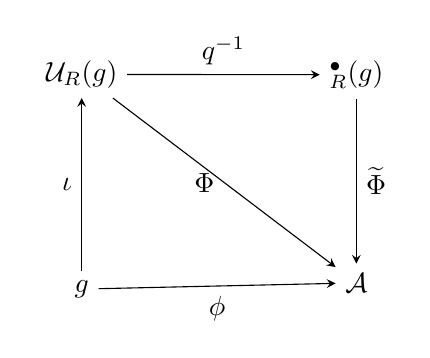
\begin{tikzpicture}
        \matrix (m)[
        matrix of math nodes,
        row sep=6em,
        column sep=7em
        ]
        {
          \mathcal{U}_R(\lie{g})
          & \Sym_R^{\bullet}(\lie{g}) \\
          \lie{g}
          & \mathcal{A} \\
        };
        \draw
        [-stealth]
        (m-1-1) edge node [above] {$\lie{q}^{-1}$}
        (m-1-2) edge node [left] {$\Phi$}
        (m-2-2)
        (m-1-2) edge node [right] {$\widetilde{\Phi}$}
        (m-2-2)
        (m-2-1) edge node [left] {$\iota$}
        (m-1-1)
        (m-2-1) edge node [below] {$\phi$}
        (m-2-2);
    \end{tikzpicture}
\end{center}
from the algebraic theory. The important question is now whether the
algebra homomorphisms $\Phi$ and $\widetilde{\Phi}$ are continuous. This 
question is partly answered by the following result:
\begin{proposition}
    \label{Thm:LCAna:Semi-functoriality}%
    Let $\lie{g}$ be an AE-Lie algebra, $\mathcal{A}$ an associative
    AE-algebra and $\phi \colon \lie{g} \longrightarrow \mathcal{A}$
    is a continuous Lie algebra homomorphism.  If $R \geq 0$, then the
    induced algebra homomorphisms $\Phi$ and $\widetilde{\Phi}$ are
    continuous.
\end{proposition}
\begin{proof}
    We define an extension of $\Phi$ on the whole tensor algebra
    again:
    \begin{equation*}
        \Psi \colon
        \Tensor_R^{\bullet}(\lie{g})
        \longrightarrow
        \mathcal{A},
        \quad
        \Psi
        =
        \widetilde{\Phi} \circ \Symmetrizer
    \end{equation*}
    It is clear that if $\Psi$ is continuous on factorizing tensors,
    we get the continuity of $\widetilde{\Phi}$ and of $\Phi$ via the
    infimum argument. So let $p$ be a continuous semi-norm on
    $\mathcal{A}$ with its asymptotic estimate $q$ and $\xi_1, \ldots,
    \xi_n \in \lie{g}$. Since $\phi$ is continuous, we find a
    continuous semi-norm $r$ on $\lie{g}$ such that for all $\xi \in
    \lie{g}$ we have $q(\phi(\xi)) \leq r(\xi)$. Then we have
    \begin{align*}
        p \left(
        \Psi \left(
        \xi_1 \tensor \cdots \tensor \xi_n
        \right) \right)
        & =
        p \left(
        \widetilde{\Phi} \left(
        \xi_1 \star_{zG} \cdots \star_{zG} \xi_n
        \right) \right)
        \\
        & =
        p( \phi(\xi_1) \cdots \phi(\xi_n) )
        \\
        & \leq
        q( \phi(\xi_1) )
        \cdots
        q( \phi(\xi_n) )
        \\
        & \leq
        r(\xi_1) \cdots r(\xi_n)
        \\
        & \leq
        r_R(\xi_1 \tensor \cdots \tensor \xi_n),
    \end{align*}
    where the last inequality is true for all $R \geq 0$.
\end{proof}


Although this is a nice result, our construction fails to be
universal, since the universal enveloping algebra endowed with our
topology is \emph{not} AE in general. This is even very easy to see:
\begin{example}
    Take $\xi \in \lie{g}$, then we know that $\xi^{\tensor n} =
    \xi^{\ostar_G n} = \xi^n$ for $n \in \mathbb{N}$ where the formal
    parameter is $z = 1$. Let $R > 0$ and $p$ a continuous semi-norm
    in $\lie{g}$ then we find
    \begin{equation}
        p_R(\xi^n)
        =
        n!^R p(\xi)^n
        =
        \frac{n!^R}{c^n} q(\xi)^n
    \end{equation}
    for $c = \frac{p(\xi)}{q(\xi)}$ for a different semi-norm $q$ with
    $q(\xi) \neq 0$.  But since the $\frac{n!^R}{c^n}$ will always
    diverge for $n \rightarrow \infty$ we will never get an asymptotic
    estimate for $p_R$.
\end{example}
Nevertheless, we can draw a nice conclusion from
Proposition~\ref{Thm:LCAna:Semi-functoriality}:
\begin{proposition}
    \label{Thm:LCAna:ContinuousRepresentations}%
    Let $R \geq 1$ and $\mathcal{U}_R(\lie{g})$ the universal
    enveloping algebra of an AE-Lie algebra $\lie{g}$, then for every
    continuous representation $\phi$ of $\lie{g}$ into the bounded
    linear operators $\Bounded(V)$ on a Banach space $V$ the induced
    homomorphism of associative algebras $\Phi \colon
    \mathcal{U}(\lie{g}) \longrightarrow \Bounded(V)$ is continuous.
\end{proposition}
\begin{proof}
    This follows directly from
    Proposition~\ref{Thm:LCAna:Semi-functoriality} and $\Bounded(V)$
    being a Banach algebra.
\end{proof}
\begin{remark}
    \label{Rem:LCAnaBCHConvergence}
    ~
    \begin{remarklist}
    \item \label{item:FiniteDimRepsContinuous} From this, it follows
        in particular that for all finite-dimensional Lie algebras all
        finite-dimensional representations on some vector space $V$
        extend to continuous algebra homomorphisms
        $\mathcal{U}_R(\lie{g}) \longrightarrow
        \operatorname{End}(V)$. For representations on
        infinite-dimensional Banach or Hilbert spaces, the statement
        is typically rather irrelevant, since there one rarely has
        norm-continuous representations, but merely strongly
        continuous ones.
    \item In \cite{pflaum.schottenloher:1998a} Schottenloher and
        Pflaum mention an alternative topology on
        $\mathcal{U}(\lie{g})$ for finite-dimensional Lie algebras:
        They took the coarsest locally convex topology, such that all
        finite-dimensional representations of $\lie{g}$ extend to
        continuous algebra homomorphisms. This topology is in fact
        even locally m-convex. Our topology which uses the grading on
        $\Sym_R^{\bullet}(\lie{g})$ is different from that: As we have
        seen in Proposition~\ref{Thm:LCAna:ContinuousRepresentations},
        it is finer for $R \geq 0$ and even strictly finer for $R >
        0$. For the interesting case $R \geq 1$ it is ''just'' locally
        convex, but its advantage (for our purpose) is that it
        respects the grading, which is helpful for the holomorphic
        dependence on the formal parameter. 
    \end{remarklist}
\end{remark}





% Chapter 6
%


%
% Chapter 6 of my master thesis:
% The nilpotent case
%

\chapter{Nilpotent Lie algebras}

\section{An overview}
\label{sec:chap6_overview}
 - Reference to the counter-example before, no big change
 - Yet: Projective Limit
 - Module structure
 - Generalizations to nilpotency
 
 
 
\section{The Heisenberg and the Weyl algebra}
\label{sec:chap6_HeisenbergWeyl}


 
\section{The projective limit} 
\label{sec:chap6_ProjLim} 
 
 
 
\section{A module structure}
\label{sec:chap6_Modules}
 
\subsection{Generic case and a counter-example}

\subsection{Nilpotent case and good news}



\section{Banach Lie algebras and the finite-dimensional case}
\label{sec:chap6_TheEProperty}

\subsection{Generalizations of nilpotency}

\subsection{A new projective Limit}

\subsection{A result for the finite-dimensional case}




% Chapter 7
%


%
% Chapter 7 of my master thesis:
% The Hopf algebra structure
%

\chapter{The Hopf algebra structure}

\section{The co-product}
\label{sec:chap7_Coproduct}

\subsection{A formula for the co-product}

\subsection{Continuity for the co-product}



\section{The whole Hopf algebra structure}
\label{sec:chap7_HopfAlgebra}




% ============================================================================
% ////////////////////////////////////////////////////////////////////////////





% ============================================================================
% 			Appendix Part
% ============================================================================

\begin{appendices}

  
\chapter{Important theorems in Lie theory}

\section{The Poincar\'e-Birkhoff-Witt theorem}
\label{sec:AppA_PBW}

\section{The Integral form of Baker-Campbell-Hausdorff}
\label{sec:AppA_BCH}

  
  
\chapter{Locally convex algebras}

\section{Locally convex algebras with entire calculus}
\label{sec:AppB_Entire}

\section{Locally m-convex and AE-algebras}
\label{sec:AppB_AEvsLMC}


  
  
\chapter{More explicit formulas for the Gutt star product}

\section{Particular Lie algebras}
\label{sec:AppC_SpecialFormulas}

\section{An Idea for a Mathematica Code}
\label{sec:AppC_Mathematica}


\end{appendices}

% ============================================================================
% ////////////////////////////////////////////////////////////////////////////




% ============================================================================
% 			Bibliography Part
% ============================================================================

% Smaller than other text
%

{
  \footnotesize
  \renewcommand{\arraystretch}{0.5}
%<<<<<<< HEAD
%  \bibliographystyle{../../texmf/bibtex/bib/bst/chairx}
%  \bibliography{../../texmf/bib/dqarticle, ../../texmf/bib/dqbook, ../../texmf/bib/preprints, ../../texmf/bib/dqthesis}
%=======
  \bibliographystyle{../../texmf/bibtex/bib/bst/chairx}
  \bibliography{../../bibfiles/bib/dqbook,../../bibfiles/bib/dqarticle,../../bibfiles/bib/dqthesis,../../bibfiles/bib/preprints,../../bibfiles/bib/misc,../../bibfiles/bib/script,../../bibfiles/bib/dqproceeding,../../bibfiles/bib/dqprocentry}
%>>>>>>> a1f8de4c0a6f9bd5e39d68b2474dc33c3f851a86
}

% ============================================================================
% ////////////////////////////////////////////////////////////////////////////





\end{document}
